\chapter{面向投资组合管理的群组交叉对抗学习方法}

\section{问题的提出}

本章面向对冲基金交易决策流程中的投资组合管理环节，重点讨论多资产配置对象选择与资金权重生成问题。这里的资产选择并不是对单一资产涨跌方向的简单判断，而是指在多资产池中识别相对更具配置价值的标的，并进一步形成满足风险约束的组合权重。因此，本章所讨论的投资组合管理任务不是孤立的收益预测场景，而是多资产、多信号与多约束共同作用下的资金配置问题。围绕该场景，本章以群组交叉对抗（GCA）为核心，构建面向投资组合管理的多智能体对抗学习方法。GCA用于组织异构智能体进行多对多博弈，并在多资产之间比较相对强弱、控制组合风险敞口，将预测信号转化为更稳定的组合权重。需要强调的是，本章的研究边界落在投资组合管理本身，即回答“在多个资产之间如何形成更稳健的配置关系”这一问题；后续章节涉及的因子解释、结构识别、执行优化和策略整合，仅作为全文逻辑链条中的后续环节在本章中作必要衔接。

\subsection{传统投资组合管理方法的局限性}
% ===== 第一段：研究背景与现实意义 =====
金融时间序列预测是量化投资领域的核心挑战之一，其目标是从历史价格、成交量及其他市场数据中挖掘有效信息，以指导资产配置决策。早期金融预测研究主要依赖自回归、移动平均等统计时间序列模型，这类方法为金融时序的均值动态刻画提供了基础工具\cite{box2015time}。但是，对投资组合管理而言，仅说明收益均值的变化还不够，因为组合配置同时受到波动、相关性和风险暴露的共同约束。

在风险建模层面，单纯刻画条件均值并不足以解释金融市场中普遍存在的波动聚集现象。条件异方差框架将条件异方差引入金融序列分析，为收益波动与风险度量提供了重要方法基础\cite{engle2001garch}。这一类研究提醒本文，投资组合管理中的预测结果不能只看方向是否正确，还必须判断该预测所对应的风险暴露是否可被组合层面承受。

广义自回归条件异方差模型进一步扩展了波动率动态刻画能力，成为金融市场风险管理中的经典工具\cite{bollerslev1986generalized}。因此，资产收益预测必须同时面对“收益是否可预测”和“预测结果是否具有风险可承受性”两个问题。对于本章而言，这也意味着模型输出需要进一步转化为满足风险约束的组合权重，而不能停留在单一收益序列的拟合层面。

从组合配置角度看，预测模型的意义并不止于降低数值误差，而在于为资产配置提供可执行的风险收益判断。现代投资组合理论强调在收益与风险之间进行权衡，奠定了均值—方差框架的基础\cite{markowitz1952portfolio}。这一理论基础说明，组合管理的核心并不是挑出某一个预测收益最高的资产，而是在多个资产之间权衡收益、风险和相关性。

在此之后，资本资产定价模型从系统性风险定价角度解释了资产收益与风险暴露之间的关系\cite{sharpe1964capital}。这使得投资组合问题进一步从“预测收益”转向“识别收益背后的风险来源”。对于对冲基金交易而言，如果模型只输出单资产预测值，而不能区分该收益来自可承担的风险补偿还是不可控的系统性暴露，预测结果仍然难以直接用于配置。
进一步地，Black--Litterman 模型将市场均衡收益与投资者观点结合，为多资产配置中的先验约束与风险控制提供了常用框架\cite{black1992global}。由此可见，第二章并不是单纯追求价格序列预测精度，而是需要把预测信号放入组合权重、风险敞口和资金配置稳定性之中加以考察。

这些经典理论共同说明，面向对冲基金的预测模型不能只围绕单个价格序列展开，还需要服务于组合权重分配、风险敞口控制与长期收益稳定性。在真实交易环境中，预测结果只有经过资产比较、仓位控制与组合风险约束，才能最终转化为投资绩效。因此，本章讨论的核心问题是投资组合管理中的资产配置：模型不仅要预测单个资产的局部走势，还要比较不同资产之间的相对价值，并形成可执行的多资产权重分配方案。

随着机器学习方法的发展，支持向量机等非线性模型被用于金融时间序列预测，显示出相较传统线性模型的表达优势\cite{tay2001application}。这类模型的重要意义在于突破线性假设，为捕捉价格与成交量等变量之间的非线性关系提供了可能。但从投资组合管理角度看，非线性预测本身仍然只是配置决策的输入环节。

随后，长短期记忆网络通过门控记忆扩展金融时序建模能力\cite{hochreiter1997long}。这表明模型开始从静态特征拟合转向序列依赖建模，但其输出若不能被进一步比较和约束，仍可能停留在单资产预测层面。
门控循环单元在保持序列表达能力的同时简化结构\cite{cho2014learning}。这种结构简化有助于提升训练效率，但也提示本文需要在模型复杂度、收益预测稳定性和组合可执行性之间保持平衡。

自注意力序列模型则进一步强化长程依赖刻画\cite{vaswani2017attention}。这些模型分别代表了从非线性分类、循环记忆到全局依赖建模的技术演进，为处理金融序列中的复杂依赖关系提供了基础。与此同时，本章关注的重点并不是单纯选择更强的序列模型，而是如何把不同模型的预测结果组织成可交叉校验的多资产配置依据。

在金融应用中，长短期记忆网络已被用于股票市场方向预测，并在部分样本外区间表现出优于传统模型的效果\cite{fischer2018deep}。这说明深度序列模型能够提升方向预测能力，但方向预测并不等同于投资组合管理。组合管理还需要回答哪些资产更值得配置、配置多少以及在何种风险条件下配置。
针对长序列预测问题，Informer通过稀疏注意力机制提高建模效率\cite{zhou2021informer}。长序列建模能力的提升有助于扩展历史信息窗口，但在金融市场中，较长的信息窗口也可能引入过时状态和噪声，因此仍需要与市场状态筛选和组合约束结合。

Autoformer则利用分解结构与自相关机制强化长期依赖刻画\cite{wu2021autoformer}。这些研究扩展了模型处理时间依赖的能力，但组合管理关心的并不只是时序拟合本身。若模型只能改善单资产预测误差，而不能稳定比较多资产相对收益并生成可约束的组合权重，其优势仍难以转化为组合层面的风险收益表现。

在资产配置层面，投资组合自注意力序列模型等方法直接面向组合权重与风险调整收益进行建模，说明注意力机制已开始从预测环节延伸到投资组合决策环节\cite{kisiel2022portfolio}。这一变化表明，金融模型的目标不应局限于提高预测精度，还需要使输出能够对应资金配置和风险调整收益。
与此同时，深度强化学习投资组合管理研究表明，端到端地学习资产权重配置具有一定可行性\cite{jiang2017deep}。这类方法把投资组合作为序贯决策问题处理，使模型输出能够直接对应资产权重或交易动作。但在本章语境中，端到端并不意味着可以忽略模型之间的交叉校验，因为多资产配置中的错误预测会通过权重放大并转化为组合风险。

从本章的问题看，上述研究提供的启示并不是“用更复杂的模型替代传统模型”这么简单，而是说明投资组合管理需要把收益预测、权重生成和风险约束同时纳入建模过程。在鲁棒性方面，对抗深度强化学习投资组合方法表明，对抗训练可以服务于组合管理中的稳健决策\cite{liang2018adversarial}。这提示本文，投资组合管理中的对抗机制应当面向市场扰动和模型偏差，而不是仅作为生成模型形式上的装饰。

强化学习也被用于引入增强的资产运动状态，以改善投资组合管理中的状态表达与动作选择\cite{ye2020reinforcement}。因此，本章进一步关注如何通过多智能体之间的交叉评估，将单一模型输出转化为更稳健的多资产配置依据。
然而，将上述技术直接应用于金融预测时，仍会面临一系列独特挑战。首先，金融数据具有极低的信噪比，历史价格中的有效信息含量有限，大量波动来自随机交易行为与外生冲击\cite{lo2017economics}。这意味着即使模型在训练样本中捕捉到局部规律，也不能直接判断该规律具有稳定的交易价值。
同时，股票收益的随机游走假说长期受到实证检验，收益可预测性本身具有样本依赖与周期依赖特征\cite{lo1988stock}。因此，本章更强调多模型之间的交叉评估和组合层面的风险约束，避免将短期样本中的偶然预测优势直接放大为资产配置决策。
其次，金融市场具有显著的非平稳性，宏观冲击、流动性变化与参与者行为变化都可能导致训练样本与未来样本之间出现分布差异。以 2020 年新冠疫情期间的跨市场冲击为例，市场避险关系和资产间联动结构均可能出现阶段性变化\cite{conlon2020time}。因此，传统的均方误差损失难以有效反映投资组合的风险调整后收益特性，也难以保证模型在分布漂移环境下保持稳定。

\subsection{金融场景下多智能体博弈建模的挑战}
投资组合交易之所以需要多智能体建模，是因为其研究对象并不是单一资产的价格方向，而是多个资产之间相对收益、风险暴露、资金权重和市场状态共同作用下的动态配置过程。不同资产之间存在相关性变化、流动性差异和风险传导关系，单一模型即使能够在局部样本上取得较低预测误差，也未必能够稳定处理截面比较、仓位分配和组合层面的回撤控制。多智能体建模的意义在于，将不同资产视角、不同模型归纳偏置和不同风险约束组织为可交互的学习主体，使系统能够通过竞争、校验和协同约束刻画多资产配置中的动态博弈关系。

在这一背景下，多资产信号的不稳定性、不同品种之间的权重偏差以及风险暴露的阶段性变化，构成本章多智能体建模首先需要面对的问题。若模型仅对单一资产或单一生成器进行优化，则容易在市场状态切换时放大局部预测误差，进而影响组合层面的资金分配和回撤控制。因此，本节从多资产配置需求出发，讨论生成器、判别器与异构模型群之间如何形成可交叉评估、可动态校验的博弈结构。

生成对抗网络通过生成器与判别器之间的对抗博弈学习数据分布，已在图像生成、自然语言处理等领域得到广泛应用\cite{goodfellow2014generative}。对于本章而言，生成对抗思想的价值不在于生成一个孤立的价格序列，而在于利用判别器反馈约束预测序列的分布特征，使模型输出更接近可用于配置决策的市场状态描述。

标准生成对抗网络在训练中容易出现不稳定、模式崩溃和收敛困难等问题\cite{gui2023review}。这一问题对金融任务尤其敏感，因为金融收益分布本身具有强噪声、厚尾和状态切换特征，训练不稳定会直接影响后续组合权重的可靠性。

围绕训练不稳定问题，Arjovsky等人提出瓦瑟斯坦生成对抗网络，用推土机距离替代Jensen--Shannon 散度以缓解梯度消失问题\cite{arjovsky2017wasserstein}。这一类改进主要改变对抗训练的距离度量，为稳定学习分布差异提供了基础，但它仍然没有回答多资产配置中不同生成器如何分工的问题。

在此基础上，判别器约束和训练正则化进一步从梯度反馈层面改善对抗学习的稳定性。Gulrajani等人引入梯度惩罚以满足Lipschitz约束\cite{gulrajani2017improved}。这一方法说明，判别器约束的平滑性会直接影响生成器获得的梯度信号；在本文语境中，这对应于预测输出能否获得稳定的分布校正反馈。Miyato等人进一步通过谱归一化约束判别器权重矩阵的谱范数\cite{miyato2018spectral}。这类结构层面的稳定化处理提示本文，多判别器结构不能只增加判别器数量，还必须保证不同判别器输出的反馈信号不会放大金融噪声。Brock等人在大规模生成对抗网络中引入正交正则化与大规模训练策略\cite{Brock:2018rok}。上述研究共同说明，对抗训练的稳定性不仅取决于生成器能力，也取决于判别器反馈、正则约束和训练过程之间的协同关系。对于投资组合管理任务而言，本文更关注的是如何把这种稳定反馈转化为多资产预测结果之间的相互校验，而不是单纯提高样本生成质量。

针对时序数据，Yoon等人提出的时间序列生成对抗网络将对抗训练与逐步监督信号结合，为序列生成建模提供了代表性框架\cite{10.5555/3454287.3454781}。但是，金融数据的强非平稳性和极端事件仍会削弱这类模型的稳定性。本文借鉴时序对抗建模的思想，并不是为了生成完整的“假市场序列”，而是为了约束给定输入条件下预测输出与真实市场状态之间的联合关系。

单一生成器-判别器结构在分布漂移条件下容易性能衰退，多生成器架构虽然能够扩大覆盖范围，但在极端行情下也可能同步退化并形成局部共识幻觉\cite{ghosh2017multi}。因此，在投资组合管理中，仅提高生成质量并不足够，还需要引入多模型交叉评估、异构信号约束与组合权重输出机制。将生成对抗网络用于投资组合管理的原因在于，判别器可以作为“统计检验器”，约束生成器输出的多资产预测序列在分布特性上接近真实市场数据，并使这些预测信号进一步服务于组合权重分配。

从时间序列生成角度看，循环条件生成对抗网络在真实值时间序列生成任务中的应用说明，对抗式生成模型能够在一定程度上保留时间依赖结构\cite{esteban2017real}。这类研究的启示在于，金融时序预测不应只关注单点误差，还需要关注预测序列是否保留了市场变化过程中的条件依赖关系。
时间序列生成对抗网络进一步将对抗损失与逐步监督信号结合，为时间序列生成建模提供了代表性框架\cite{yoon2019time}。这些研究说明，对抗约束可以补充传统均方误差损失的不足；但在本章的组合管理任务中，分布约束最终仍需要回到多资产相对收益、权重生成和风险调整收益这三个配置目标上。

然而，标准 生成对抗网络 框架采用“一对一”（one-to-one）的生成器-判别器配对架构，在金融预测场景中面临四重主要挑战。
第一，模式崩塌（Mode Collapse）问题在金融时间序列中尤为突出。金融市场的收益率分布通常呈现尖峰厚尾、偏态等复杂特性，且在不同市场机制下表现出显著差异，早期关于投机价格变动的研究已经揭示了这类厚尾与非常态波动特征\cite{mandelbrot1963variation}。单一生成器在对抗训练中容易陷入“安全模式”，仅学习数据分布的少数主导模式，而忽视尾部风险和极端行情。
这一问题在多资产投资组合预测中更为严重：生成器可能只学会预测少数高流动性品种，而对低流动性品种产生系统性偏差。多智能体多生成器 生成对抗网络 的研究表明，通过多个生成器之间的竞争可以提升数据模式覆盖能力\cite{ghosh2017multi}。这提示仅依赖单生成器结构难以满足多资产配置对信号覆盖、权重分散和风险约束的要求，需要通过多模型交叉评估提高复杂金融数据分布的覆盖能力。

第二，“一对一”博弈拓扑限制了模型的多样性表达。理论上，多个具有不同归纳偏置的生成器可以分别专注于学习数据分布的不同方面，例如 门控循环单元更适合短期均值回归特征，自注意力序列模型更适合长期结构依赖。但在标准 生成对抗网络 框架下，不同生成器之间缺乏有效的竞争与协作机制，容易趋同于相似的预测输出。
围绕对抗训练稳定性，瓦瑟斯坦生成对抗网络从距离度量角度缓解了标准生成对抗网络训练不稳定问题，但其重点仍在单生成器分布逼近\cite{arjovsky2017wasserstein}。这类方法解决的是“如何让单个对抗系统更稳定”的问题，而不是“如何让多个预测模型在组合管理中形成互补分工”的问题。
谱归一化则通过约束判别器 Lipschitz 常数提高对抗训练稳定性，为复杂对抗系统提供了基础稳定化手段\cite{miyato2018spectral}。这些方法能够改善训练过程，但并未直接解决多个生成器之间如何分工的问题。
围绕多模型协同，相关研究已经从生成器组合、判别器协同和分布区域分工等角度对传统对抗结构进行了扩展。混合生成对抗网络通过多个生成器的概率组合来扩大生成分布的覆盖范围，为多生成器协同提供了参考\cite{hoang2018mgan}。对本文而言，这一思路的启示并不在于简单增加生成器数量，而在于说明不同生成器可以承担不同市场状态或资产关系下的预测职责，从而避免所有模型收敛到同一种输出模式。进一步看，生成器之间的差异只有在判别反馈能够形成多视角约束时，才可能真正转化为组合管理中的交叉校验能力。生成式多对抗网络讨论了多个判别器参与训练时的稳定性问题\cite{durugkar2017generative}。这一方向提示，判别器不应只作为单一真假判断器，而可以分别从不同角度检查生成器输出是否具有合理性。专业化判别器方法则表明，多判别器结构能够让不同判别器分别关注真实分布的不同子区域\cite{choi2022mclgan}。因此，多模型对抗结构的价值并不只是提升模式覆盖范围，更在于为本文后续构建“多生成器—多判别器”的交叉校验关系提供方法依据；但在投资组合管理任务中，模型输出最终还要服务于动态权重配置，因此仍需进一步结合金融市场的非平稳特征进行约束设计。

第三，静态优化范式与金融市场非平稳性之间存在矛盾。传统生成对抗网络在训练完成后，生成器和判别器的参数通常固定不变，而金融市场却具有显著的状态依赖性。大规模市场波动研究表明，市场波动在不同时间阶段会呈现聚集与结构变化特征\cite{plerou2002quantifying}。这意味着，投资组合管理模型面对的并不是稳定不变的数据分布，而是会随市场冲击、流动性变化和资产联动关系调整而持续变化的动态环境。对于多资产组合而言，分布漂移不仅会改变单个资产的收益预测误差，还会改变资产之间的相关性、波动暴露和权重约束条件。自适应市场假说进一步指出，市场有效性与投资者行为会随环境变化而动态演化\cite{lo2004adaptive}。从本文研究对象看，这一观点说明模型不能只在历史样本上获得一次性最优解，还需要在后续市场状态变化中持续校验预测信号和组合权重是否仍然有效。马尔可夫转换模型也从状态切换角度刻画了非平稳经济时间序列，为理解金融市场体制转换提供了经典工具\cite{hamilton1989regime}。这些研究共同说明，固定权重模型在分布漂移场景下可能迅速失效，本章提出的多智能体群组交叉对抗结构需要具备动态校验与更新能力，使系统能够在非平稳环境中维持较稳定的组合权重输出。

第四，训练效率与知识传承存在不足。生成对抗网络的训练过程以极小—极大博弈为本质，梯度信号在判别器与生成器之间来回振荡，容易导致收敛缓慢且不稳定。相关研究从理论角度分析了生成对抗网络训练不稳定的来源与改进方向\cite{arjovsky2017towards}。这一问题在多生成器、多判别器结构中会被进一步放大，因为每个生成器都需要接受判别反馈，多个模型之间还需要维持差异性与协同性。两时间尺度更新规则为生成对抗网络稳定训练提供了另一类实证与理论依据\cite{heusel2017gans}。然而，这类稳定化策略主要面向训练过程本身；在投资组合管理场景下，系统还必须考虑新数据到达、模型性能衰退以及旧模型知识如何被新模型继承的问题。知识蒸馏通过教师模型向学生模型传递软标签信息，为模型压缩与知识迁移提供了经典范式\cite{hinton2015distilling}。这一思路说明，模型更新不一定只能依赖从头训练，也可以通过已有模型向新模型传递有效知识来降低重复训练成本。深度互学习进一步表明，多个模型可以在相互学习过程中共同提升，而不必固定单一教师模型\cite{zhang2018dml}。由此可见，投资组合管理需要超越传统单模型和一对一对抗结构，在生成器、判别器与异构模型群之间建立可交叉评估、可动态协同、可传承知识的建模关系。与后续章节分别讨论高维金融因子建模、时序结构识别、交易执行优化和策略整合不同，本章首先解决的是多智能体如何服务于资产配置对象选择和资金配置的问题。

基于上述分析，本章需要解决的关键问题可以凝练为：在多资产组合管理中，如何在低信噪比、非平稳和多资产联动关系不断变化的条件下，稳定识别不同资产之间的相对配置价值，并将预测信号转化为风险约束下的组合权重。针对这一问题，GCA并不是简单增加模型数量，而是通过多生成器、多判别器之间的群组交叉对抗，使不同智能体在异构视角下相互校验，从而缓解单一模型导致的信号趋同、权重偏差和风险暴露失衡。由此，2.1提出的问题将在2.3的问题建模中被形式化，并在2.4的GCA算法设计中得到对应回应。

\section{相关工作}

本节围绕投资组合管理任务所依赖的相关研究展开梳理，重点说明现有方法如何从静态组合优化、深度学习资产配置逐步走向多模型协同与对抗式学习。与单纯讨论生成模型不同，本节关注的是这些研究如何服务于资产配置对象选择和资金配置的组合管理问题。

首先，传统投资组合管理研究以收益—风险权衡为核心，强调在多个资产之间进行权重分配和风险暴露控制。随着市场状态不断变化，静态权重配置方法难以充分刻画多资产之间的动态相关关系，因此后续研究逐渐引入机器学习与深度学习方法，以提高资产收益预测、风险估计和仓位调整的自适应能力。深度强化学习投资组合管理进一步将资产配置表示为序贯决策问题，使模型能够直接输出资产权重或交易动作。与2.1中对方法背景的介绍不同，本节更关注这些研究在投资组合管理任务中的具体不足，即它们是否能够把多资产相对关系、模型间校验和组合权重输出组织为同一个闭环。

其次，多智能体学习为投资组合管理中的多模型协同提供了方法基础。从多智能体学习角度看，多智能体 actor-critic 方法说明，不同智能体之间的交互关系可以被显式纳入学习过程\cite{lowe2017multi}。在多资产配置场景中，不同智能体可以对应不同时间尺度、不同模型结构或不同资产视角，通过协同与竞争共同形成组合决策。与单一模型相比，多智能体结构有助于降低某一模型对特定市场状态的过度依赖。

此外，对抗式学习为投资组合管理中的稳健性提供了重要启发。从鲁棒学习角度看，鲁棒对抗强化学习表明，在训练阶段引入对手或扰动有助于提升策略在不确定环境中的稳健性\cite{pinto2017robust}。这一思想与金融市场中的多主体竞争、策略交互和环境非平稳特征具有一致性。对于投资组合管理而言，对抗式训练的意义不只是生成更逼真的时间序列，而是通过判别反馈约束预测分布，使模型输出更适合后续资产权重配置。

最后，生成对抗学习和多模型协同研究为金融序列的分布约束与模型集成提供了重要工具。但在投资组合管理任务中，关键问题并不只是生成更逼真的时间序列，而是如何让多个异构模型在统一评价尺度下相互校验，并将其输出稳定转化为组合权重。因此，相关工作的不足主要体现在“多资产信号—模型交叉评估—组合配置输出”之间尚未形成闭环。

上述研究表明，投资组合管理已经从静态组合优化扩展到深度学习和强化学习驱动的动态资产配置；但在多资产信号稳定性、单模型配置偏差和模型间交叉校验方面仍存在不足。对于对冲基金交易而言，这些不足最终会影响资产配置对象识别与资金权重分配的稳定性：若模型只能给出单资产预测结果，而缺乏对多资产相对关系、组合权重和风险暴露的联合约束，预测优势就难以稳定转化为组合收益。基于此，本章提出面向投资组合管理的群组交叉对抗学习方法，将多个异构生成器和判别器组织为交叉博弈结构，以约束多资产配置过程中的信号稳定性、权重生成和组合风险。


\section{任务描述}

本节在相关工作基础上进一步明确本章的任务对象，并将2.1中提出的多资产配置问题转化为可建模的优化任务。投资组合管理并不等同于单资产方向预测，而是需要将多资产收益预测结果转化为组合权重，并在资金中性、风险调整收益与分布一致性等约束下形成可执行的配置决策。由此，本节先定义投资组合预测问题，再说明多资产收益预测与权重生成方式，最后给出本章方法需要满足的优化目标。这样处理的目的，是把资产配置任务具体落实为多资产相对收益比较、组合权重生成和风险调整收益优化三个环节，为后续GCA方法设计提供明确的任务边界。

\subsection{投资组合预测问题建模}

给定历史市场数据序列 $X = \{x_1, x_2, \ldots, x_T\}$，其中每个时刻的特征向量 $x_t$ 包含该资产的开盘价、最高价、最低价、收盘价与成交量及相关技术指标（如 指数平滑异同移动平均线、相对强弱指数、随机指标、真实波幅、布林带等）。模型的目标是基于历史窗口 $W$ 预测未来 $H$ 步的收益率序列：
\[
\hat{r}_{t+1:t+H} = f(x_{t-W+1:t}; \theta)
\]
其中 $\theta$ 为模型参数，$f(\cdot)$ 为预测函数。

需要说明的是，本章中的预测目标并不是单一时点的类别标签，而是给定历史市场窗口后的未来收益序列。为便于后续方法表述，本文将历史窗口 $x_{t-W+1:t}$ 视为条件输入，将真实未来收益序列记为 $r_{t+1:t+H}$，将模型输出记为 $\hat{r}_{t+1:t+H}$。因此，后文若使用 $y$ 表示监督目标，其含义对应真实未来收益序列，而非判别器训练中的二分类标签；判别器所使用的标签 $1/0$ 仅用于区分真实条件样本对与模型预测样本对。通过这一约定，可以避免将收益预测目标与对抗训练标签混同。


\subsection{多资产收益预测与组合权重生成}

在多资产投资组合场景下，设投资组合包含 $K$ 个资产，模型需同时预测 $K$ 个资产的未来收益率向量 $\hat{r}_t \in \mathbb{R}^K$。进一步，通过策略函数 $\phi(\cdot)$ 将预测收益率转化为资产权重 $w_t \in \mathbb{R}^K$，满足资金中性约束 $\sum_{i=1}^K w_{t,i} = 0$。具体采用连续多空策略：
\[
w_{t,i} = \frac{\hat{r}_{t,i} - \bar{r}_t}{\sum_{j=1}^K |\hat{r}_{t,j} - \bar{r}_t|}
\]
其中 $\bar{r}_t = \frac{1}{K}\sum_{j=1}^K \hat{r}_{t,j}$ 为截面均值。该策略专注于捕捉资产间的相对强弱关系（阿尔法），而非市场的系统性风险（贝塔）。


\subsection{组合风险约束与优化目标}

优化目标为最大化风险调整后收益，同时满足预测保真度和分布一致性约束：
\[
\max_{\theta} \mathcal{L}_{SR}(\theta) - \lambda_1 \mathcal{L}_{均方误差}(\theta) - \lambda_2 \mathcal{L}_{生成对抗网络}(\theta)
\]
其中 $\mathcal{L}_{SR}$ 为夏普比率损失（风险调整收益），$\mathcal{L}_{MSE}$ 为均方误差损失（数值保真度），$\mathcal{L}_{GAN}$ 为对抗损失（分布一致性）。从任务含义看，均方误差项用于保证资产收益预测的基本可用性，对抗损失用于约束预测序列与真实市场分布的一致性，夏普比率目标则将模型输出与投资组合的风险调整收益直接连接。三者共同对应本章问题中的信号稳定性、权重生成合理性和风险约束要求。



\section{群组交叉对抗方法}

本节围绕GCA展开方法设计。前一节已经给出投资组合预测、权重生成与优化目标，本节重点说明GCA如何通过异构生成器、判别器与组间交叉评估机制服务于多资产配置任务。具体而言，异构生成器用于从不同时间尺度和模型归纳偏置中提取多资产收益信号，多判别器用于从分布一致性角度检验生成结果，组间交叉对抗则用于避免单一模型在特定资产或特定市场状态上形成过度依赖。由此，GCA对2.1提出的三个问题形成直接回应：以多模型交叉评估提升信号稳定性，以多生成器竞争降低权重偏差，以风险调整目标约束组合输出。其他知识传递或状态修复机制只作为后续章节展开的辅助接口，不作为本章的主体方法。

需要说明的是，本文中的“生成器”并非传统生成对抗网络中从随机噪声直接生成样本的网络，而是在给定历史市场窗口和多资产状态特征条件下，输出未来收益预测或组合配置依据的条件预测模型。将其称为生成器，是因为该模型输出并不只接受点对点预测误差约束，还需要进入判别器构成的对抗训练过程，在数值保真度、条件分布一致性和组合风险调整目标之间同时接受约束。换言之，本章关注的并不是生成逼真的无条件金融样本，而是生成能够服务于投资组合权重配置的稳健预测输出。

%本节回顾与本章研究密切相关的三个领域的研究进展：多生成器生成对抗网络、知识蒸馏与模型压缩以及金融时间序列预测中的深度学习方法。通过对现有文献的系统梳理，明确当前研究的主要进展与不足，为本章的研究动机提供理论依据。

%\subsection{多生成器生成对抗网络}

% \subsubsection{问题域与方法发展}

%生成对抗网络（Generative Adversarial Network, GAN）自Goodfellow等人 \cite{goodfellow2014generative}提出以来，已成为生成建模领域的重要框架之一。GAN通过构建生成器与判别器之间的min-max对抗博弈，使生成器学习逼近真实数据分布。然而，标准GAN的训练过程存在显著的不稳定性问题，模式崩塌（mode collapse）是其中最为突出的核心问题，即生成器只学习到数据分布中的少数模式，而无法完整覆盖真实分布的多样性 \cite{arjovsky2017wasserstein}、\cite{mescheder2018training}。

%针对模式崩塌问题，相关研究者从不同角度提出一系列改进策略。Wasserstein GAN（WGAN） \cite{arjovsky2017wasserstein} 通过引入Wasserstein距离替代Jensen--Shannon 散度，实现了更稳定的训练过程。谱归一化 \cite{miyato2018spectral} 通过对判别器的权重矩阵进行谱归一化，约束判别器的Lipschitz常数，进一步提升训练稳定性。然而，这些方法主要关注单生成器场景下的训练稳定性，未能从根本上解决生成器多样性不足的问题。

% \subsubsection{多生成器架构的进展}

%多生成器架构作为缓解模式崩塌的另一重要研究方向，逐渐受到研究者的广泛关注。Ghosh等人 \cite{ghosh2017multi} 提出的MAD-GAN（Multi-Agent Diverse GAN）通过多个生成器共享一个判别器，要求判别器识别每个样本由哪个生成器产生，迫使其通过竞争学习不同的数据模式。Hoang等人 \cite{hoang2018mgan} 提出的MGAN（Mixture GAN）采用概率混合的方式组合多个生成器的输出，理论分析证明在均衡状态下，生成器混合分布与真实数据分布之间的Jensen-Shannon散度最小化，同时生成器之间的散度最大化，从而直接解决模式崩塌问题。Durugkar等人 \cite{durugkar2017generative} 进一步提出了多生成器多判别器架构（MGMD），通过引入多个判别器从不同角度评估生成样本。

%而MCL-GAN \cite{choi2022mclgan} 所提出的专业化判别器是多判别器架构的重要突破。该方法受多选择学习（Multiple Choice Learning）启发，让每个判别器专注于区分真实数据的一个子集，同时允许生成器自动找到潜在空间与真实数据空间之间的对应关系。这种设计在一定程度上缓解了模式崩溃问题，并通过共享骨干网络将计算成本控制在可接受范围内。然而，该方法的协作机制仅限于特征共享层面，未能建立生成器与判别器之间的深层对抗-协作关系。

% \subsubsection{金融应用与现有不足}

%在金融时间序列领域，研究者也将多生成器架构引入到序列生成任务中。Yoon等人 \cite{yoon2019time} 提出的TimeGAN在保留对抗损失的基础上引入了逐步监督损失（stepwise supervised loss），使模型更好地学习时序条件分布，该工作发表于NeurIPS 2019。Zhou等人 \cite{zhou2020mdgan} 提出的MDGAN采用多判别器结构增强对时序模式的评估能力。FinGAN \cite{wiese2020leveraging} 将多生成器架构应用于金融波动率建模，在衍生品定价任务上取得了显著提升。

%尽管现有多生成器GAN相关研究已取得了显著进展，但在以下方面仍存在明显不足：第一，不同生成器之间缺乏深度的竞争-协作机制，容易出现"伪多样性"——即生成器虽然架构不同，但预测输出高度相关，未能真正实现模式覆盖的扩展；第二，现有方法主要关注静态的模型集合，缺乏对数据分布时变性的自适应能力；第三，缺乏对生成器健康状态的监控机制，无法在模型性能衰退时自动触发修复。

%\subsection{知识蒸馏与模型压缩}

% \subsubsection{知识蒸馏的基本理论与单向模式}

%知识蒸馏（Knowledge Distillation）最初由Hinton等人 \cite{hinton2015distilling} 提出，旨在将大型教师模型（teacher model）的知识迁移到轻量级学生模型（student model），实现模型压缩的同时保持预测性能。其核心思想是让学生模型学习教师模型的"软标签"（soft labels），而非仅学习硬标签（hard labels），从而传递教师模型在类别关系上的暗含知识。

%传统知识蒸馏采用单向的知识传递模式，即教师模型参数固定，学生模型从教师输出中学习。这种模式在模型压缩场景中效果显著，但存在如下局限：其一，当学生模型能力接近教师模型时，蒸馏信号趋于消失，训练效率降低；其二，单向传递无法利用学生模型学习过程中的有价值信息，造成知识浪费；其三，教师模型本身的偏差会完整传递到学生模型，无法纠正。

% \subsubsection{双向知识流动与动态模型选择}

%为克服单向蒸馏的局限，研究者提出了多种双向知识流动机制。Zhang等人 \cite{zhang2018dml} 提出的深度互学习（Deep Mutual Learning, DML）让多个学生模型相互学习，每个模型既是教师也是学生，实现了知识的双向传递。Yuan等人 \cite{yuan2020revisiting} 提出的基于标签自蒸馏（Label Self-Distillation）方法，让模型从自身的历史输出中学习，实现知识的跨时态传递。Lee等人 \cite{lee2019self} 进一步提出了跨模型自蒸馏框架，通过模型自身的不同训练阶段实现知识精炼。

%在模型选择与动态组合领域，AutoML和神经架构搜索（Neural Architecture Search, NAS）技术 \cite{elsken2019neural} 提供了自动化模型选择的可能性。然而，这些方法通常需要大量的计算资源，且搜索空间的设计高度依赖人工经验，在金融时序预测场景下的系统性应用仍处于早期阶段。

% \subsubsection{蒸馏机制与对抗学习的结合空白}

%知识蒸馏与模型选择的研究进展为本章的逆向师生蒸馏（S2T）提供了理论基础。然而，现有方法未能将蒸馏机制与对抗学习有机结合，也缺乏在金融时序预测场景下的系统性验证。

%\subsection{面向金融时序预测的深度学习方法}

% \subsubsection{问题背景与传统方法的局限}

%金融时间序列预测是量化投资领域的核心问题。传统计量经济学方法，如自回归移动平均模型（AutoRegressive Moving Average, ARMA）和广义自回归条件异方差模型（Generalized AutoRegressive Conditional Heteroskedasticity, GARCH） \cite{bollerslev1986generalized}、\cite{engle2001arch}，在建模金融数据的条件均值和方差动态方面取得了重要进展。然而，这些线性模型难以捕捉数据中的非线性依赖关系和复杂交互模式。

% \subsubsection{深度学习方法的应用与挑战}

%深度学习技术的引入为金融时间序列建模带来了新的可能性。循环神经网络（Recurrent Neural Network, RNN）及其变体长短期记忆网络（Long Short-Term Memory, LSTM）和门控循环单元（Gated Recurrent Unit, GRU） \cite{hochreiter1997lstm}、\cite{cho2014learning} 能够有效捕捉时间序列中的长程依赖关系，在股价预测 \cite{fischer2018deep}、波动率建模 \cite{li2018deep} 等任务上展现出优于传统方法的性能。Transformer架构 \cite{vaswani2017attention} 通过自注意力机制建模任意位置之间的依赖关系，在自然语言处理取得巨大成功后，也被广泛应用于时间序列分析 \cite{zhou2021informer}、\cite{wu2020autoformer}。

%然而，将深度学习直接应用于金融预测面临独特的挑战。首先，金融数据具有极低的信噪比，历史价格中的有效信息含量极低，大部分为随机噪声 \cite{lo2017economics}。单纯的监督学习容易导致模型过度拟合历史噪声，在样本外表现急剧下降。其次，金融市场具有显著的非平稳性，如2020年新冠疫情、2022年全球通胀等事件易导致数据分布发生剧烈变化 \cite{conlon2020time}。基于历史数据训练的模型在这种"分布漂移"场景下性能衰退严重。第三，金融决策需要同时考虑收益与风险，传统的均方误差（Mean Squared Error, MSE）损失无法反映投资组合的风险调整后收益特性。

% \subsubsection{多角度的改进方案与多模型协同}

%为解决上述问题，研究者从多个角度进行了探索。在损失函数设计上，Kelly等人 \cite{kelly2019deep} 提出了面向金融决策的定制化损失函数，将夏普比率等风险指标纳入优化目标。Fang等人 \cite{fang2020deep} 进一步提出了面向多资产组合优化的对抗训练框架，通过判别器约束生成预测的统计特性。在模型集成方面，种种研究表明，多模型的动态组合能够有效提升预测的鲁棒性 \cite{caruana1997multitask}、\cite{dietterich2000ensemble}。然而，如何设计有效的多模型协同机制仍是开放性问题。

% \subsubsection{GAN在金融预测中的应用与不足}

%将GAN应用于金融预测是近年来的新兴研究方向。

%而生成对抗网络（GAN）凭借其独特的对抗学习特性，为该问题的解决提供了新的技术路径，也成为近年来金融预测领域的新兴研究方向。Esteban等人 \cite{esteban2017real} 提出的Real-valued GAN（RGAN）能够生成逼真的金融时间序列样本。SeqGAN \cite{yu2017seqgan} 将GAN扩展到离散序列生成任务，为金融信号生成提供了新思路。COTED提出了面向金融预测的条件时序对抗网络，在资产收益率预测任务上取得了显著进展。然而，这些方法主要关注单生成器-单判别器架构，未能充分利用多模型协同的潜力。

% \subsection{现有文献的空白与本章贡献}

%综合上述文献的梳理与分析可以发现，当前研究在以下三个方面仍存在系统性空白，这些空白也正是本章的核心研究动机：
%\begin{enumerate}
%\item \textbf{多生成器协同机制的设计不足}：现有方法虽然引入了多个生成器，但缺乏深度的竞争-协作机制来确保生成器之间的多样性。“伪多样性”问题导致集成收益被显著削弱。
%\item \textbf{单向知识传递的效率瓶颈}：传统蒸馏和互学习方法未能与对抗学习有机结合，知识传递的效率和效果受到限制。
%\item \textbf{缺乏模型健康监控与自体再生机制}：现有方法缺乏对模型自身状态的实时监控能力，无法在检测到性能衰退时自动触发修复。
%\end{enumerate}

%针对上述空白，本章提出多智能体群组交叉对抗学习框架（MGCA）。该框架通过三个创新点的系统性协同解决上述问题：群组交叉对抗（GCA）增加模型多样性、逆向师生蒸馏（Student-to-Teacher Distillation, S2T）实现双向知识流动、孪生对抗自体再生（Twin）提供异常监控与自体再生能力。
%现有研究尚缺乏一个系统性的框架来同时应对多样性、知识传递和监控这三个方面的挑战。单独的改进（如改进损失函数、引入多生成器或应用蒸馏机制）往往只能部分缓解问题，难以全面应对金融时间序列预测中多模型协同学习的复杂性。因此，设计一个有机整合多个创新点的完整框架，使其在金融预测任务中充分发挥协同效应，成为了一个迫切的研究需求。
\subsection{群组交叉对抗的建模动因与基本假设}

群组交叉对抗机制是多生成器-多判别器结构的核心组成部分，也是本章面向投资组合管理任务的主要方法。其设计目的不是简单增加模型数量，而是通过异构生成器与判别器之间的交叉对抗学习，建立一个能够服务多资产收益判断、组合权重生成和风险暴露约束的群组博弈结构，从而降低单一模型在复杂资产池中出现信号趋同、模式崩塌或配置偏差的风险。

在传统的生成对抗网络中，一对一的对抗训练容易导致生成器只学习到数据分布的某一小部分特征，形成模式崩塌。在投资组合管理场景中，这种问题会进一步表现为模型过度依赖少数高流动性资产或单一市场状态，从而造成组合权重分配偏差。为此，本章引入群组交叉对抗机制，让每个生成器都与多个判别器进行对抗，同时每个判别器也评估多个生成器的输出。这种交叉拓扑结构具备三重核心优势：其一，不同生成器可以从不同时间尺度和归纳偏置出发学习资产收益结构；其二，判别器的多元反馈能够约束预测分布，减少资产配置中的单模型偏差；其三，生成器与判别器在动态博弈中共同提升，使组合权重生成过程更加稳健。

进一步地，本文中的判别器也不是对单个收益率数值作真假判断，而是对“历史输入—未来输出”构成的条件样本对进行分布一致性检验。具体而言，真实样本对由历史市场窗口与真实未来收益序列构成，可表示为 $(x_{t-W+1:t}, r_{t+1:t+H})$；生成样本对则由同一历史市场窗口与生成器预测收益序列构成，可表示为 $(x_{t-W+1:t}, \hat{r}_{t+1:t+H})$。判别器的目标是在给定历史输入条件下，区分输出序列是否符合真实市场中的条件联合分布关系。因此，判别器提供的并不是传统意义上的“真假图片”反馈，而是对预测结果与市场条件之间匹配程度的分布约束。
%这种交叉拓扑结构使得：
%\begin{enumerate}
    %\item 多尺度特征学习：不同的生成器可以专注于学习数据分布的不同方面
    %\item 分布正则化：判别器的多元反馈防止生成器趋同
    %\item 协同进化：生成器与判别器在动态博弈中共同提升
%\end{enumerate}

基于上述设计，本章的群组交叉对抗方法建立在四个基本假设之上：第一，多资产收益结构具有异质性，不同资产和不同时间尺度下的有效信号并不完全一致；第二，不同生成器具有差异化归纳偏置，能够从短期波动、中期依赖和长期结构等角度形成互补表征；第三，判别器的交叉反馈能够对生成结果进行分布层面的外部校验，降低单一判别器偏好造成的配置偏差；第四，组合层输出必须接受风险调整收益、资金中性和辅助状态校验等约束，不能仅以预测误差最小化作为目标。由此，本小节重点说明群组交叉对抗的建模动因与基本假设。完整训练流程、可选增强机制与复杂度分析将在“多智能体群组交叉对抗方法”小节中集中说明，以避免理论假设与训练流程混杂。


%\subsection{数学范式描述}

% 下面构建群组交叉对抗框架的数学范式。设生成器集合 
% \[
% \mathcal{G} = \{ \{ G_{i,j} \}_{j=1}^{M} \}_{i=1}^{N}, 
% \] 
% 判别器集合 
% \[
% \mathcal{D} = \{ \{ D_{i,j} \}_{j=1}^{M} \}_{i=1}^{N},
% \] 
% 其中 $i$ 为组编号，$j$ 为组内成员编号。这里，$N$ 表示组的数量，$M$ 表示每组的生成器/判别器成员数量。该集合定义用于刻画 GCA 框架中层次化、多智能体的结构。

% \paragraph{1. 组间对抗损失 (Cross-Group Loss)}  
% 组间对抗是 GCA 的核心创新，它迫使组内生成器不仅需要骗过本组判别器，还要能够欺骗异构组的判别器，从而学习更通用、更鲁棒的特征。数学形式如下：
% \begin{equation}
% \mathcal{L}_{\text{cross}}^{(i,j)} =
% \sum_{k \neq i} \sum_{l=1}^{M} 
% \Big[ \mathbb{E}_{x \sim P_{data}} [\log(1 - D_{k,l}(G_{i,j}(x)))] 
% + \lambda_{recon} \| G_{i,j}(x) - x \|_2^2 \Big]
% \end{equation}

% 其中，第一项衡量生成器欺骗异组判别器的能力，即生成器输出的“对抗性”，迫使模型捕捉跨架构的高阶统计特征；第二项为重构损失，保证生成器输出在数值上尽量贴近真实数据，避免生成不可用或失真信号；$\lambda_{recon}$ 控制重构约束的强弱。
% %\end{itemize}
% %\begin{itemize}
%     %\item 第一项衡量生成器欺骗异组判别器的能力，即生成器输出的“对抗性”，迫使模型捕捉跨架构的高阶统计特征。
%     %\item 第二项为重构损失，保证生成器输出在数值上尽量贴近真实数据，避免生成不可用或失真信号。
%     %\item $\lambda_{recon}$ 控制重构约束的强弱。
% %\end{itemize}

% \paragraph{2. 组内蒸馏损失 (Intra-Group Distillation)}  
% 组内蒸馏通过精英成员向组内其他成员传递高阶知识，加快弱成员收敛并提升整体组表现：
% \begin{equation}
% \mathcal{L}_{\text{distill\_intra}}^{(i)} = 
% \lambda_{distill} \sum_{j \neq j^*} \| G_{i,j}(x) - \text{StopGrad}(G_i^*(x)) \|_2^2
% \end{equation}
% 其中，$G_i^*$ 是组内最优生成器（组冠军）；StopGrad 操作阻断梯度回传到教师模型，只更新学生模型，确保知识传递稳定；$\lambda_{distill}$ 控制蒸馏强度。这一过程类似“局部精英学习”，让每组快速形成内部共识，同时保留组间差异。
% %\end{itemize}
% %\begin{itemize}
%     %\item $G_i^*$ 是组内最优生成器（组冠军）。
%     %\item StopGrad 操作阻断梯度回传到教师模型，只更新学生模型，确保知识传递稳定。
%     %\item $\lambda_{distill}$ 控制蒸馏强度。
% %\end{itemize}


% \paragraph{3. 全局蒸馏损失 (Global Distillation)}  
% 全局蒸馏在组间引入知识传播，将全局最优模型的高阶特征共享给各组冠军：
% \begin{equation}
% \mathcal{L}_{\text{distill\_global}} = 
% \lambda_{distill} \sum_{i=1}^{N} \| G_i^*(x) - \text{StopGrad}(G^{**}(x)) \|_2^2
% \end{equation}
% 其中 $G^{**}$ 为全局最优生成器（总冠军）。这一机制保证局部优势能够快速提升至全局水平，实现跨组的知识融合。

% % \paragraph{4. MSE 损失 (数值保真度约束)}  
% % MSE 损失确保生成器输出在数值上贴近真实收益率序列：
% % \begin{equation}
% % \mathcal{L}_{MSE} = \frac{1}{T} \sum_{t=1}^{T} \| \hat{r}_t - r_t \|^2
% % \end{equation}
% % 它提供了强梯度信号，防止生成器陷入高阶统计特征对齐但整体偏离真实数值的情况。

% \paragraph{5. Sharpe 损失 (经济效用约束)}  
% Sharpe Loss 将投资组合的风险—收益特性引入模型训练，使生成器输出不仅在数值上合理，也在投资决策上稳健：
% \begin{equation}
% \mathcal{L}_{Sharpe} = - \lambda_{sr} \frac{\mathbb{E}[\hat{r}_p]}{\sqrt{\text{Var}(\hat{r}_p) + \epsilon}}
% \end{equation}
% 分子项奖励模型捕捉正收益机会，分母项惩罚高波动输出，实现风险厌恶行为。

% \paragraph{6. 最终生成器总损失}  
% 将以上所有约束整合，GCA 模块的总损失为：

% \begin{equation}
% \mathcal{L}_{Total} = 
% \lambda_{mse} \mathcal{L}_{MSE} 
% + \lambda_{gan} \Big( \mathcal{L}_{\text{cross}} + \mathcal{L}_{\text{distill\_intra}} + \mathcal{L}_{\text{distill\_global}} \Big) 
% + \lambda_{sharpe} \mathcal{L}_{Sharpe}
% \end{equation}

% \noindent
% 其中，
% %\begin{itemize}
%     %\item $\lambda_{gan}$ 控制对抗与蒸馏的综合影响；
%     %\item $\lambda_{mse}$ 保证生成器在数值上逼近真实收益率；
%     %\item $\lambda_{sharpe}$ 将经济学约束纳入训练；
%     %\item 该总损失框架可表述为 $\mathcal{L}_{Total} = \lambda_{mse}\mathcal{L}_{MSE} + \lambda_{gan}\mathcal{L}_{GAN} + \lambda_{sharpe}\mathcal{L}_{Sharpe}$ ，其中 $\mathcal{L}_{GAN}$ 对应于 GCA 的跨组/组内/全局蒸馏复合损失。
% %\end{itemize}
%  $\lambda_{gan}$ 控制对抗与蒸馏的综合影响； $\lambda_{mse}$ 保证生成器在数值上逼近真实收益率； $\lambda_{sharpe}$ 将经济学约束纳入训练； 该总损失框架可表述为 $\mathcal{L}_{Total} = \lambda_{mse}\mathcal{L}_{MSE} + \lambda_{gan}\mathcal{L}_{GAN} + \lambda_{sharpe}\mathcal{L}_{Sharpe}$ ，$\mathcal{L}_{GAN}$ 对应于 GCA 的跨组/组内/全局蒸馏复合损失。
% \end{itemize}

% \noindent
% 通过这种分层次、多目标统一的损失设计，多智能体群组交叉对抗框架能够在保持模型架构异质性与追求全局最优预测性能之间达到动态平衡。



% %\subsection{训练参数说明}
% \begin{table}[h]
% \centering
% \begin{tabular}{l l c}
% \hline
% \textbf{类别} & \textbf{参数名称} & \textbf{设定值} \\
% \hline
% 循环控制 & 宏观循环次数 ($N_{global}$) & 3 \\
%  & 组内循环次数 ($N_{inner}$) & 3 \\
%  & 组间循环次数 ($N_{outer}$) & 3 \\
% \hline
% 优化权重 & 蒸馏权重 ($\lambda_{distill}$) & 0.5 \\
%  & 重构权重 ($\lambda_{recon}$) & 1.0 \\
%  & GAN 总权重 ($\lambda_{gan}$) & 1.0 \\
%  & MSE 权重 ($\lambda_{mse}$) & 1.0 \\
%  & Sharpe 权重 ($\lambda_{sharpe}$) & 0.1 -- 0.5\\
% \hline
% 学习率 & 生成器学习率 & $2 \times 10^{-4}$ \\
%  & 判别器学习率 & $2 \times 10^{-4}$ \\
% \hline
% 其他 & 批量大小 & 32 \\
%  & 优化器 & Adam \\
%  & 正则化 & StopGrad \\
% \hline
% \end{tabular}
% \caption{GCA 模块核心训练参数配置}
% \end{table}




% %\subsection{异构生成器模块}

% 金融时间序列在统计特性上天然具有多视图结构：在短时间尺度内表现为高噪声、高波动过程，而在较长时间尺度上则逐渐显现趋势性与结构性特征。为系统刻画这一现象，MGCA 在生成器层面显式集成多种具有不同时间归纳偏置的深度神经网络结构，构成异构生成器集合。

% 具体而言，生成模块主要包括以下两类模型：
% \begin{enumerate}
%     \item \textbf{循环神经网络变体（GRU / LSTM）}：依托门控递归结构，这类模型能够有效捕捉序列的条件依赖关系与近似马尔可夫特性，尤其适用于刻画短期高频波动以及中期均值回归行为。
%     \item \textbf{Transformer 架构}：基于多头自注意力机制，Transformer 能够突破递归模型在长距离依赖建模上的固有局限，从而更有效地识别跨时间尺度的全局趋势与稀疏结构性关联。
% \end{enumerate}

% 为保证不同生成器在时间维度上的因果一致性与信息可比性，本章构建了多尺度输入窗口机制。具体设定窗口长度集合
% \[
% W \in \{5, 10, 20\},
% \]
% 分别对应周度、双周度与月度市场周期。该设计使模型能够在统一框架下同时学习微观结构噪声与宏观市场信号，并在对抗博弈过程中完成跨尺度信息的隐式融合。

% %\subsection{多智能体对抗博弈机制}

% 在多生成器并行建模的情形下，传统 GAN 框架往往容易出现模式崩塌，即生成结果趋向于少数“安全但信息贫乏”的模式。为缓解这一问题，MGCA 引入自适应元加权对抗机制，将对抗过程从静态博弈扩展为动态协同—竞争的演化过程。

% \paragraph{判别器优化目标}
% 对于判别器集合中的任意 $D_j$，其损失函数定义为加权对抗损失：
% \begin{equation}
%     \mathcal{L}_{\mathcal{D}} =
%     \sum_{j=1}^{N}
%     \left[
%         - \log D_j(X_j, Y_j)
%         - \sum_{i=1}^{N}
%         W_{ji}
%         \log \bigl(1 - D_j((X,Y)_{G_i \rightarrow D_j}) \bigr)
%     \right],
% \end{equation}
% 其中 $W \in \mathbb{R}^{N \times N}$ 为动态权重矩阵，用以刻画生成器 $G_i$ 对判别器 $D_j$ 的相对影响强度。该权重由元学习网络自适应更新，使判别器能够重点关注更具区分难度的生成模式。

% \paragraph{混合多目标优化范式}

% 为在高维、非平稳的金融时间序列环境中构建稳健的决策信号，MGCA 采用由多个互补目标组成的混合优化框架。生成器的总体损失函数定义为：
% \begin{equation}
%     \mathcal{L}_{Total}
%     =
%     \lambda_{mse} \mathcal{L}_{MSE}
%     +
%     \lambda_{gan} \mathcal{L}_{GAN}
%     +
%     \lambda_{sharpe} \mathcal{L}_{Sharpe}.
% \end{equation}

% 其中，各损失项分别从数值保真度、分布一致性与经济效用三个层面对生成过程进行约束，并通过自适应权重管理器在训练过程中动态平衡其相对重要性。该目标体系的每一项通过自适应权重管理器（Adaptive Weight Manager）动态平衡，具体物理含义如下：

% \paragraph{1. MSE Loss}
% 均方误差（MSE）构成了优化的基础锚点，约束模型预测的收益率曲线 $\hat{r}$ 在欧氏空间上尽可能贴近真实收益率 $r$：
% \begin{equation}
%     \mathcal{L}_{MSE} = \frac{1}{T} \sum_{t=1}^{T} \|\hat{r}_t - r_t\|^2
% \end{equation}
% 由于金融数据极高的信噪比，单纯的对抗训练容易导致模型迷失方向（Mode Collapse）。MSE 项通过提供强梯度的监督信号，确保了预测结果在数值上的基本准确性，防止模型生成虽然统计分布逼真但与当前市场状态脱节的“幻觉”信号。

% \paragraph{2. GAN Loss}
% 为了克服 MSE 对高频噪声过拟合的倾向，我们引入了群组交叉对抗机制。该机制通过最大化判别器的误判概率，迫使生成器学习收益率序列的高阶统计特征（如偏度与峰度）：
% \begin{equation}
%     \mathcal{L}_{GAN} = - \sum_{j=1}^{M} W_{ij} \cdot \log(D_j(G_i(z)))
% \end{equation}
% 其中 $W_{ij}$ 为自适应对抗权重，由系统根据判别难度动态调整。这不仅是一种有效的正则化手段，更使模型具备了跨时间尺度的分布对齐能力，有助于捕捉隐含的市场状态转移规律。

% \paragraph{3. 经济学效用引导 (Sharpe Ratio Loss)}
% 传统的深度学习预测往往仅关注均方误差（MSE）的最小化。然而在金融场景中，低 MSE 并不等同于高投资回报。为了弥合预测与决策的鸿沟，我们引入了可微的夏普比率损失作为顶层引导，通过引入夏普比率损失（Sharpe Ratio Loss, $\mathcal{L}_{SR}$），我们将投资组合理论中的“均值-方差优化”思想直接嵌入到神经网络的梯度流中：
% \begin{equation}
%     \mathcal{L}_{Sharpe} = - \lambda_{sr} \cdot \frac{\mathbb{E}[\hat{r}_p]}{\sqrt{\text{Var}(\hat{r}_p) + \epsilon}}
% \end{equation}


% 其中 $\hat{r}_p$ 为生成的投资组合预测收益率序列，$\epsilon$ 为防止除零的数值稳定项。

% 该损失函数具有双重调节作用：分子项激励模型捕捉正向收益机会，分母项则对高波动预测施加惩罚。这促使神经网络在追求高回报的同时兼顾稳定性，体现了“风险厌恶”的决策特征。且该损失函数具有以下关键的经济学属性：
% \begin{enumerate}
%     \item 收益激励：分子项 $\mathbb{E}[\hat{r}_p]$ 产生负梯度，直接推动模型在预测中寻找正向收益机会。
%     \item 内生风险控制：分母项 $\sqrt{\text{Var}(\hat{r}_p)}$ 对高波动预测施加惩罚。这意味着如果模型为了追求高收益而生成了极不稳定的预测轨迹，损失值反而会增加。
% \end{enumerate}


\subsection{群组交叉对抗架构与多智能体交互建模}

在完成投资组合预测目标、组合权重生成方式和优化约束定义后，本节转入GCA中的多智能体交互结构，重点说明异构生成器、判别器和群组拓扑如何共同构成服务于投资组合管理的交叉对抗机制。
将上述投资组合预测问题建模为多智能体博弈过程。设异构生成器集合 $\mathcal{G} = \{G_1, G_2, \ldots, G_N\}$，每个生成器 $G_i$ 对应一种神经网络架构（如门控循环单元、长短期记忆网络和自注意力序列模型），具有不同的归纳偏置：
\textbf{门控循环单元}擅长捕捉短期均值回归特性，适合高频微观结构；\textbf{长短期记忆网络}擅长建模中长程依赖，适合中期波段分析；
 \textbf{自注意力序列模型}擅长捕获全局趋势依赖，适合长期结构特征。

%\begin{itemize}
    %\item \textbf{GRU}：擅长捕捉短期均值回归特性，适合高频微观结构
    %\item \textbf{LSTM}：擅长建模中长程依赖，适合中期波段分析  
    %\item \textbf{Transformer}：擅长捕获全局趋势依赖，适合长期结构特征
%\end{itemize}

判别器集合 $\mathcal{D} = \{D_1, D_2, \ldots, D_M\}$ 用于评估生成器预测的真实性。与标准 生成对抗网络 的“一对一”配对不同，本框架采用全连接的多对多博弈拓扑结构，每个生成器需同时与多个判别器进行对抗训练。

进一步将生成器和判别器组织为层次化群组结构：
\[
\mathcal{G} = \{ \{ G_{i,j} \}_{j=1}^{M} \}_{i=1}^{N}, \quad
\mathcal{D} = \{ \{ D_{i,j} \}_{j=1}^{M} \}_{i=1}^{N}
\]
其中 $i$ 为组编号，$j$ 为组内成员编号。生成器 $G_{i,j}$ 需要欺骗异组判别器 $D_{k,l}$ ($k \neq i$)，学习跨架构的通用特征；判别器则需区分真实数据分布与生成器输出分布。

%\subsection{多生成器多判别器平衡问题建模}

在投资组合管理任务中，多生成器-多判别器架构需要处理的不是抽象的模型数量增加问题，而是三个直接关系到组合配置质量的平衡问题：

\paragraph{1.多样性-稳定性平衡} 多个生成器需保持输出多样性，以覆盖不同资产和不同市场状态下的收益结构；同时，组合权重又不能因模型差异而频繁跳变。因此，多样性约束服务于资产覆盖范围，稳定性约束服务于权重生成的可执行性。定义多样性损失 $\mathcal{L}_{div}$ 衡量生成器输出间的差异性，稳定性损失 $\mathcal{L}_{stab}$ 衡量训练过程的梯度平滑度：
\[
\mathcal{L}_{balance} = \alpha \mathcal{L}_{div} - \beta \mathcal{L}_{stab}
\]

\paragraph{2.竞争-协作平衡} 生成器之间既存在竞争，即不同结构模型需要在判别反馈中证明自身输出更接近真实市场分布；也存在协作，即系统需要综合不同模型对多资产相对收益的判断，而不是让单一模型完全支配组合配置。定义竞争强度 $\eta_{comp}$ 和协作强度 $\eta_{coop}$，通过元学习权重网络自适应调节：
\[
w_{i,j}^{(t)} = \text{MetaWeightNet}(X_t, \{\hat{r}_t^{(i)}\}; \phi)
\]

\paragraph{3.探索-利用平衡} 生成器需在探索新市场模式与利用已有稳定信号之间取得平衡。对投资组合管理而言，探索不足会使模型停留在既有资产关系上，利用不足则会导致权重配置过于波动。定义探索概率 $p_{explore}$ 和利用概率 $p_{exploit} = 1 - p_{explore}$，通过课程学习策略动态调整。

在以GCA为核心的整体训练流程中，逆向师生蒸馏与孪生对抗自体再生仅作为可接入的知识传递和状态修复接口，用于辅助维持多生成器与多判别器之间的动态平衡；其具体机制不在本节展开。
%\section{辅助校验层}
\label{sec:qr_gca}
\noindent\textbf{量化相对强度指标的辅助校验。} 为避免策略规则在方法层面与GCA并列，本章仅将量化相对强度指标作为GCA输出后的辅助校验量。其作用是在模型生成组合权重之后，对市场状态和品种相对强弱进行再确认，检验GCA输出是否与组合层面的趋势状态相一致；该部分不构成本章的主体方法，也不改变GCA在投资组合管理任务中的核心地位。换言之，GCA负责生成多资产配置依据，量化相对强度指标只承担输出后的状态过滤和风险提示功能。移动平均规则常用于构造趋势确认信号\cite{murphy1999technical}。在本章中，这类规则并不替代GCA模型，而是作为输出后的趋势一致性检查，帮助判断模型给出的资产权重是否与基本市场状态相冲突。

技术分析基础研究也说明，价格形态与趋势规则可以为市场状态判断提供辅助参照\cite{lo2000foundations}。但这类参照只承担辅助解释作用，不构成本章的主体训练目标。

动量效应也表明资产相对强弱具有投资含义\cite{jegadeesh1993returns}。因此，量化相对强度指标在本章中仅用于对GCA输出进行二次校验，而不是与GCA并列成为新的方法模块。

设品种收盘价为 $C_t$，组合指数收盘价为 $CC_t$。分别计算品种和组合指数的归一化价格变化率：
\begin{equation}
\text{QC5}_t = \frac{C_t - C_{t-1}}{\text{ATR5}_t}, \qquad \text{QC1}_t = \frac{CC_t - CC_{t-1}}{\text{QATR5}_t},
\end{equation}
其中 $\text{ATR5}_t$ 和 $\text{QATR5}_t$ 分别表示品种和组合指数的多周期平均波动尺度。量化相对强度指标定义为两类归一化变化率差值的累积和：
\begin{equation}
\Psi_t = \sum_{i=1}^{t}\left(\text{QC5}_i - \text{QC1}_i\right).
\end{equation}
当 $\Psi_t$ 与价格趋势共同支持GCA输出方向时，模型权重保持；当市场状态与模型方向明显相悖时，对相应仓位进行衰减或清零。设GCA输出的原始权重为 $w_{t,a}^{(\text{GCA})}$，辅助校验后的权重可概括为
\begin{equation}
\tilde{w}_{t,a}=\rho_{t,a} w_{t,a}^{(\text{GCA})}, \qquad \rho_{t,a}\in[0,1],
\end{equation}
其中 $\rho_{t,a}$ 由相对强弱、市场状态和趋势确认条件共同决定。融合后的权重再经截面归一化处理，以维持资金中性约束。由此，量化相对强度指标只承担“模型预测—组合配置确认”之间的过滤作用，核心预测和权重生成仍由GCA完成。

\label{sec:composite_index}
为构造统一的市场状态参照，本章基于所有可用品种的日度数据，采用持仓量加权方法构建综合商品组合指数。设数据池中共有 $M$ 个品种，品种 $m$ 在时刻 $t$ 的归一化收盘价为 $\tilde{C}_t^{(m)}$，持仓量为 $\text{OI}_t^{(m)}$，则组合指数收盘价为
\begin{equation}
CC_t = \frac{\sum_{m \in \mathcal{M}_t} \tilde{C}_t^{(m)} \cdot \text{OI}_t^{(m)}}{\sum_{m \in \mathcal{M}_t} \text{OI}_t^{(m)}},
\end{equation}
其中 $\mathcal{M}_t$ 为在日期 $t$ 具有有效数据的品种子集。该指数用于描述商品市场整体状态，并为GCA输出后的权重过滤提供统一参照。

\subsection{多智能体群组交叉对抗方法}



本章方法的整体设计如下。该方法以多智能体群组之间的交互为总体组织方式，以GCA作为核心群组交叉对抗机制，面向投资组合管理任务组织异构生成器、判别器和策略输出接口。其目标是在统一结构中比较多资产相对收益、约束预测分布并生成组合权重，使模型能够应对多资产配置中的三类核心挑战：模型趋同、训练停滞和组合信号不稳定。与单纯预测未来价格不同，该流程的输出需要进一步进入组合权重生成与风险过滤环节，因此其评价标准不只包括预测误差，还包括夏普比率、回撤控制、换手率和辅助校验后的权重稳定性。

\begin{figure}[htbp]
    \centering
    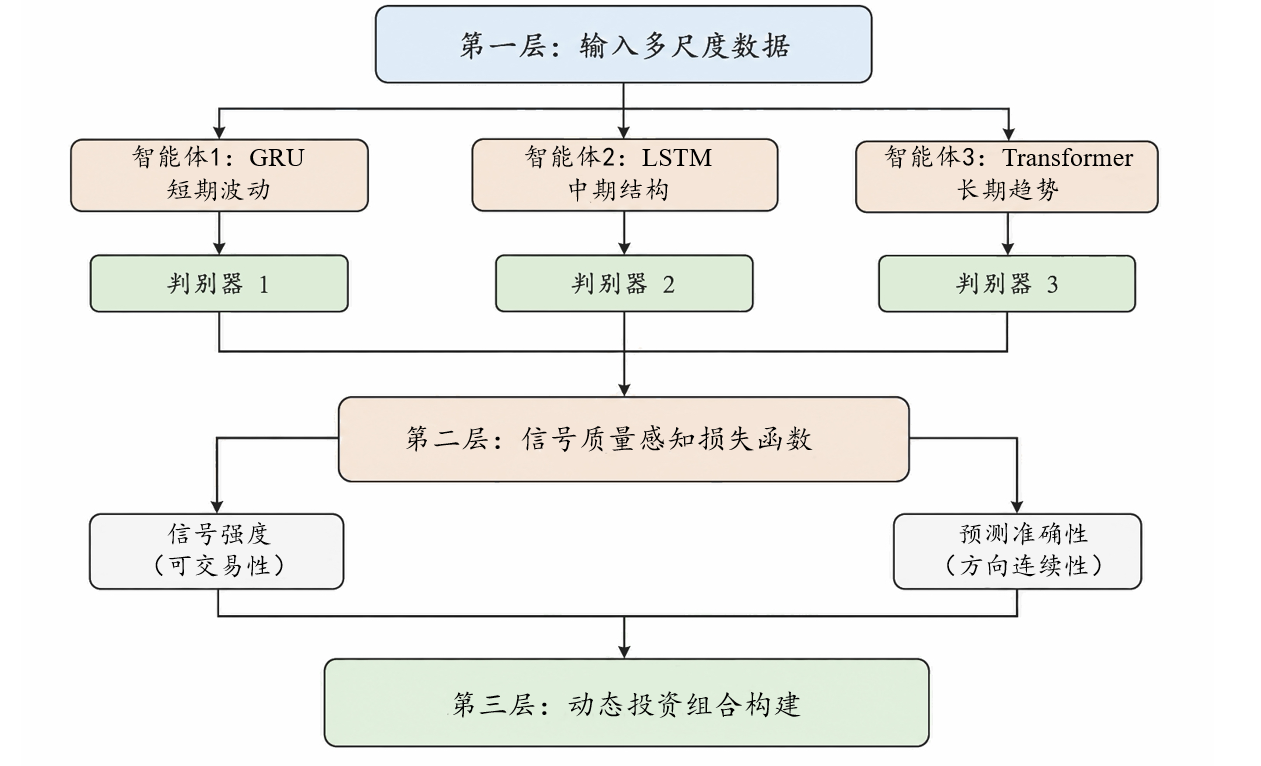
\includegraphics[width=0.8\textwidth]{figures/chap3/KDJ架构.png}
    \caption{GCA 多智能体群组交叉对抗整体框架示意图}
    \label{fig:MGCA-architecture}
\end{figure}

在这个多智能体系统中，GCA不再将多个模型视为静态集成，而是通过生成器与判别器之间的交叉评估来组织动态博弈。在真实金融市场中，算法交易已经深度影响市场流动性与交易过程，因而模型间交互不能简单视为静态预测器组合\cite{hendershott2011algorithmic}。在该系统中，多个异构生成器智能体基于各自的归纳偏置，对数据模式进行差异化刻画；多个判别器智能体则通过跨生成器的交叉评估机制，对生成结果在分布层面的合理性进行持续约束。生成器、判别器与元权重调节机制相互配合，共同推动多智能体系统向更加稳健的均衡状态演化。

形式化地，GCA核心机制由异构生成器集合$\mathcal{G}$与判别器集合$\mathcal{D}$构成：
\[
\mathcal{G} = \{G_1, G_2, \dots, G_N\}, \quad
\mathcal{D} = \{D_1, D_2, \dots, D_N\}.
\]
与经典生成对抗网络中“一对一”的生成器—判别器配对方式不同，本框架采用全连接的多对多博弈拓扑结构。通过引入端到端可微的元学习权重网络（Meta-weight Network），模型能够在训练过程中动态融合不同异构生成器输出，并调节子网络之间的相互作用强度，从而在多资产收益预测与组合权重生成之间建立更稳定的映射关系。


本章的整体方法对象是面向投资组合管理的GCA机制。GCA通过异构模型之间的交叉对抗学习，实现多尺度信息整合与分布正则化，避免模型趋同与模式崩塌，并将多模型输出进一步转化为投资组合管理所需的资产配置依据。为保持章节边界清晰，逆向师生蒸馏和孪生对抗自体再生在本章中不作为独立方法展开，也不被表述为本章的主体创新；它们仅作为GCA训练流程可接入的知识传递与状态修复接口，用于在消融实验中观察辅助机制对训练稳定性和组合表现的边际影响。
在这一结构中，多个异构智能体通过分组协同与交叉评估进行对抗学习，使生成器输出在数值精度和分布一致性之间形成约束。由此，本章方法的核心仍是“多资产预测信号如何转化为组合权重”，而不是提前展开后续章节的机制设计。

在上述整体架构下，本章进一步给出群组交叉对抗学习方法的训练流程。该流程包括初始化与预热、宏观演化与组间对抗、以及可选接口配置三个层次，分别对应模型启动、跨组竞争和辅助配置记录。这样安排的目的，是把GCA自身的训练主线和后续章节机制的接口位置区分开来，避免将本章写成多个创新模块的并列介绍。
GCA训练流程如算法 \ref{alg:MGCA_init}、\ref{alg:MGCA_evolution}、\ref{alg:MGCA_optional} 所示，其中GCA预热与组间对抗构成核心训练阶段，逆向师生蒸馏和孪生对抗自体再生仅作为可选辅助接口。

这里的“生成器”实际上充当的是“预测模型”的角色。将其称为“生成器”是为了将其纳入“对抗学习”的框架中，但其本质任务是条件预测。本文的核心目标不是生成逼真的假数据（如图像生成），而是生成鲁棒的投资组合权重。为了实现这一目标，模型需要先“生成”对未来收益的预测。在金融时序预测中，将模型视为生成器（生成未来的预测值）是一种常见的变通做法，尤其是在时间序列预测GAN的变体中。
判别器的输入是 (输入序列, 输出序列) 的组合。目标是判别器试图区分真实样本和生成样本。判别器的逻辑变为它不是在判断输出序列是真是假，而是在判断 “给定输入序列，输出序列这个组合是否符合真实市场的联合分布”。

结合上述分析，GCA 框架对生成器输出（预测收益率）的期待是双重的：
首先在数值上的准确性上，输出序列应该尽可能接近真实的未来收益率（由 LMSEL MSE保证）。
其次在分布上的一致性上（Distribution Consistency）：输出序列与输入 序列的联合分布应该无法与真实数据区分开（由 LadvL adv保证）。最终目标（Portfolio Management）是为了最终的夏普比率最大化（ LSharpeL Sharpe ）。文档 2.3.3 明确指出，优化目标是最大化夏普比率，这意味着模型不仅要预测方向，还要控制风险（波动率）。

\begin{algorithm}[H]
\caption{GCA 框架初始化与预热}
\label{alg:MGCA_init}
\begin{algorithmic}[0]
\Require 训练集 $\mathcal{D}_{\text{train}}$，验证集 $\mathcal{D}_{\text{val}}$；生成器集合 $\mathcal{G}$，判别器集合 $\mathcal{D}$
\Ensure 预热后的生成器集合 $\mathcal{G}$
\Statex
\State \textbf{初始化：} 随机初始化 $\mathcal{G}$ 和 $\mathcal{D}$，配置 Adam 优化器；创建多尺度滑动窗口数据集
\Statex
\State \textbf{Stage 1：组内交叉对抗（GCA）预热}
\For{epoch $= 1$ to $N_{\text{pretrain}}$}
    \For{each batch $(x^{(i)}, y) \in \mathcal{D}_{\text{train}}$, $i = 1 \ldots N$}
        \State 生成器前向：$\hat{y}_i \leftarrow G_i(x^{(i)})$
        \State \textbf{判别器训练：} 计算 $y$（标签 1）与 $\hat{y}_i$（标签 0）的二元交叉熵，更新 $D_i$
        \State \textbf{生成器训练：}
        \State $\quad \mathcal{L}_{\text{task}} \leftarrow \sum_{i=1}^N \lambda_i^{\text{task}} \cdot \text{MultiTaskLoss}(G_i(x^{(i)}), y)$
        \State $\quad \mathcal{L}_{\text{adv}} \leftarrow \sum_{i=1}^N \lambda_i^{\text{gan}} \cdot \left[-\log D_i(x^{(i)}, \hat{y}_i)\right]$
        \State $\quad \mathcal{L}_{\text{sharpe}} \leftarrow \lambda_{\text{sharpe}} \cdot \text{SharpeLoss}(\{\hat{y}_i\})$
        \State $\quad \mathcal{L}_G \leftarrow \lambda_{\text{mse}}\mathcal{L}_{\text{task}} + \lambda_{\text{gan}}\mathcal{L}_{\text{adv}} + \lambda_{\text{sharpe}}\mathcal{L}_{\text{sharpe}}$
        \State $\quad$ 使用 $\mathcal{L}_G$ 更新 $\mathcal{G}$
    \EndFor
\EndFor
\State \Return $\mathcal{G}$
\end{algorithmic}
\end{algorithm}

\begin{algorithm}[H]
\caption{GCA 框架宏观演化与组间对抗}
\label{alg:MGCA_evolution}
\begin{algorithmic}[0]
\Require 预热后的生成器集合 $\mathcal{G} = \{G_i\}$，判别器集合 $\mathcal{D} = \{D_i\}$，验证集 $\mathcal{D}_{\text{val}}$
\Ensure 全局最优生成器 $G^{\star}$
\Statex
\State \textbf{Stage 2：宏观演化循环 — 组内选拔与蒸馏}
\For{global\_epoch $= 1$ to $N_{\text{global}}$}
    \For{inner\_epoch $= 1$ to $N_{\text{inner}}$}
        \State 在 $\mathcal{D}_{\text{val}}$ 上评估：
        \State $\quad G_i^{\star} \leftarrow \arg\min_{G_i} \text{MSE}(G_i)$
        \State $\quad D_i^{\star} \leftarrow \arg\min_{D_i} \text{CE}(D_i)$
        \State 在组内执行一对一 生成对抗网络 对抗训练与知识蒸馏（蒸馏项：均方误差(Logits) + 均方误差(Features)）
    \EndFor
\EndFor
\Statex
\State \textbf{Stage 3：组间对抗 — 跨组竞争收敛}
\For{outer\_epoch $= 1$ to $N_{\text{outer}}$}
    \State 在 $\mathcal{D}_{\text{val}}$ 上选取最优生成器与判别器：
    \State $\quad G^{\dagger} \leftarrow \arg\min_{G_i^{\star}} \text{MSE}(G_i^{\star})$
    \State $\quad D^{\dagger} \leftarrow \arg\min_{D_i^{\star}} \text{CE}(D_i^{\star})$
    \State 在 $G^{\dagger}$ 与 $D^{\dagger}$ 之间执行组间 生成对抗网络 对抗训练
\EndFor
\Statex
\State 在 $\mathcal{D}_{\text{val}}$ 上评估：$G^{\star} \leftarrow \arg\min_G \text{MSE}(G)$
\State \Return $G^{\star}$
\end{algorithmic}
\end{algorithm}

\begin{algorithm}[H]
\caption{GCA 框架可选接口配置}
\label{alg:MGCA_optional}
\begin{algorithmic}[0]
\Require GCA训练输出 $G^{\star}$，候选生成器集合 $\{G_i\}$，验证集 $\mathcal{D}_{\text{val}}$
\Ensure 消融实验中的接口配置
\State 以GCA训练流程作为主配置，记录基准表现
\If{启用知识传递接口}
    \State 将该接口作为消融配置接入GCA训练结果
    \State 仅记录其对收益、回撤和换手率的边际影响；具体机制在后续章节展开
\EndIf
\If{启用状态修复接口}
    \State 将该接口作为消融配置接入GCA训练结果
    \State 仅记录其对模型稳定性和组合表现的边际影响；具体机制在后续章节展开
\EndIf
\State \Return 不同接口配置下的GCA模型结果
\end{algorithmic}
\end{algorithm}


在时间复杂度方面，算法1的单次迭代复杂度主要来源于生成器与判别器的前向传播和反向传播。设生成器/判别器的数量为 $N$，批次大小为 $B$，时间窗口长度为 $T$，隐藏层维度为 $d$，则单个生成器的前向传播复杂度为 $O(T^2 \cdot d)$（针对自注意力序列模型）或 $O(T \cdot d^2)$（针对循环神经网络架构）。综合考虑多生成器并行训练的场景，算法1每轮迭代的总时间复杂度为 $O(N \cdot B \cdot (T^2 \cdot d + T \cdot d^2))$。若预训练轮数为 $N_{\text{pretrain}}$，每轮包含 $N_{\text{batch}}$ 个批次，则算法1的总时间复杂度为 $O(N_{\text{pretrain}} \cdot N_{\text{batch}} \cdot N \cdot B \cdot (T^2 \cdot d + T \cdot d^2))$。在实际应用中，由于 $N_{\text{batch}} = |\mathcal{D}_{\text{train}}| / B$，该复杂度与训练集规模呈线性关系。

算法2在算法1的基础上增加了组内选拔蒸馏与组间对抗两个阶段。设组内蒸馏轮数为 $N_{\text{inner}}$，组间对抗轮数为 $N_{\text{outer}}$，全局演化轮数为 $N_{\text{global}}$。组内蒸馏阶段需要对每个生成器在验证集上进行评估，其复杂度为 $O(N \cdot |\mathcal{D}_{\text{val}}| \cdot (T^2 \cdot d + T \cdot d^2))$，随后执行的一对一生成对抗网络对抗训练与知识蒸馏的复杂度与算法1相当。组间对抗阶段仅对选出的最优生成器与判别器进行训练，其复杂度为 $O(N_{\text{outer}} \cdot B \cdot (T^2 \cdot d + T \cdot d^2))$，较组内阶段显著降低。因此，算法2的总时间复杂度约为 $O(N_{\text{global}} \cdot N_{\text{inner}} \cdot N \cdot |\mathcal{D}_{\text{val}}| \cdot (T^2 \cdot d + T \cdot d^2) + N_{\text{outer}} \cdot B \cdot (T^2 \cdot d + T \cdot d^2))$。验证集评估的复杂度在实际中通常低于训练前向传播，因为该过程无需进行梯度计算与参数更新。

算法3仅用于说明GCA训练流程可以接入知识传递与状态修复接口。逆向师生蒸馏和孪生对抗自体再生在本章中不作为独立展开的主体机制，而是作为消融实验中的可选配置，用于观察辅助接口在稳定训练和异常修复方面的边际作用。其具体算法细节将在后续章节结合相应任务展开。

在空间复杂度方面，以GCA为核心的多智能体对抗方法的主要存储开销包括模型参数存储、激活值存储、优化器状态存储以及数据存储四个部分。设单个生成器的参数量为 $|\theta_G|$，单个判别器的参数量为 $|\theta_D|$，则模型参数存储的空间复杂度为 $O(N \cdot (|\theta_G| + |\theta_D|))$。在前向传播过程中，需要存储各层的中间激活值用于反向传播，其空间复杂度为 $O(N \cdot B \cdot T \cdot d)$。若采用Adam优化器，需要为每个参数维护一阶矩和二阶矩，优化器状态的存储开销为模型参数的两倍，即 $O(2N \cdot (|\theta_G| + |\theta_D|))$。此外，训练数据和验证数据需要加载至内存，其空间复杂度为 $O(|\mathcal{D}_{\text{train}}| \cdot T \cdot F + |\mathcal{D}_{\text{val}}| \cdot T \cdot F)$，其中 $F$ 为特征维度。

从整体框架的复杂度特征来看，GCA训练流程的时间复杂度主要由算法1和算法2中的前向传播与反向传播决定，与生成器数量 $N$、训练集规模 $|\mathcal{D}_{\text{train}}|$ 以及模型深度 $(T^2 \cdot d)$ 呈线性或近似线性关系。空间复杂度则主要受模型参数量和批次大小影响。相较于传统的单生成器-单判别器生成对抗网络框架，该流程引入了 $N$ 倍的计算和存储开销，但通过并行化训练和验证集评估的优化，该开销在实际部署中处于可接受范围内。算法3中的可选接口只用于说明框架可扩展性，其细节不作为本章展开重点。







%\subsection{评估指标体系}

%为了全面量化多智能体群组交叉对抗框架在金融场景下的有效性，我们构建了一个涵盖收益性、风险性和交易成本的多维评估体系:

% \subsubsection{风险调整后收益}

%\paragraph{1.风险调整后收益}
%此类指标衡量单位风险敞口下的超额回报，是评估策略鲁棒性的核心标准。
 
%\begin{itemize}
   % \item \textbf{夏普比率 (Sharpe Ratio)}：定义为超额收益的期望与标准差之比。高夏普比率意味着策略位于有效前沿（Efficient Frontier）的更优位置。
   % \item \textbf{卡玛比率 (Calmar Ratio)}：定义为年化收益率与最大回撤之比，衡量策略在极端市场环境下的修复能力。
%\end{itemize}

% \subsubsection{绝对收益与稳定性特征}
%\paragraph{2.绝对收益与稳定性特征}
%\begin{itemize}
    %\item \textbf{年化收益率 (AnnRet)}：直观反映了策略的财富积累速度。
   % \item \textbf{最大回撤 (MDD)}：描述了资金曲线从峰值的最大跌幅，量化了策略的尾部风险。
%\end{itemize}

% \subsubsection{交易行为特征}
%\paragraph{3.交易行为特征}
%\begin{itemize}
    %\item \textbf{胜率 (Win Rate)}：盈利交易占比。
    %\item \textbf{平均换手率 (Average Turnover)}：反映了策略的交易频率。在考虑交易成本（Transaction Costs）和滑点（Slippage）的现实环境中，低换手率是防止利润被摩擦成本侵蚀的关键因素。
%\end{itemize}



上述说明限定了辅助接口在本章中的位置。后续实验以GCA为主方法，在统一回测框架下观察其对不同资产组合配置效果的影响，并在消融设置中报告辅助接口的边际作用。

\section{实验}

本节在统一的数据划分、回测规则与评价指标下检验GCA在投资组合管理任务中的表现。实验围绕“多资产收益预测—组合权重生成—风险收益评估”展开，重点观察GCA能否改善多资产配置中的风险调整后收益，并降低单一模型在不同市场状态下的配置偏差。因此，本节不把实验结果简单解释为预测精度提升，也不把辅助接口的边际效果上升为本章主体贡献，而是结合权重生成质量、回撤控制和组合层面表现分析GCA是否真正服务于投资组合管理。

为了将投资组合管理中的预测信号转化为可执行的资产权重，我们将生成器的输出通过稳健的策略函数转化为实际仓位。早期交易系统研究已经指出，交易模型应直接围绕投资绩效函数进行优化，而不仅是最小化预测误差\cite{moody1998performance}。这一观点与本章方法目标一致：模型输出只有转化为仓位并接受收益、风险和交易约束检验，才具有投资组合管理意义。

本章采用连续多空策略，将预测信号映射为资产权重。直接强化学习交易研究表明，将预测信号直接映射为交易动作或仓位决策，有助于弥合统计预测与交易执行之间的距离\cite{moody2001learning}：
\begin{equation}
    w_{i,t} = \frac{\hat{r}_{i,t} - \bar{r}_t}{\sum_{j} |\hat{r}_{j,t} - \bar{r}_t|}
\end{equation}
其中 $\bar{r}_t$ 为截面均值。该策略实现了资金的中性化配置（Dollar Neutral），即 $\sum w_{i,t} = 0$，专注于捕捉资产间的相对强弱关系（阿尔法），而非市场的系统性风险（贝塔）。

%\subsection{交易执行与回测框架}

为说明模型输出如何进入样本外回测，本文采用统一的交易执行与回测框架。算法交易研究强调，预测信号只有在执行机制与市场微观结构约束下转化为真实订单后，才具有完整的经济意义\cite{cartea2015algorithmic}。模型生成的分类预测经 softmax 归一化后得到三类信号概率 $(p_0, p_1, p_2)$，分别对应做空、持有、做多的概率。取 $\max(p_0, p_2)$ 作为置信度权重 $w_t \in [0,1]$，再根据预测类别 $a$ 确定方向，计算策略每日收益率：
\[
w_t = \max(p_0, p_2), \qquad
r_t^{\text{strategy}} =
\begin{cases}
  +w_t \cdot r_t, & a = 2 \text{（做多）} \\
  -w_t \cdot r_t, & a = 0 \text{（做空）} \\
  0, & a = 1 \text{（持有）}
\end{cases}
\]
其中 $r_t = (P_t - P_{t-1}) / P_{t-1}$ 为基础价格变化率。策略不涉及保证金制度或杠杆，$w_t$ 即为实际名义敞口比例（最大为 1，即满仓）。

\textbf{Equity 曲线与累计收益}：Equity 曲线以 $1.0$ 为起点，通过逐日复利累乘计算：
\[
\text{equity}_t = \prod_{i=1}^{t}\left(1 + r_i^{\text{strategy}}\right).
\]
累计收益率和年化收益率即在此 equity 曲线的基础上计算得到。

\textbf{投资策略评估指标}：为评估交易策略在样本外回测中的表现，本框架采用包含风险、收益和交易摩擦的多维指标体系：
\begin{itemize}
    \item \textbf{风险调整后收益}：\textbf{夏普比率}，用于衡量单位风险下的超额收益能力。夏普关于基金绩效评价的经典研究为风险调整收益度量提供了早期依据\cite{sharpe1966mutual}。
    \item \textbf{收益表现}：\textbf{总收益率} 和 \textbf{年化收益率}。
    \item \textbf{风险控制}：\textbf{年化波动率} 和 \textbf{最大回撤}，以评估策略的稳定性与尾部风险。
    \item \textbf{交易特征}：\textbf{胜率} 和 \textbf{平均换手率}，用于反映信号的准确度及策略的交易成本敏感性。
\end{itemize}
此外，通过累计收益率曲线展示不同模型在样本外测试期间的净值变化和回撤修复情况。





%\section{实验数据与评估指标}

%\subsection{数据与实验设置}



%\subsection{实验数据与评估指标}
%\subsection{组合指数的构建}


%\subsubsection{QR 指标的定义}

%\subsubsection{实验组合设计}

% \section{实验组合设计}
为检验GCA机制在不同市场结构下的投资组合管理能力，本章以多资产组合配置作为实验对象，基于经济板块逻辑与资产间的相关性结构，构建了六类具有差异化市场特征的投资组合（P1--P6），如表~\ref{tab:portfoliosAligned}所示。该实验设计的目的不是验证单一资产预测效果，而是观察GCA在不同资产相关结构、不同数据长度和不同波动环境下，能否保持相对稳定的权重生成能力与风险调整收益表现：

% \begin{itemize}
%     \item \textbf{P1：宏观敏感型组合}（黄金、原油、铜、豆粕）——涵盖贵金属、能源与农产品，资产间受宏观经济周期与地缘政治事件驱动，旨在检验模型对突发状态切换的适应能力。
%     \item \textbf{P2：农产品周期组合}（玉米、豆粕、白糖、棉花）——受季节性供需与自然因素影响，具有显著的周期性与均值回归特征，用于验证模型对长期依赖的捕捉能力。
%     \item \textbf{P3：能源-化工链条组合}（原油、甲醇、聚丙烯、PTA）——上下游产业链资产，存在因果时滞与波动率传导效应，用于测试模型对跨资产价格传导的结构化推理能力。
%     \item \textbf{P4：避险-风险对冲组合}（黄金、铜、原油、动力煤）——包含避险资产与周期性风险资产，在不同市场状态下呈现动态变化的相关结构，用于验证模型的多目标优化与动态对冲能力。
%     \item \textbf{P5：高波动技术交易组合}（PVC、甲醇、PTA、聚丙烯）——均为波动率较高的化工品种，收益分布呈厚尾特征，用于压力测试模型在极端行情下的风险适应性。
%     \item \textbf{P6：多元低相关组合}（黄金、棉花、铁矿石、白糖、动力煤）——跨越多个独立板块，资产间相关性较低，用于测试模型在低信噪比环境下的特征解耦能力与防过拟合能力。
% \end{itemize}

% {P1}是宏观敏感型组合（黄金、原油、铜、豆粕），这一类主要涵盖贵金属、能源与农产品，资产间受宏观经济周期与地缘政治事件驱动，旨在检验模型对突发状态切换的适应能力；
% {P2}是农产品周期组合（玉米、豆粕、白糖、棉花），这一类受季节性供需与自然因素影响，具有显著的周期性与均值回归特征，用于验证模型对长期依赖的捕捉能力；
% {P3}是能源-化工链条组合（原油、甲醇、聚丙烯、PTA），存在明显时滞与波动率传导效应，用于测试模型对跨资产价格传导的结构化推理能力；
% {P4}为避险-风险对冲组合（黄金、铜、原油、动力煤），资产在不同市场状态下呈现动态变化，以验证模型的多目标优化与动态对冲能力；
% {P5}为高波动技术交易组合（PVC、甲醇、PTA、聚丙烯），由波动率较高的化工品种组成，收益分布呈厚尾特征，用于压力测试模型在极端行情下的风险适应性；
% {P6}为多元低相关组合（黄金、棉花、铁矿石、白糖、动力煤），用于检验模型在低信噪比环境下的特征解耦能力与防过拟合能力。


上述组合在驱动因素、波动特征、相关结构及数据长度等维度上形成互补，用于观察GCA机制在宏观事件冲击、产业链传导、周期性波动及极端市场环境下的资产配置能力和组合风险控制能力。具体的资产配置与有效回测区间如表 \ref{tab:portfoliosAligned} 所示。

\begin{table}[htbp]
    \centering
    \caption{实验资产组合配置与有效对抗训练区间}
    \label{tab:portfoliosAligned}
    \resizebox{\textwidth}{!}{%
    \begin{tabular}{clll}
    \toprule
    \textbf{编号} & \textbf{组合名称} & \textbf{底层资产} & \textbf{有效区间} \\
    \midrule
    P1 & 宏观敏感型组合 & Gold, Crude Oil*, Copper, Soybean Meal & 2018.03 - 2024.12 \\
    P2 & 农产品核心组合 & Corn, Soybean Meal, Sugar, Cotton & 2006.01 - 2024.12 \\
    P3 & 能源-化工联动组合 & Crude Oil*, Methanol, PP, PTA & 2018.03 - 2024.12 \\
    P4 & 避险-风险对冲组合 & Gold, Copper, Crude Oil*, Thermal Coal & 2018.03 - 2024.12 \\
    P5 & 高波动技术交易组合 & PVC, Methanol, PTA, PP & 2014.02 - 2024.12 \\
    P6 & 多元低相关组合 & Gold, Cotton, Iron Ore, Sugar, Thermal Coal & 2013.10 - 2024.12 \\
    \bottomrule
    \end{tabular}%
    }
    \begin{tablenotes}
        \footnotesize
        \item[*] 注：带 * 号资产（如原油 SC）为该组合的“时间瓶颈”资产，限制了整体回测的起始点。这种差异化的时间窗口恰好允许我们评估模型在长周期（如 P2）与短周期（如 P1）不同数据丰度下的鲁棒性。
    \end{tablenotes}
\end{table}

该组合设计从三方面体现验证价值：一是数据丰度适应性检验上，P2近20年的完整周期数据可用于验证模型的收敛上限，P1、P4约6年数据用于测试小样本泛化能力；二是逻辑合理性，通过P3组合验证模型对产业链价格传导的捕捉能力；三是环境鲁棒性，利用P5高波动组合实现极端行情下的模型压力测试。

\subsection{实验数据集}
为服务多资产投资组合管理任务，本章构建了一个高维特征输入空间，用于同时刻画各资产自身的量价状态、资产之间的相对强弱关系以及组合配置所需的风险收益信息。金融深度学习基准研究表明，量价序列、订单流与技术指标等多维特征对于刻画市场微观结构具有重要意义\cite{ntakaris2018benchmark}。数据集不仅包含基础的量价数据（开盘价、最高价、最低价、收盘价与成交量），还通过特征工程构建了三大类技术指标：
% \begin{enumerate}
%     \item \textbf{趋势类指标}：包括多周期移动平均（MA5/15/30）与指数平滑异同移动平均（MACD），用于捕捉截面动量；
%     \item \textbf{震荡类指标}：包括相对强弱指数（RSI）与随机指标（KDJ），用于识别超买超卖的市场状态；
%     \item \textbf{波动类指标}：包括真实波幅（ATR）与布林带（Bollinger Bands），用于量化市场的不确定性边界。
% \end{enumerate}
趋势类指标包括多周期移动平均（MA5/15/30）与指数平滑异同移动平均线，用于捕捉截面动量；
震荡类指标包括相对强弱指数与随机指标，用于识别超买超卖的市场状态；
波动类指标包括真实波幅与布林带，用于量化市场的不确定性边界。

数据集的特征池包括：
\begin{itemize}
   
    \item 价格和成交量：开盘价、最高价、最低价、收盘价、平均价和成交量。
   
    \item 持仓量：当前未平仓且未结算或关闭的衍生品合约（期货或期权）总数。
    
    \item 移动平均线因子：5日、15日和30日简单移动平均线（MA5、MA15、MA30）。
   
    \item 差离值：12日和26日指数移动平均线之间的差值。
   
    \item 信号线：差离值的9日指数移动平均线。
 
    \item 指数平滑异同移动平均线：计算为 差离值 减去 信号线，反映趋势强度和方向。
    
    \item 真实波幅：14日窗口内的平均真实波幅，捕捉价格波动性。
   
    \item 布林带：使用20日移动平均线和2倍标准差构建，用于指示相对价格水平。
   
    \item 相对强弱指数：基于14日周期计算，用于捕捉动量。
    
    \item K, D, J：随机指标（Stochastic Oscillator）分量，捕捉价格动量和反转信号，其中 K 是9日随机值，D 是其3日移动平均值，J 是动量乖离。
\end{itemize}
所有特征在输入神经网络前均经过严格的 区间缩放标准化 处理。我们为每个资产 $i$ 的每个特征 $f$ 独立计算训练集的极值，将其映射至 $[0, 1]$ 区间：
\begin{equation}
    x^{(i,f)}_{norm} = \frac{x^{(i,f)} - \min(X_{train}^{(i,f)})}{\max(X_{train}^{(i,f)}) - \min(X_{train}^{(i,f)})}
\end{equation}
这种处理有效消除不同指标（如价格的 $10^3$ 量级与 指数平滑异同移动平均线 的 $10^{-1}$ 量级）之间的尺度差异，确保梯度下降过程的各向同性。
% \subsection{实验参数设置}
\subsection{实验设计}
为了捕捉多尺度的时间动态并获取宏观视野，本文采用5、10 、20三种递增的输入窗口，分别对应周度脉冲、双周度波段和月度结构特征。
数据预处理阶段，为了消除量纲差异并加速梯度收敛，对上述特征采用了区间缩放标准化，将其映射至 $[0, 1]$ 区间：
\begin{equation}
    x_{norm} = \frac{x - x_{min}}{x_{max} - x_{min}}
\end{equation}
其中统计量 $x_{min}, x_{max}$ 仅在训练集上计算，以严格避免前瞻性偏差。

数据集按照时间顺序进行划分，将前70\%的数据作为训练集用于优化模型参数，后30\%的数据作为测试集用于样本外评估。本章之所以不采用随机打乱划分，是因为投资组合管理任务具有明确的时间先后关系，模型在测试阶段只能利用历史信息形成预测与权重配置，而不能提前接触未来样本。金融回测研究表明，多重检验、过度试验和样本外失效是量化策略评估中需要重点防范的问题\cite{harvey2016backtesting}。对于本文而言，这一问题尤其需要注意，因为本章同时比较多类模型、输入窗口和消融配置，若实验设计缺少统一约束，局部最优结果可能被误判为方法本身的稳定优势。

在多模型比较场景中，若研究者反复尝试不同模型、参数或组合设定，容易出现由数据窥探导致的偶然优胜。White的Reality Check从数据窥探角度讨论了多模型检验下的偶然优胜风险\cite{white2000realitycheck}。这一思想提示本文，模型比较不能只关注某个配置在测试集上的最高收益，而应在统一数据划分、统一交易规则和统一评价指标下观察不同模型的整体表现。Hansen提出的superior predictive ability检验进一步针对预测模型比较中的数据窥探问题提出了改进方案\cite{hansen2005spa}。因此，本章在实验设计中尽量固定数据划分、输入窗口和评估指标，使模型差异主要来自方法结构本身，而不是来自反复试验带来的选择偏差。

此外，回测过拟合研究从投资策略选择角度说明，标准留出法并不总能充分识别样本外失效风险\cite{bailey2015pbo}。基于这一考虑，本文在训练集与测试集之间设置长度为 $L_{gap}=20$ 天（即最大输入窗口长度）的“隔离期”。该期间数据不参与梯度更新与回测评估，用于减少训练末期窗口信息对测试初期样本的干扰，从而在不改变原始时间顺序的前提下，降低前瞻性偏差对实验结论的影响。

\noindent\textbf{评价指标说明}\par
本章在样本外测试中统一采用风险调整后收益、收益表现、风险控制与交易特征四类指标。具体包括夏普比率、卡玛比率、累计收益率、年化收益率、年化波动率、最大回撤、胜率和平均换手率。其中，夏普比率与卡玛比率用于衡量单位风险下的收益能力，累计收益率与年化收益率反映绝对收益水平，年化波动率与最大回撤刻画风险暴露，胜率与平均换手率用于观察交易信号质量及交易摩擦敏感性。



\noindent\textbf{消融与对照组实验设计}\par
% \subsection{添加交叉对抗后的性能退化验证}

% 为全面验证各模块的独立贡献与交互效应，本章采用两条消融路径并行的策略。

本章构建统一消融实验基准，重点检验GCA在投资组合管理任务中的作用。除基准模型与GCA配置外，实验仅保留知识传递接口和状态修复接口两类辅助配置，用于观察它们对GCA训练稳定性和组合表现的边际影响。相关接口不在本章展开机制细节，其作用仅通过消融实验进行报告。

% 路径B的核心目的，是在各章应用语境中验证本章主要贡献确实解决了本章声称的问题，避免固定场景带来的偏差。该路径通过渐进式消融实验，逐项验证各机制的有效性。

% 本章节渐进消融表（6-7行）：
\begin{table}[htbp]
\centering
\caption{渐进消融实验}
\label{tab:ablation_chap3_local}
\small
\setlength{\tabcolsep}{6pt}
\renewcommand{\arraystretch}{1.18}
\begin{tabular}{@{}p{0.36\textwidth}ccc@{}}
\toprule
\textbf{实验} & \textbf{GCA} & \textbf{知识传递接口} & \textbf{状态修复接口} \\
\midrule
基准模型 & $\times$ & $\times$ & $\times$ \\
+ GCA & $\checkmark$ & $\times$ & $\times$ \\
+ GCA+知识传递接口 & $\checkmark$ & $\checkmark$ & $\times$ \\
+ GCA+知识传递接口+状态修复接口 & $\checkmark$ & $\checkmark$ & $\checkmark$ \\
\bottomrule
\end{tabular}
\end{table}

% 关键交互对比（3个）：
% \begin{itemize}
%     \item GCA+S2T：验证交叉对抗是否需要双向蒸馏配合
%     \item S2T+Twin：验证逆向师生蒸馏是否需要孪生对抗自体再生配合
% \end{itemize}

% \textbf{修正说明}：第3章使用三个主要贡献（GCA+S2T+Twin），消融实验验证各模块的独立贡献。

% 输出策略：正文展示路径B（叙事贴合痛点），附录给出路径A（提供统一基准与交互效应解释）

% \begin{table}[htbp]
% \centering
% \caption{消融实验结果汇总表}
% \label{tab:ablation_study}
% \resizebox{\textwidth}{!}{
% \begin{tabular}{cccccccc}
% \toprule
% \textbf{模块配置} & \textbf{夏普比率} & \textbf{总收益率} & \textbf{年化收益率} & \textbf{最大回撤} & \textbf{说明} \\
% \midrule
% Baseline & 0.22 & 13.64\% & 2.81\% & -27.60\% & 基线模型 \\
% GCA (无蒸馏) & 0.25 & 15.85\% & 3.27\% & -26.41\% & 去除组内/全局蒸馏 \\
% GCA+蒸馏 & 0.33 & 21.44\% & 4.42\% & -25.67\% & 去除交叉对抗 \\
% 完整 MGCA & 0.45 & 28.87\% & 5.95\% & -20.34\% & 完整框架 \\
% \bottomrule
% \end{tabular}}
% \end{table}

% \vspace{1em}
% \textit{注：消融实验在 P1 组合上验证各模块的独立贡献。}

% \subsection{多目标损失配置}

% \begin{table}[htbp]
% \centering
% \caption{多目标损失配置对比实验结果}
% \label{tab:loss_config_comparison}
% \resizebox{\textwidth}{!}{
% \begin{tabular}{cccccccc}
% \toprule
% \textbf{损失配置} & \textbf{夏普比率} & \textbf{累计收益} & \textbf{年化波动} & \textbf{最大回撤} & \textbf{说明} \\
% \midrule
% 仅 MSE & — & — & — & — & 基准配置 \\
% MSE + GAN & — & — & — & — & 加入对抗损失 \\
% MSE + Sharpe & — & — & — & — & 加入夏普损失 \\
% MSE + GAN + Sharpe (完整) & — & — & — & — & 完整配置 \\
% \bottomrule
% \end{tabular}}
% \end{table}

% \vspace{1em}
% \textit{注：多目标损失配置对比实验在 P2 组合上进行。}

训练采用渐进式消融实验验证各模块的增量贡献：
% \begin{enumerate}
%     \item 基准配置（Baseline）：采用单一的均方误差（MSE）作为损失函数，仅从统计层面约束预测的数值精度。
%     \item MGCA完整配置：在保留 MSE 作为基础锚点的同时，叠加了对抗损失（GAN Loss） 与 夏普比率损失（Sharpe Ratio Loss）。这种混合范式实现了三重优化：MSE 保证基础保真度，GAN 正则化防止过拟合，夏普损失则直接优化投资组合的风险调整后收益，从而在保证信号物理意义的同时最大化决策效用。
% \end{enumerate}
基准配置以单一均方误差作为损失函数，并从门控循环单元、长短期记忆网络和自注意力序列模型中选取最优模型作为对照；随后加入GCA，观察群组交叉对抗对投资组合配置效果的影响；最后仅以接口形式接入知识传递和状态修复配置，用于观察辅助机制的边际作用。

为比较GCA及其辅助配置的边际作用，本章设计三层对照组：

\textbf{第一层：单模型基线（验证单模型的局限性）}
% \begin{itemize}
%     \item GRU：门控循环单元
%     \item LSTM：长短期记忆网络
%     \item Transformer：自注意力机制
% \end{itemize}
分别训练门控循环单元，长短期记忆网络和自注意力序列模型对比其性能优劣以选取最优基线模型。


% \textbf{第二层：传统机器学习方法}
% \begin{itemize}
%     \item Random Forest：随机森林
%     \item XGBoost：梯度提升树
%     \item LightGBM：轻量级梯度提升
%     \item SVM：支持向量机
% \end{itemize}



\textbf{第二层：传统集成（验证传统集成的局限性）}
% \begin{itemize}
%     % \item Bagging：Bootstrap聚合的多个GRU
%     \item 简单平均：GRU+LSTM+Transformer的元学习集成
%     % \item AdaBoost：自适应提升
% \end{itemize}
使用简单平均的集成方法，门控循环单元+长短期记忆网络+自注意力序列模型的元学习集成以作为对比的基准模型。

\textbf{第三层：本章方法变体（验证各模块的边际贡献）}
分别是基准模型、基准模型+GCA、基准模型+GCA+知识传递接口，以及基准模型+GCA+知识传递接口+状态修复接口。该渐进式设置用于观察GCA核心机制及其辅助接口对组合配置流程的边际影响。
% \begin{itemize}
%     \item GCA：baseline+群组交叉对抗
%     \item GCA+S2T：群组交叉对抗+逆向师生蒸馏
%     \item GCA+S2T+Twin：前两者+孪生对抗自体再生
% \end{itemize}
% \textbf{第四层：多智能体基线（验证现有智能体框架的局限性）}
% \begin{itemize}
%     \item Multi-Agent RL（如MAPS）\cite{jiang2017deep}：独立训练的多智能体强化学习
%     \item DML \cite{zhang2018dml}：双向互学习（无对抗机制）
%     \item 标准GAN：单生成器单判别器
% \end{itemize}

% \textbf{第五层：GAN变种基线（验证 GAN 变体的局限性，基于文献综述[1]）}
% \begin{itemize}
%     \item \textbf{WGAN-GP}：Wasserstein GAN with Gradient Penalty，解决模式崩塌问题
%     \item \textbf{TTUR}：Two Time-Scale Update Rule，两时间尺度更新规则
%     \item \textbf{MGAN}：Multi-Generator GAN，多生成器+共享判别器，鼓励生成器学习不同模式
%     \item \textbf{MGO-GAN}：正交正则化去相关，强制生成器特征独立
%     \item \textbf{D2GAN}：Dual Discriminator GAN，双判别器（标准KL+反向KL）平衡质量与多样性
%     \item \textbf{Parallel Generators}：并行结构生成器，多生成器并行训练
%     \item \textbf{TimeGAN}：时序生成对抗网络，专门针对时间序列
%     \item \textbf{QuantGAN}：金融时间序列生成对抗网络
% \end{itemize}



% \textbf{公平性约束}：所有基线必须严格遵守同一backbone、同一训练预算、同一数据划分、同一seed集合，否则对照结论会被质疑。

% 参考文献：
% [1] 在生成对抗网络（GAN）训练中故意打破平衡：一项文献综述. AMiner, 2026.

% \section{可视化验证实验}

% % 为验证 多智能体群组交叉对抗框架是否真正解决了上述"静态权重失效"和"模型趋同"问题，本章设计了以下可视化验证实验。
% 为验证 多智能体群组交叉对抗框架是否有效及各模块的作用，本章设计了以下可视化验证实验。

% \vspace{0.3em}
% \noindent\textbf{实验1：模型多样性验证（针对"模型趋同"问题）}

% 目的：验证 GCA 对抗机制能否产生多样化的预测，避免模型趋同。

% % 方法：使用 t-SNE 方法对各生成器（GRU、LSTM、Transformer）的预测结果进行可视化降维，观察其分布差异。
% 方法：对各生成器（GRU、LSTM、Transformer）的预测结果进行可视化降维，观察其分布差异。

% 预期：经过 GCA 对抗训练后，各生成器的预测分布应更加分散，表明每个生成器学习到了不同的市场特征。

% % \vspace{0.3em}
% % \noindent\textbf{实验2：动态权重有效性验证（针对"静态权重"问题）}

% % 目的：验证元权重网络能否自适应市场状态。

% % 方法：绘制权重热力图，对比不同市场阶段（高波动期/低波动期）的权重分布。

% % 预期：在高波动期，Transformer 等擅长趋势建模的生成器权重应增加；在低波动期，GRU/LSTM 等擅长均值回归的生成器权重应增加。

% \vspace{0.3em}
% \noindent\textbf{实验2：知识蒸馏效果验证（针对"知识传承"问题）}

% 目的：验证蒸馏机制能否加速弱模型学习。

% 方法：绘制训练收敛曲线，对比有无蒸馏的模型性能差异。

% 预期：加入蒸馏后，落后的生成器应能更快收敛，且最终性能更高。

% \vspace{0.3em}
% \noindent\textbf{实验3：孪生对抗自体再生对比}

% 目的：验证孪生对抗自体再生机制能否改善预测效果。

% 方法：对比训练前后有无孪生对抗自体再生的模型性能差异。

% 预期：经过对抗训练后，模型输出的效果及回测结果展示应有明显改善。


\subsection{结果分析与讨论}
\noindent\textbf{GCA模型多样性验证}\par
% \begin{table}[htbp]
% \centering
% \caption{实验结果汇总表}
% \label{tab:experimental_results_summary}
% \resizebox{\textwidth}{!}{
% \begin{tabular}{cccccccc}
% \toprule
% \textbf{组合} & \textbf{模型} & \textbf{夏普比率} & \textbf{总收益} & \textbf{年化收益} & \textbf{最大回撤 } & \textbf{胜率} & \textbf{换手率}\\
% \midrule

% \multirow{5}{*}{\textbf{P1}} 
% &Baseline&0.2168  &13.64\% &2.81\%  & -27.60\% &49.63\% &0.0760\\
% &Baseline-GCA& 0.2474 & 15.85\% &  3.27\% & -26.41\% &49.63\% &0.0713\\ 
% &Baseline-GCA-S2T &-&-&-&-&-&-\\
% &Baseline-GCA-S2T-Twin&-&-&-&-&-&-\\
% \midrule
% \multirow{5}{*}{\textbf{P2}} 
% &Baseline &0.3652 & 60.61\% &3.64\% &-21.17\% &50.14\% &0.1538\\
% &Baseline-GCA&-0.1990 & -16.40\% & -0.99\% & -33.07\% & 49.9\% & 0.1859\\
% &Baseline-GCA-S2T & 0.6279 &105.73\% &6.35\% &-17.13\% & 51.03\% &0.0479\\
% &Baseline-GCA-S2T-Twin&0.6446 &108.61\% &6.53\%  &-16.51\% &50.86\% &0.0397\\
% \midrule
% \multirow{5}{*}{\textbf{P3}} 
% &Baseline &-0.2816 &-12.51\% & -2.58\%  &-31.25\% &48.41\% &0.1600 \\
% &Baseline-GCA& -0.0976 & -6.53\% & -1.35\%& -22.23\% & 48.98\% & 0.1220\\
% &Baseline-GCA-S2T&0.1936 &12.82\% &2.64\% &-17.54\% &49.71\% & 0.0838 \\
% &Baseline-GCA-S2T-Twin&0.5764 &38.91\% &8.02\% &-13.72\% &50.12\% & 0.0408\\
% \midrule
% \multirow{5}{*}{\textbf{P4}} &Baseline&  0.6926&40.33\% &15.31\% &-25.67\% & 49.70\% & 0.1287 \\
% &Baseline-GCA & 0.4158 & 24.14\% &  9.16\% & -29.29\% & 49.4\% &0.1164\\
% &Baseline-GCA-S2T&0.6814 &39.49\% &14.99\% &-24.23\% &48.49\% & 0.0638 \\
% &Baseline-GCA-S2T-Twin&0.7120&40.45\% &15.35\% &-23.95\% & 47.89\% & 0.0408\\
% \midrule
% \multirow{5}{*}{\textbf{P5}} &Baseline&-&-&-&-&-&-\\
% &Baseline-GCA &-0.2657 & -17.40\% & -1.98\% & -34.01\% & 48.96\% & 0.3665\\
% &Baseline-GCA-S2T&-&-&-&-&-&-\\
% &Baseline-GCA-S2T-Twin&-&-&-&-&-&-\\
% \midrule
% \multirow{5}{*}{\textbf{P6}} &Baseline&0.4917 &45.72\% &6.59\% &-16.17\% &52.00\% &0.0939\\
% &Baseline-GCA &0.3817 &35.09\% &5.06\% &-18.31\% & 51.32\% & 0.1120\\
% &Baseline-GCA-S2T&0.5613 &52.00\% &7.50\% &-13.61\% &51.37\% & 0.0751   \\
% &Baseline-GCA-S2T-Twin& 0.5234& 49.12\% & 7.08\% &-13.97\% &50.97\% & 0.0835\\

% \bottomrule
% \end{tabular}}
% \end{table}

% \vspace{1em}
% \textit{注：表中数据为样本外测试集结果，"—"表示未适用。}

为评估GCA架构在不同组合上的样本外表现，本节对比其与单一生成器基准模型（门控循环单元、长短期记忆网络、自注意力序列模型）在六大组合上的样本外性能，所有模型采用相同超参数，评价指标覆盖投资回报、风险控制与交易摩擦成本。这里的结果分析重点在于说明群组交叉对抗架构能否在不同市场结构下保持多智能体协同与风险约束能力，而不是单纯比较某一组合的收益高低。因此，以下分析将训练收敛性、组合层回测结果和权重动态变化放在同一评价框架中讨论。

% \subsubsection{模型训练收敛性分析}

为了探究异构模型在复杂金融流形上的优化效率，记录各模型在所有六个实验组合上的训练损失演化轨迹。图 \ref{MGCA框架的MSE训练损失图}、 \ref{GRU的MSE训练损失图}、 \ref{LSTM的MSE训练损失图}、 \ref{Transformer的MSE训练损失图}  展示了各模型均方误差项的收敛全过程。四幅图中六个子图的排列顺序保持一致，均按从左至右、从上至下依次对应 P1--P6 六类实验组合。
\begin{figure}[htbp] % [htbp] 是位置参数：这里(h)、页首(t)、页尾(b)、单独一页(p)
    \centering % 图片居中
    % width=\textwidth 表示图片宽度占满正文文本宽度
    % 如果在文件夹里，路径要是 figures/my_chart.png
    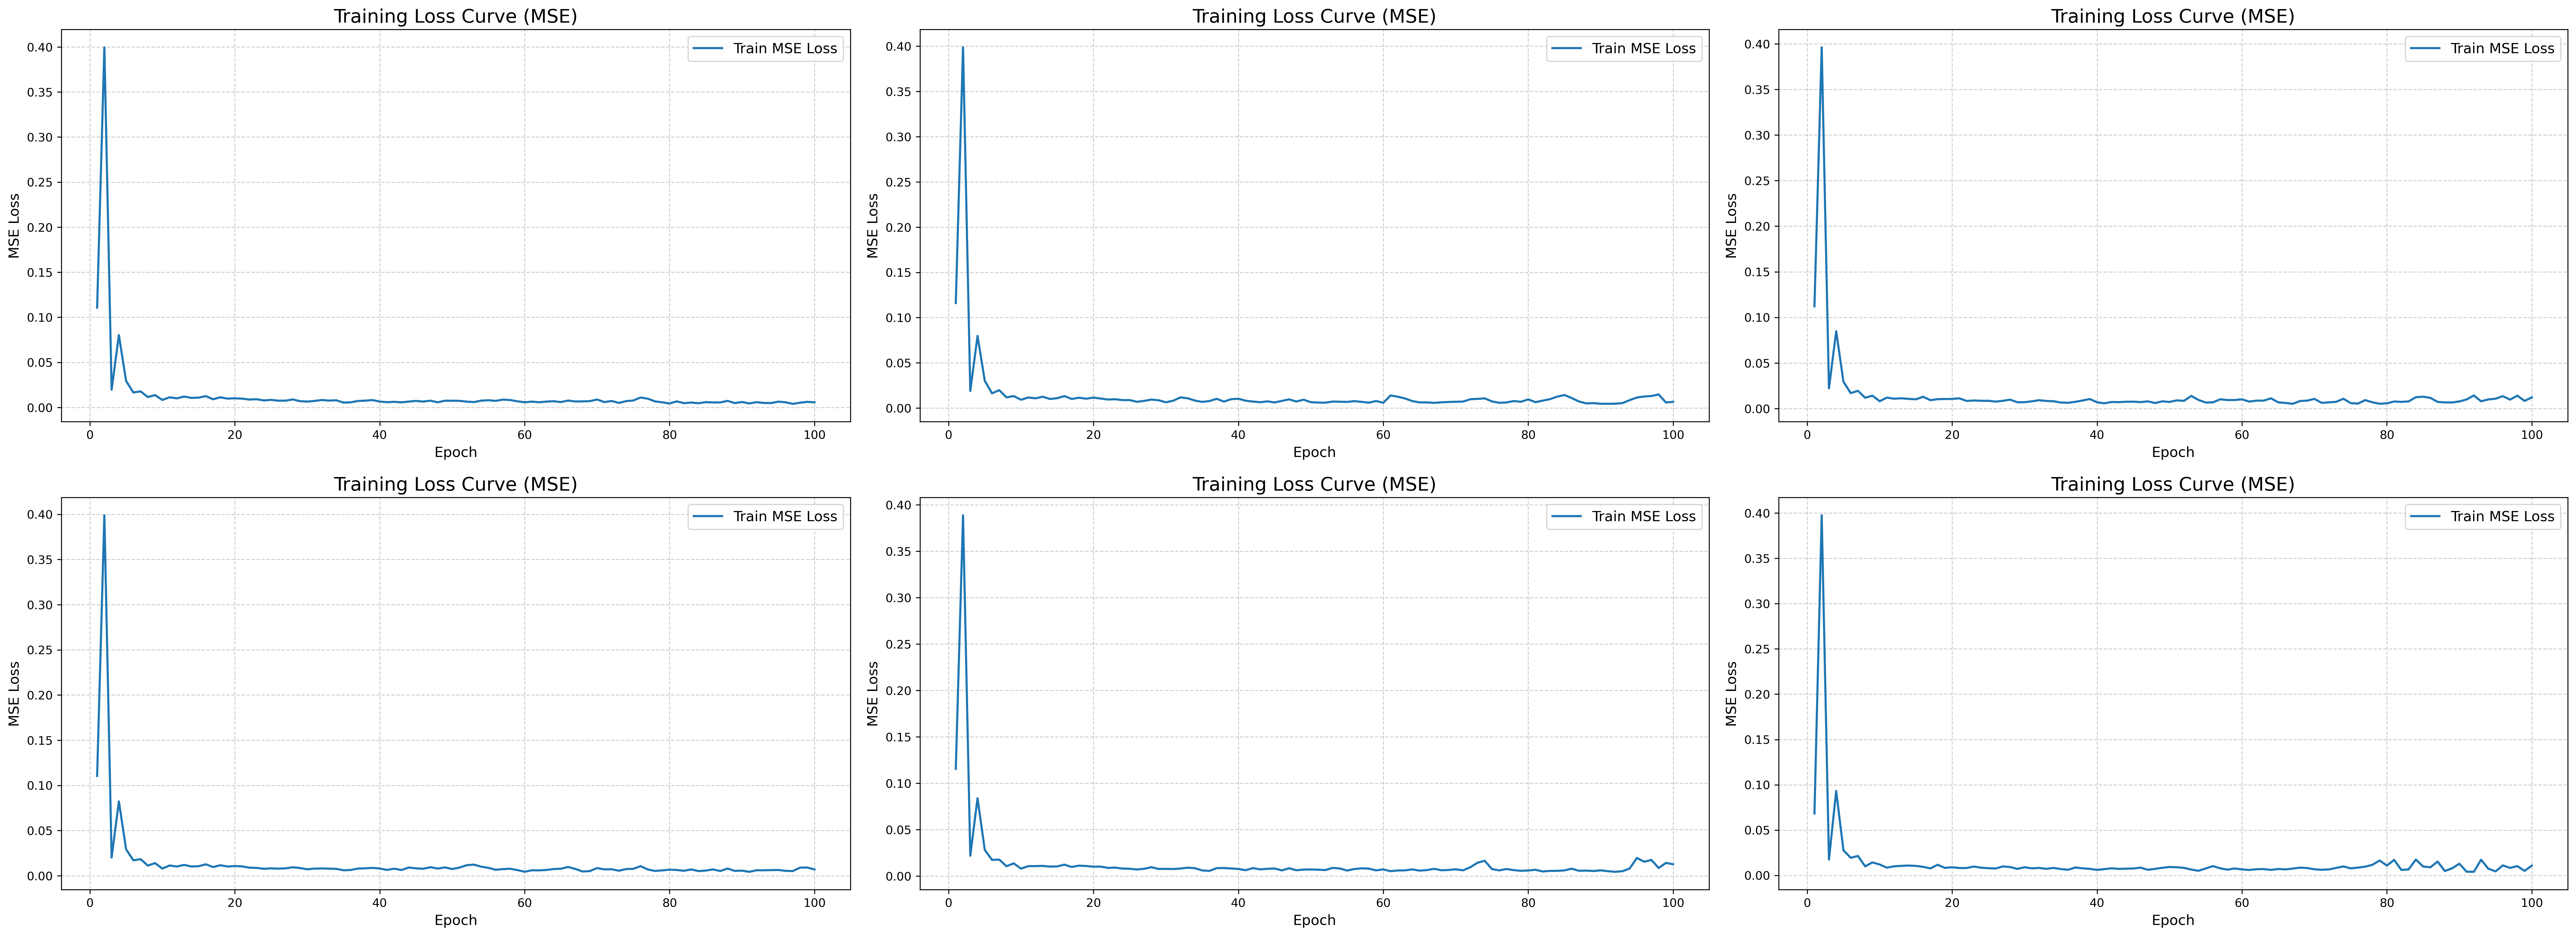
\includegraphics[width=0.8\textwidth]{figures/chap3/combined_MAA_mse_loss_curve.png} 
    \caption{GCA框架的均方误差训练损失图} % 图片下方的标题
    \label{MGCA框架的MSE训练损失图} % 【关键】设置引用标签，必须放在 \caption 之后！
\end{figure}

\begin{figure}[htbp] % [htbp] 是位置参数：这里(h)、页首(t)、页尾(b)、单独一页(p)
    \centering % 图片居中
    % width=\textwidth 表示图片宽度占满正文文本宽度
    % 如果在文件夹里，路径要是 figures/my_chart.png
    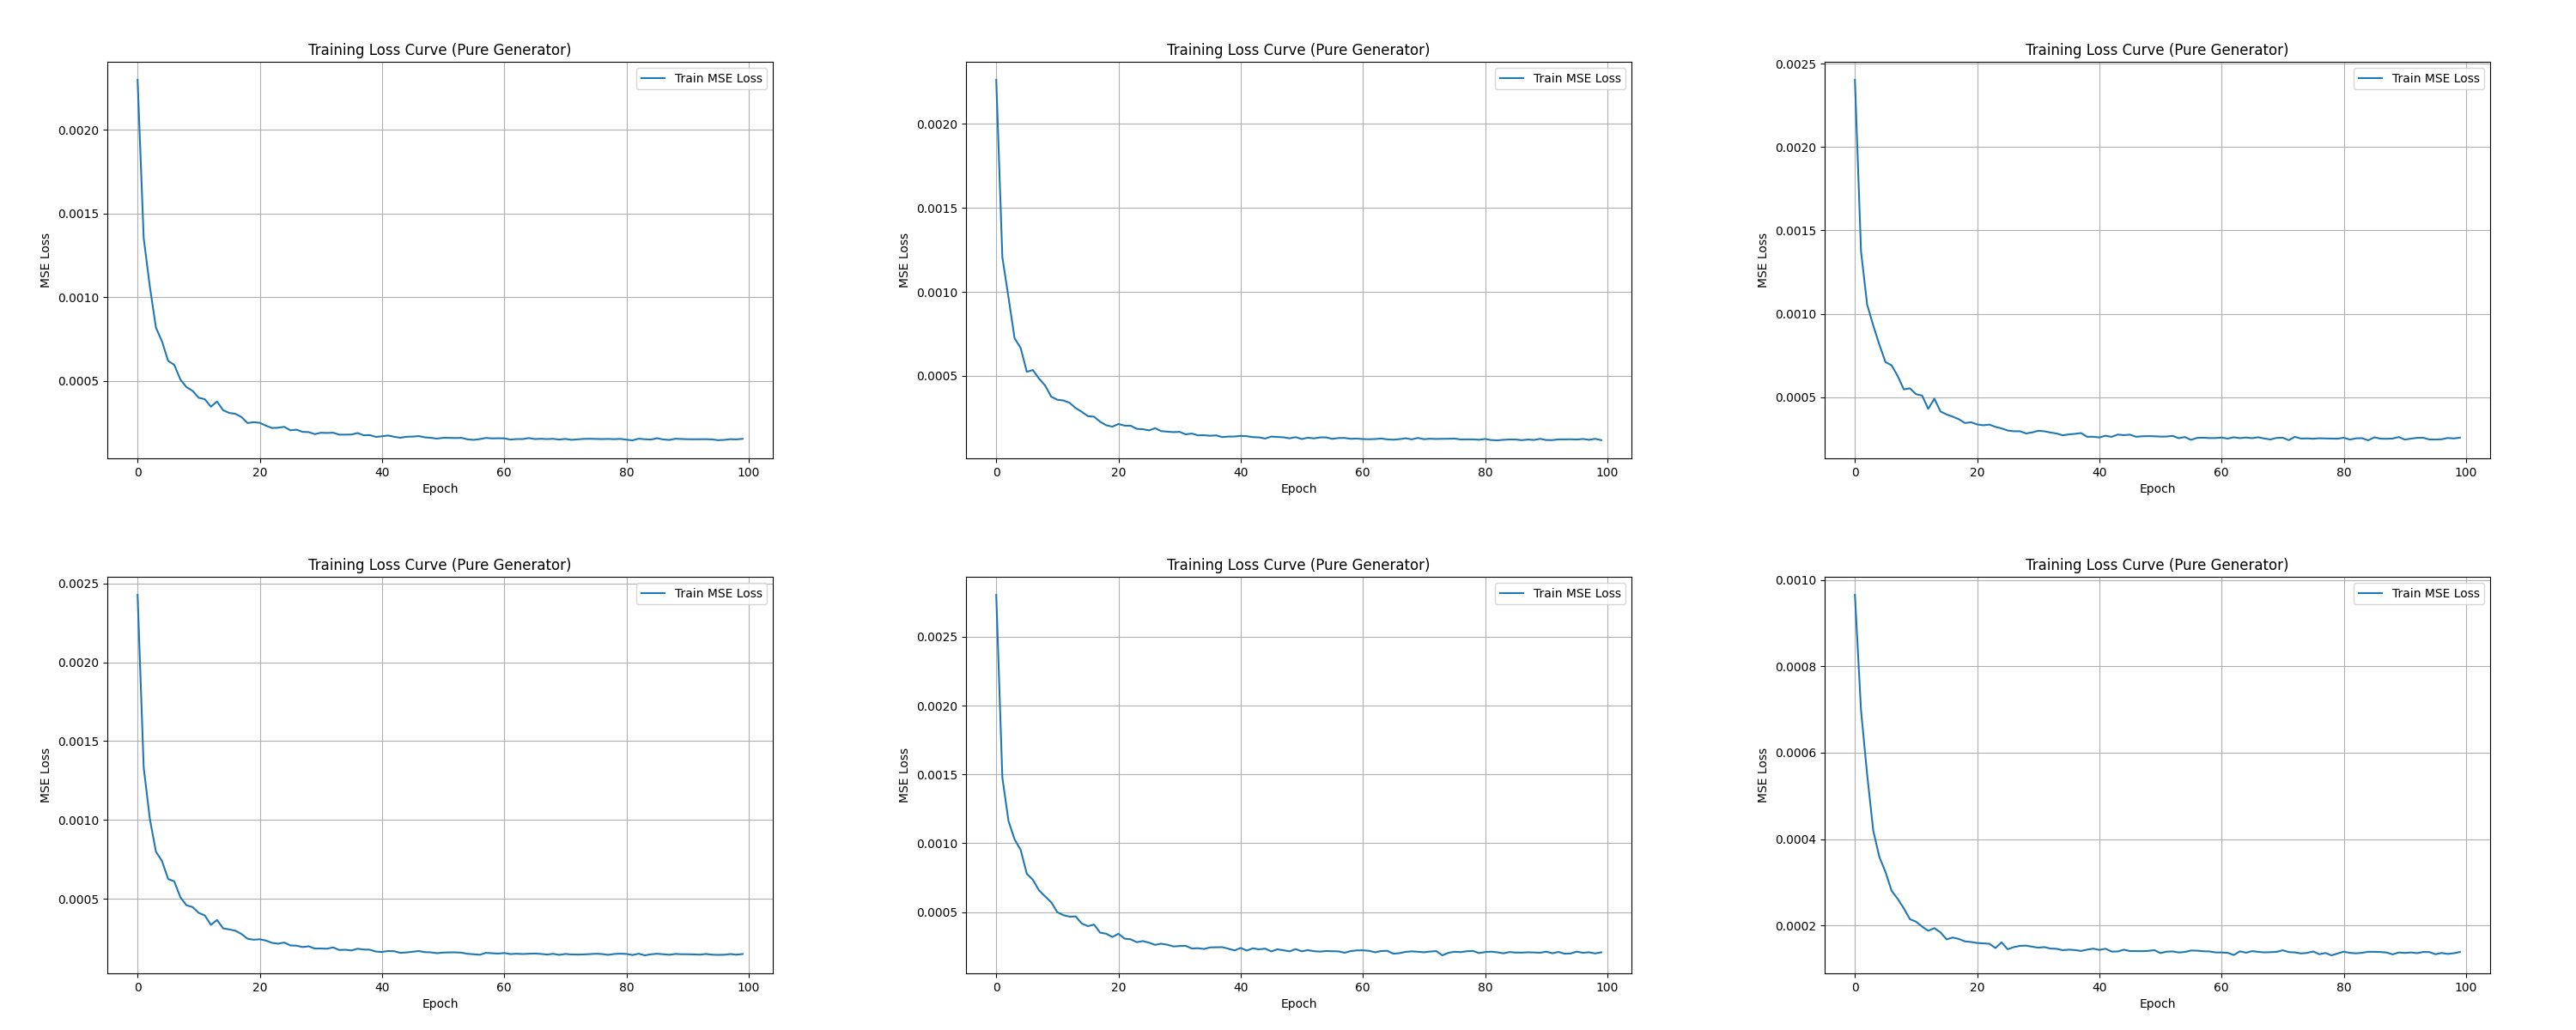
\includegraphics[width=0.8\textwidth]{figures/chap3/combined_GRU_mse_loss_curve.png} 
    \caption{门控循环单元的均方误差训练损失图} % 图片下方的标题
    \label{GRU的MSE训练损失图} % 【关键】设置引用标签，必须放在 \caption 之后！
\end{figure}

\begin{figure}[htbp] % [htbp] 是位置参数：这里(h)、页首(t)、页尾(b)、单独一页(p)
    \centering % 图片居中
    % width=\textwidth 表示图片宽度占满正文文本宽度
    % 如果在文件夹里，路径要是 figures/my_chart.png
    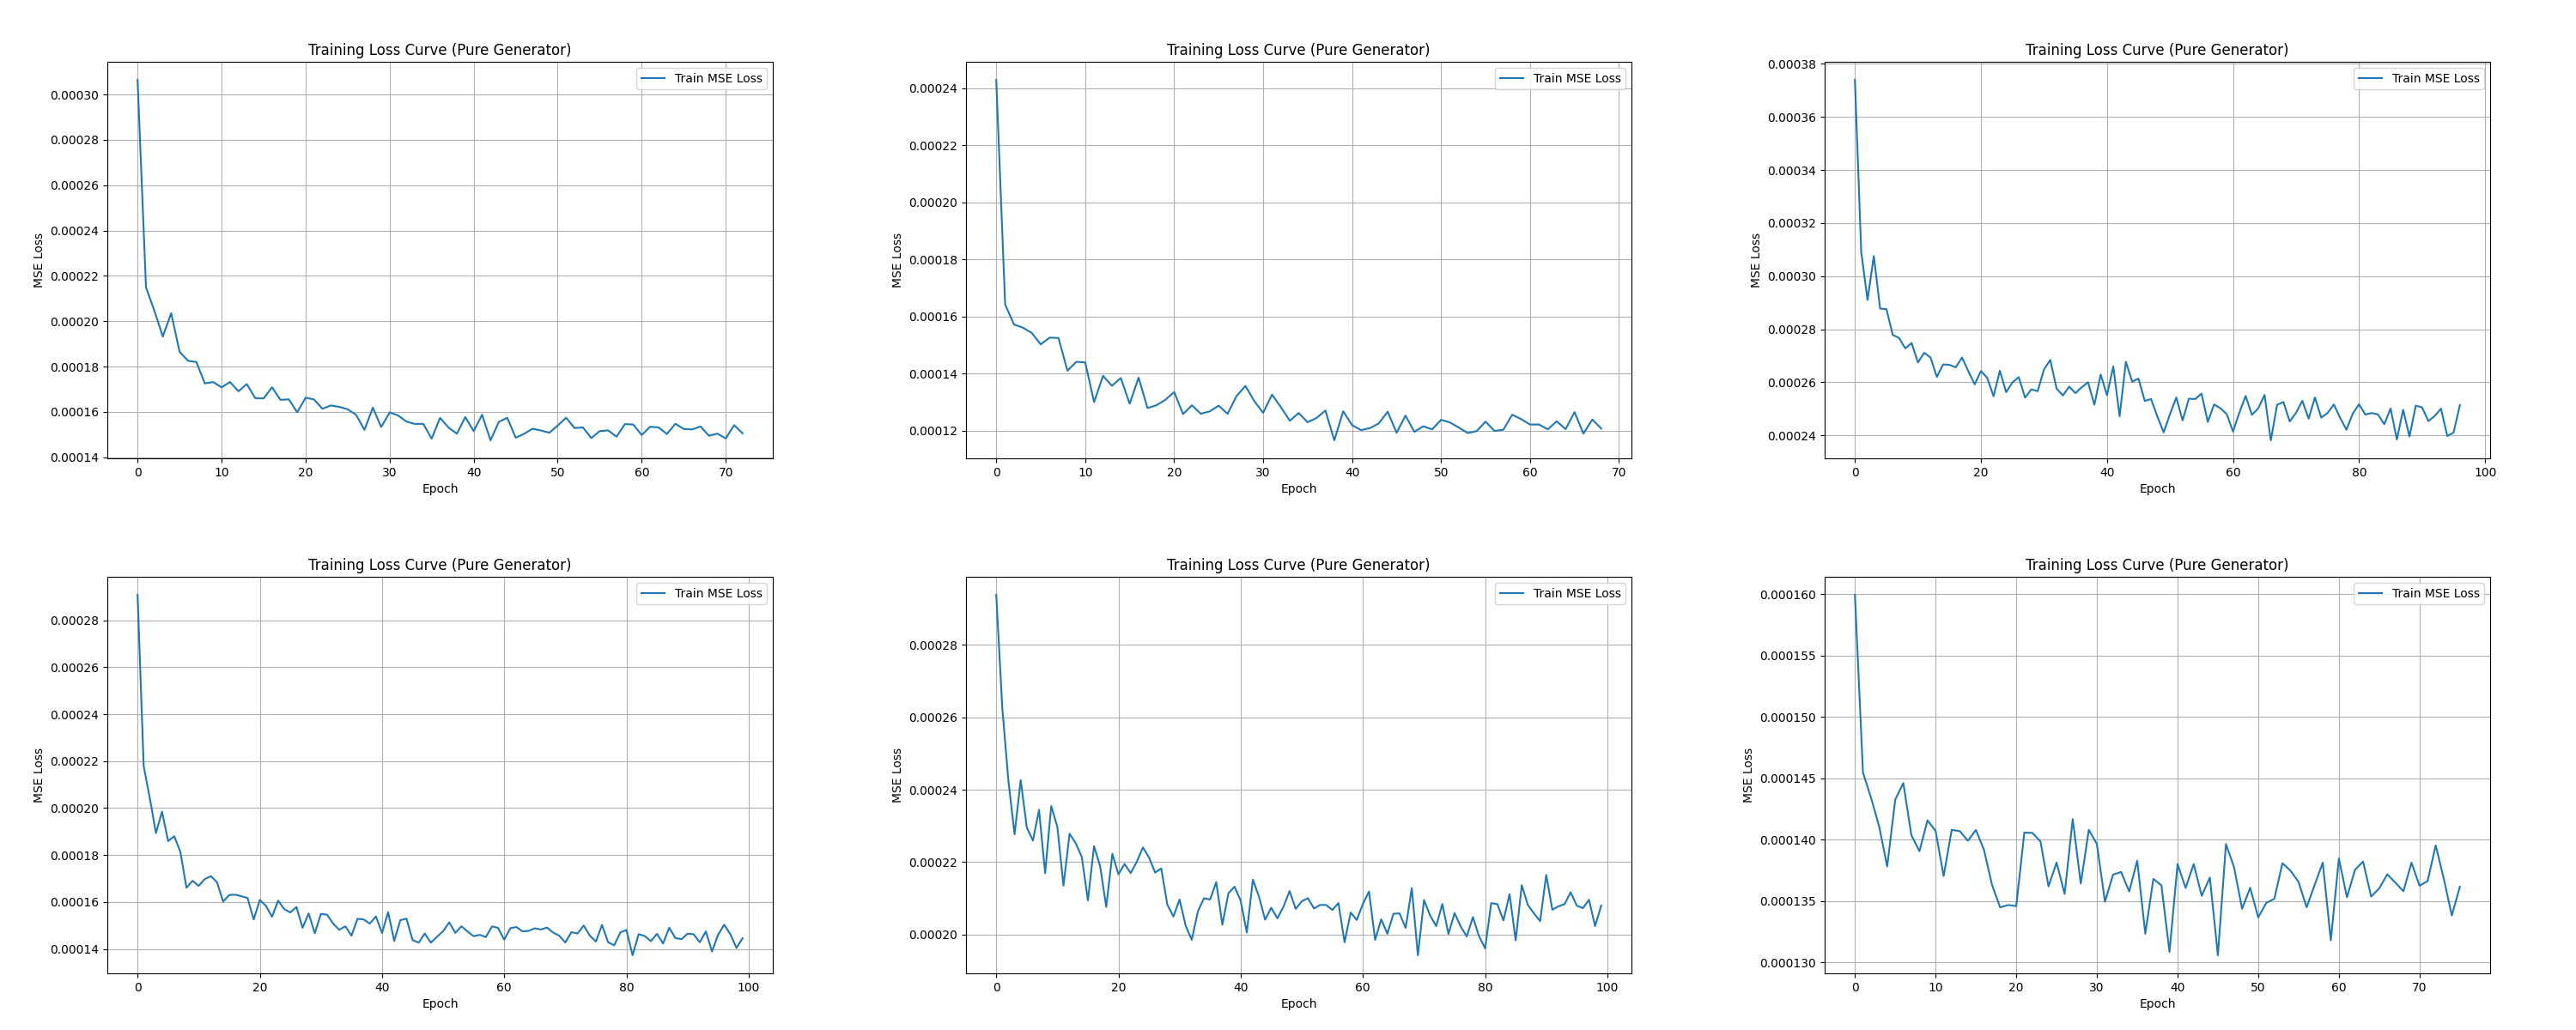
\includegraphics[width=0.8\textwidth]{figures/chap3/combined_LSTM_mse_loss_curve.png} 
    \caption{长短期记忆网络的均方误差训练损失图} % 图片下方的标题
    \label{LSTM的MSE训练损失图} % 【关键】设置引用标签，必须放在 \caption 之后！
\end{figure}

\begin{figure}[htbp] % [htbp] 是位置参数：这里(h)、页首(t)、页尾(b)、单独一页(p)
    \centering % 图片居中
    % width=\textwidth 表示图片宽度占满正文文本宽度
    % 如果在文件夹里，路径要是 figures/my_chart.png
    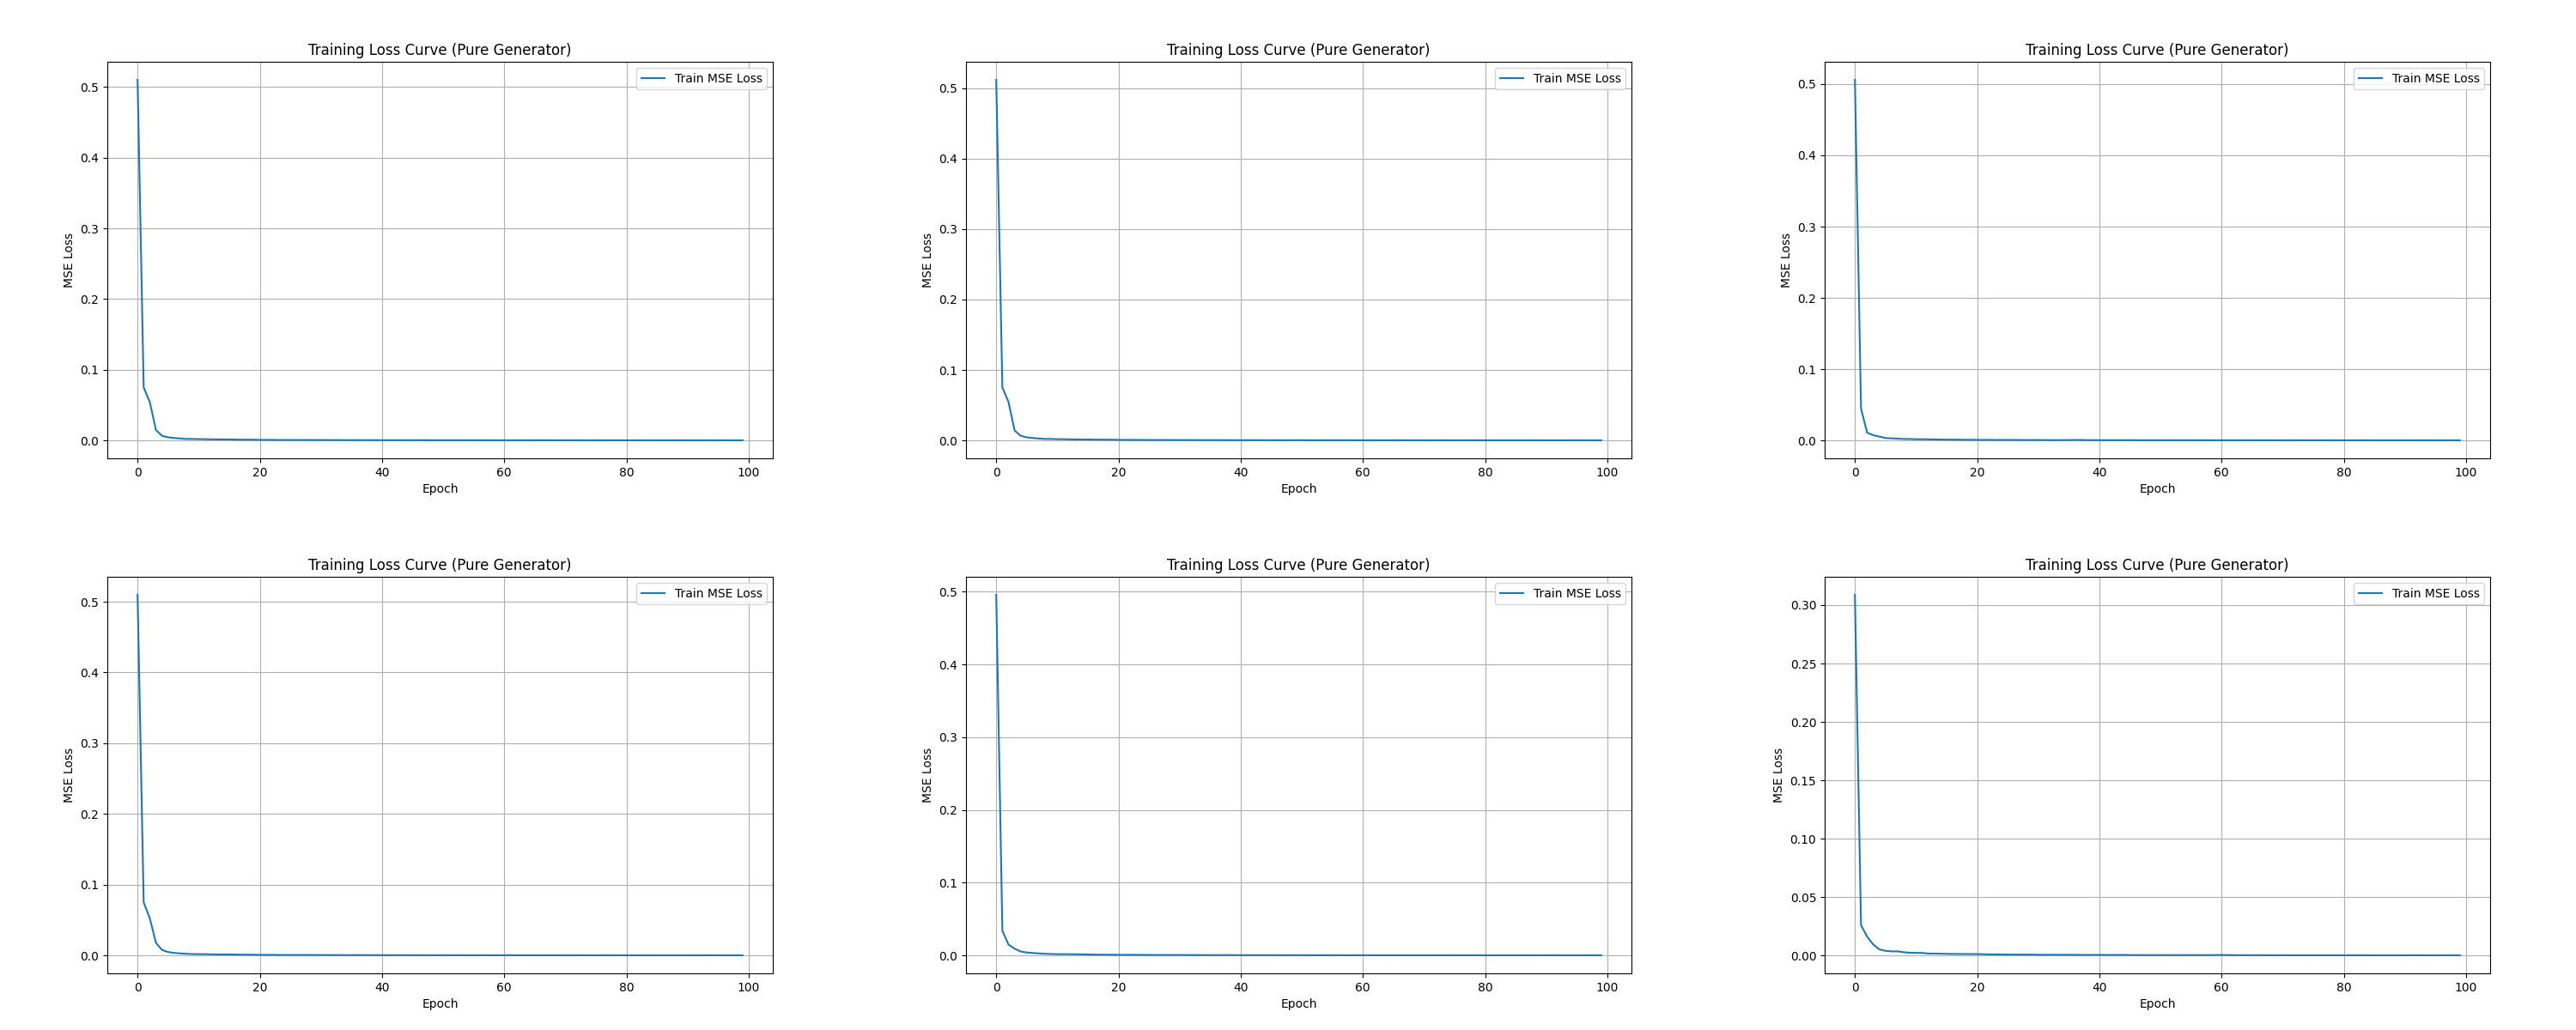
\includegraphics[width=0.8\textwidth]{figures/chap3/combined_Transformer_mse_loss_curve.png} 
    \caption{自注意力序列模型的均方误差训练损失图} % 图片下方的标题
    \label{Transformer的MSE训练损失图} % 【关键】设置引用标签，必须放在 \caption 之后！
\end{figure}

从图中可观察到明显的优化异构性：
循环神经网络（门控循环单元/长短期记忆网络）表现出早熟收敛，损失在前 10 个 Epoch 快速下降后迅速进入平台期，易过度依赖自回归特征并陷入局部最优，导致样本外对市场风格切换的适应能力较弱。
而基于对抗与注意力机制的模型（自注意力序列模型/GCA）则呈现渐进式探索，其中 GCA 损失下降平缓、微调阶段更长，有效抑制了过拟合，使模型在保证信号保真度的同时持续优化数据分布。

% \begin{enumerate}
%     \item 循环神经网络 (GRU/LSTM)：呈现出 “早熟收敛 (Premature Convergence)” 的特征。如图中第一、二列所示，RNN 类模型的损失在前 10 个 Epoch 内呈断崖式下跌，随后迅速进入平台期。这种极快的收敛往往暗示模型过度利用了时间序列的自回归特性，容易陷入局部极小值，这也解释了其在样本外测试中对市场风格转换的适应性较差。
%     \item 对抗与注意力机制 (Transformer/MGCA)：呈现出 “渐进式探索”的特征。MGCA 的损失曲线下滑斜率相对平缓，且在达到稳态前经历了更长时间的微调（Fine-tuning）。这表明MGCA有效地阻止了生成器对历史数据的过拟合，迫使其在保持信号物理保真度的同时，不断调整分布以通过判别器的统计检验。
% \end{enumerate}

尽管收敛路径各异，GCA 在六个组合上最终均收敛至与基准相当甚至更低的Loss水平（$10^{-4}$ 量级），表明该多目标优化系统有效实现了帕累托最优，未出现模式崩塌或梯度消失问题。


% \subsubsection{投资组合实证表现及分析}

表 \ref{tab:comparison_summary_full} 汇总了各模型在六个测试组合上的核心回测指标。实验结果显示，GCA 框架在多数场景下取得了较好的风险调整后收益（Sharpe Ratio）。
% \subsubsection{主要发现与归因分析}
基于表 \ref{tab:comparison_summary_full} 的结果，GCA在六类组合中总体呈现更稳定的风险调整后收益。其优势主要体现在三个方面：一是在P2、P3等趋势较清晰组合中能够保留进攻性；二是在P5高波动组合中降低基准模型失效风险；三是在P1、P4、P6等结构较复杂组合中保持较低换手率和较好的风险收益平衡。这些结果说明，GCA的核心贡献在于提升多资产投资组合管理中的信号稳定性、权重配置合理性与风险调整收益，而不是单纯依赖某一组合的收益表现。


% \begin{enumerate}[label=\arabic*.]
% \item \textbf{维度一：不同市场趋势的适应性}

% 这一维度验证模型是否仅在某些特定行情（如单边牛市）下有效，还是在各种市场环境下都能保持稳健。
% 牛市/高收益环境下的进攻能力：
% 在 P2（农产品） 和 P3（能源化工） 这种呈现明显上涨趋势的组合中，MGCA 取得了最高的累计收益率（分别为 110.50\% 和 39.42\%）。这说明在市场趋势明确时，MGCA 能够充分捕捉上涨红利，优于 Transformer 等基准模型。
% 震荡/复杂环境下的稳健性：
% 在 P1（宏观敏感） 和 P6（多元分散） 这种资产相关性复杂、宏观因子交织的场景下，MGCA 依然取得了最优的夏普比率（Sharpe Ratio）。这表明 MGCA 能够有效处理多维度的宏观噪音，提取有效信号。

% \item  \textbf{维度二：极端风险与高波动环境的防御性}

% 这是 多智能体群组交叉对抗框架表现最突出的维度，验证了其在应对市场剧烈波动或崩盘时的生存能力。
% 高波动与危机规避能力：
% P5（高波动） 是最关键的验证场景。在该组合中，基准模型（如 GRU）出现了严重的亏损（累计收益率 -68.18\%，夏普比率负值），而 MGCA 不仅实现了正向收益（47.27\%），还将最大回撤控制在 -20.83\%（远优于 GRU 的 -72.78\%）。
% 这证明了 多智能体群组交叉对抗框架具有极强的尾部风险感知能力，能够在市场极度不稳定时及时止损或切换防御策略，这是其相对于传统深度学习模型（LSTM/GRU）的核心优势。

% \item  \textbf{维度三：跨资产类别的泛化能力}

% 这一维度验证模型是否“过拟合”于某一类特定资产（如只懂股票不懂期货），还是在不同属性的资产上都能通用。
% 资产属性的广泛覆盖：
% 表格涵盖了大宗商品（P2 农产品、P3 能源）、金融属性强的资产（P4 避险对冲，通常包含黄金/国债等）以及混合资产（P6）。
% MGCA 在所有这些截然不同的资产类别中，夏普比率均稳定在 0.4 到 0.7 之间，且 consistently（一致地）优于其他模型。
% 低换手率带来的交易优势：
% 观察“平均换手”一列，MGCA 在绝大多数组合（P1, P2, P3, P4, P5）中的换手率都是最低的。这意味着 MGCA 不仅能适应不同资产，还能生成更平滑、噪音更少的交易信号，减少了不必要的摩擦成本，体现了其对资产底层逻辑的深刻理解而非简单的过拟合。
% \end{enumerate}


\begin{table}[H]
\centering
\caption{GCA 与基准模型在全部六个实验组合上的完整回测表现对比}
\label{tab:comparison_summary_full}
\footnotesize
\setlength{\tabcolsep}{1.5pt}
\renewcommand{\arraystretch}{1.15}
\begin{tabular}{@{}p{0.115\textwidth}p{0.145\textwidth}p{0.085\textwidth}p{0.085\textwidth}p{0.095\textwidth}p{0.095\textwidth}p{0.095\textwidth}p{0.070\textwidth}p{0.075\textwidth}@{}}
\toprule
\textbf{组合} & \textbf{模型} & \textbf{夏普比率} & \textbf{卡玛比率} & \textbf{累计收益率} & \textbf{年化波动率} & \textbf{最大回撤} & \textbf{胜率} & \textbf{平均换手} \\
\midrule
\multirow{4}{*}{\shortstack[l]{P1 宏观敏感}}
& 门控循环单元 & 0.279 & 0.143 & 17.86\% & 12.97\% & -25.36\% & 50.4\% & 0.050 \\
& 长短期记忆网络 & 0.225 & 0.122 & 14.03\% & 12.63\% & -23.41\% & 50.6\% & 0.038 \\
& 自注意力序列模型 & 0.384 & 0.286 & 24.67\% & 12.99\% & -17.51\% & 50.1\% & 0.055 \\
& \textbf{GCA} & \textbf{0.421} & \textbf{0.269} & \textbf{26.93\%} & 13.18\% & \textbf{-20.59\%} & \textbf{51.1\%} & \textbf{0.024} \\
\midrule
\multirow{4}{*}{\shortstack[l]{P2 农产品}}
& 门控循环单元 & 0.430 & 0.235 & 73.12\% & 10.16\% & -18.60\% & 50.1\% & 0.092 \\
& 长短期记忆网络 & 0.603 & 0.335 & 101.93\% & 10.09\% & -18.22\% & 50.3\% & 0.055 \\
& 自注意力序列模型 & 0.604 & 0.363 & 102.31\% & 10.11\% & -16.86\% & 50.6\% & 0.040 \\
& \textbf{GCA} & \textbf{0.657} & \textbf{0.402} & \textbf{110.50\%} & 10.10\% & \textbf{-16.50\%} & \textbf{50.9\%} & \textbf{0.039} \\
\midrule
\multirow{4}{*}{\shortstack[l]{P3 能源化工}}
& 门控循环单元 & 0.313 & 0.254 & 21.51\% & 13.93\% & -17.14\% & 49.1\% & 0.090 \\
& 长短期记忆网络 & 0.354 & 0.277 & 24.69\% & 14.15\% & -18.08\% & 48.7\% & 0.075 \\
& 自注意力序列模型 & 0.515 & 0.480 & 35.87\% & 14.13\% & -15.14\% & 49.2\% & 0.077 \\
& \textbf{GCA} & \textbf{0.581} & \textbf{0.609} & \textbf{39.42\%} & 13.99\% & \textbf{-13.35\%} & \textbf{49.7\%} & \textbf{0.033} \\
\bottomrule
\end{tabular}
\end{table}
\begin{table}[H]
\centering
{\small\textbf{续表}}\\[0.5em]
\footnotesize
\setlength{\tabcolsep}{1.5pt}
\renewcommand{\arraystretch}{1.15}
\begin{tabular}{@{}p{0.115\textwidth}p{0.145\textwidth}p{0.085\textwidth}p{0.085\textwidth}p{0.095\textwidth}p{0.095\textwidth}p{0.095\textwidth}p{0.070\textwidth}p{0.075\textwidth}@{}}
\toprule
\textbf{组合} & \textbf{模型} & \textbf{夏普比率} & \textbf{卡玛比率} & \textbf{累计收益率} & \textbf{年化波动率} & \textbf{最大回撤} & \textbf{胜率} & \textbf{平均换手} \\
\midrule
\multirow{4}{*}{\shortstack[l]{P4 避险对冲}}
& 门控循环单元 & 0.564 & 0.455 & 34.41\% & 22.46\% & -27.84\% & 48.8\% & 0.085 \\
& 长短期记忆网络 & 0.616 & 0.528 & 37.10\% & 22.18\% & -25.88\% & 48.9\% & 0.070 \\
& 自注意力序列模型 & 0.657 & 0.546 & 37.72\% & 21.17\% & -25.47\% & 48.5\% & 0.058 \\
& \textbf{GCA} & \textbf{0.692} & \textbf{0.628} & \textbf{39.48\%} & 21.65\% & \textbf{-23.85\%} & 48.2\% & \textbf{0.038} \\
\midrule
\multirow{4}{*}{\shortstack[l]{P5 高波动}}
& 门控循环单元 & -0.750 & -0.105 & -68.18\% & 10.23\% & -72.78\% & 47.4\% & 0.373 \\
& 长短期记忆网络 & 0.118 & 0.049 & 10.58\% & 10.05\% & -24.33\% & 49.4\% & 0.124 \\
& 自注意力序列模型 & 0.067 & 0.024 & 5.88\% & 9.85\% & -27.29\% & 49.5\% & 0.122 \\
& \textbf{GCA} & \textbf{0.543} & \textbf{0.258} & \textbf{47.27\%} & 9.88\% & \textbf{-20.83\%} & \textbf{51.1\%} & \textbf{0.035} \\
\midrule
\multirow{4}{*}{\shortstack[l]{P6 多元分散}}
& 门控循环单元 & 0.471 & 0.380 & 44.81\% & 13.56\% & -16.79\% & 51.9\% & 0.070 \\
& 长短期记忆网络 & 0.365 & 0.268 & 32.62\% & 12.74\% & -17.33\% & 51.6\% & 0.082 \\
& 自注意力序列模型 & 0.436 & 0.398 & 41.87\% & 13.67\% & -14.98\% & 52.0\% & 0.048 \\
& \textbf{GCA} & \textbf{0.562} & \textbf{0.571} & \textbf{52.84\%} & 13.55\% & \textbf{-13.34\%} & 51.6\% & 0.070 \\
\bottomrule
\end{tabular}
\end{table}


% \subsubsection{产业链传导与宏观对冲能力的验证}

从组合差异看，P3的能源化工组合验证了GCA对产业链时滞关系的捕捉能力，P4说明该架构在宏观对冲组合中能够改善盈亏结构，P5则体现了其在高波动环境下的防御性。P1和P2的结果进一步表明，GCA并非只在单一市场状态下有效，而是能够通过异构智能体的协同分工，在趋势、震荡和低相关资产池中维持较稳定的信号生成能力。

\noindent\textbf{辅助校验层的实证效果}\par

为观察辅助校验层对GCA输出权重的影响，本节在六组实验组合上比较GCA模型与接入量化相对强度指标过滤后的样本外回测表现。该实验不改变GCA主体结构，仅在模型输出后增加状态确认与权重过滤。表 \ref{tab:qr_gca_results} 汇总了对比结果。

\begin{table}[H]
\centering
\caption{GCA 与辅助校验层在六类组合上的回测对比}
\label{tab:qr_gca_results}
\footnotesize
\setlength{\tabcolsep}{2pt}
\renewcommand{\arraystretch}{1.15}
\begin{tabular}{@{}p{0.15\textwidth}p{0.18\textwidth}p{0.085\textwidth}p{0.095\textwidth}p{0.095\textwidth}p{0.095\textwidth}p{0.075\textwidth}p{0.085\textwidth}@{}}
\toprule
\textbf{组合} & \textbf{方法} & \textbf{夏普比率} & \textbf{累计收益率} & \textbf{年化收益率} & \textbf{最大回撤} & \textbf{胜率} & \textbf{$\Delta$ Sharpe} \\
\midrule
\multirow{2}{*}{\shortstack[l]{P1 宏观敏感\\(Gold,Oil,Cu,M)}}
& GCA & 0.4193 & 26.91\% & 5.54\% & -20.44\% & 50.78\% & --- \\
& \textbf{GCA+辅助校验层} & \textbf{1.6082} & \textbf{199.09\%} & \textbf{41.02\%} & -21.91\% & 52.25\% & \textbf{+1.1889} \\
\midrule
\multirow{2}{*}{\shortstack[l]{P2 农产品\\(Corn,M,SR,CF)}}
& GCA & 0.6687 & 112.49\% & 6.76\% & -16.63\% & 50.88\% & --- \\
& \textbf{GCA+辅助校验层} & \textbf{1.0208} & \textbf{193.29\%} & \textbf{11.61\%} & -16.63\% & 48.71\% & \textbf{+0.3521} \\
\bottomrule
\end{tabular}
\end{table}
\begin{table}[H]
\centering
{\small\textbf{续表}}\\[0.5em]
\footnotesize
\setlength{\tabcolsep}{2pt}
\renewcommand{\arraystretch}{1.15}
\begin{tabular}{@{}p{0.15\textwidth}p{0.18\textwidth}p{0.085\textwidth}p{0.095\textwidth}p{0.095\textwidth}p{0.095\textwidth}p{0.075\textwidth}p{0.085\textwidth}@{}}
\toprule
\textbf{组合} & \textbf{方法} & \textbf{夏普比率} & \textbf{累计收益率} & \textbf{年化收益率} & \textbf{最大回撤} & \textbf{胜率} & \textbf{$\Delta$ Sharpe} \\
\midrule
\multirow{2}{*}{\shortstack[l]{P3 能源化工\\(Oil,MA,PP,TA)}}
& GCA & 0.4936 & 42.91\% & 4.88\% & -20.08\% & 51.31\% & --- \\
& \textbf{GCA+辅助校验层} & \textbf{1.1148} & \textbf{141.43\%} & \textbf{16.07\%} & -32.17\% & 49.37\% & \textbf{+0.6212} \\
\midrule
\multirow{2}{*}{\shortstack[l]{P4 避险对冲\\(Au,Cu,Oil,ZC)}}
& GCA & 0.7077 & 40.57\% & 15.4\% & -24.25\% & 48.04\% & --- \\
& GCA+辅助校验层 & 0.4086 & 30.58\% & 11.61\% & -34.58\% & 45.63\% & -0.2991 \\
\bottomrule
\end{tabular}
\end{table}
\begin{table}[H]
\centering
{\small\textbf{续表}}\\[0.5em]
\footnotesize
\setlength{\tabcolsep}{2pt}
\renewcommand{\arraystretch}{1.15}
\begin{tabular}{@{}p{0.15\textwidth}p{0.18\textwidth}p{0.085\textwidth}p{0.095\textwidth}p{0.095\textwidth}p{0.095\textwidth}p{0.075\textwidth}p{0.085\textwidth}@{}}
\toprule
\textbf{组合} & \textbf{方法} & \textbf{夏普比率} & \textbf{累计收益率} & \textbf{年化收益率} & \textbf{最大回撤} & \textbf{胜率} & \textbf{$\Delta$ Sharpe} \\
\midrule
\multirow{2}{*}{\shortstack[l]{P5 高波动\\(V,MA,TA,PP)}}
& GCA & 0.4819 & 41.87\% & 4.76\% & -20.64\% & 51.35\% & --- \\
& \textbf{GCA+辅助校验层} & \textbf{1.1235} & \textbf{142.01\%} & \textbf{16.13\%} & -34.88\% & 49.91\% & \textbf{+0.6416} \\
\midrule
\multirow{2}{*}{\shortstack[l]{P6 多元分散\\(Au,CF,I,SR,ZC)}}
& GCA & 0.5723 & 53.16\% & 7.66\% & -12.94\% & 51.6\% & --- \\
& \textbf{GCA+辅助校验层} & \textbf{0.8214} & \textbf{111.35\%} & \textbf{16.05\%} & -14.33\% & 50.23\% & \textbf{+0.2491} \\
\bottomrule
\end{tabular}
\end{table}


\begin{figure}[htbp]
    \centering
    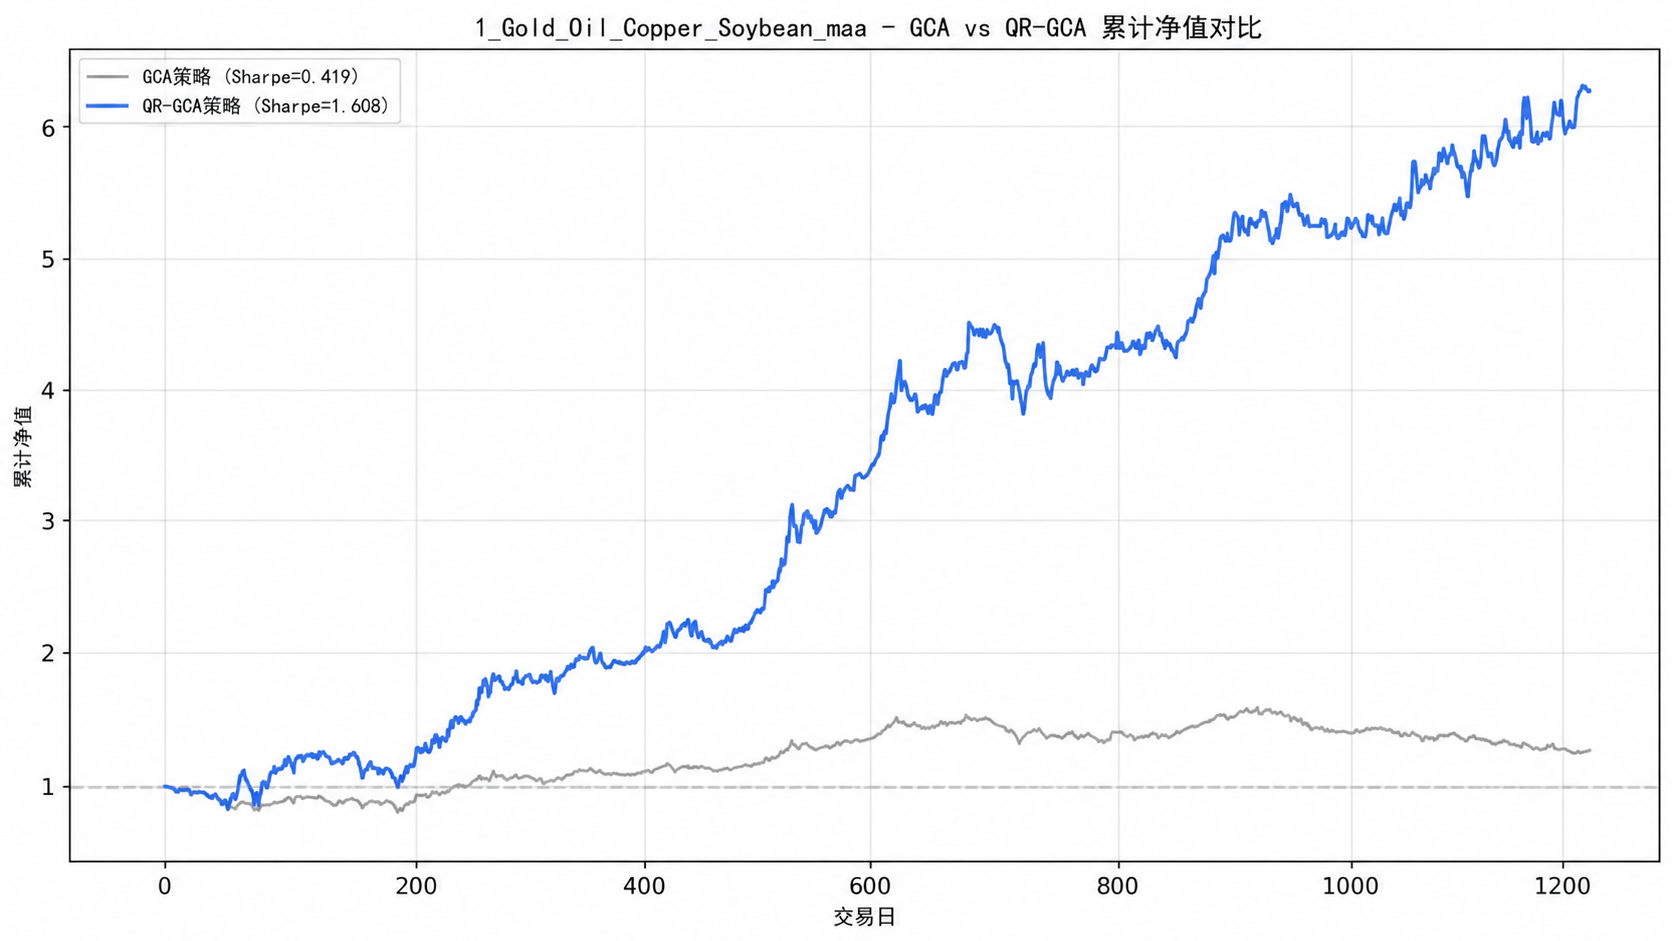
\includegraphics[width=0.48\textwidth]{figures/chap3/qr_gca/P1_comparison.png}
    \hfill
    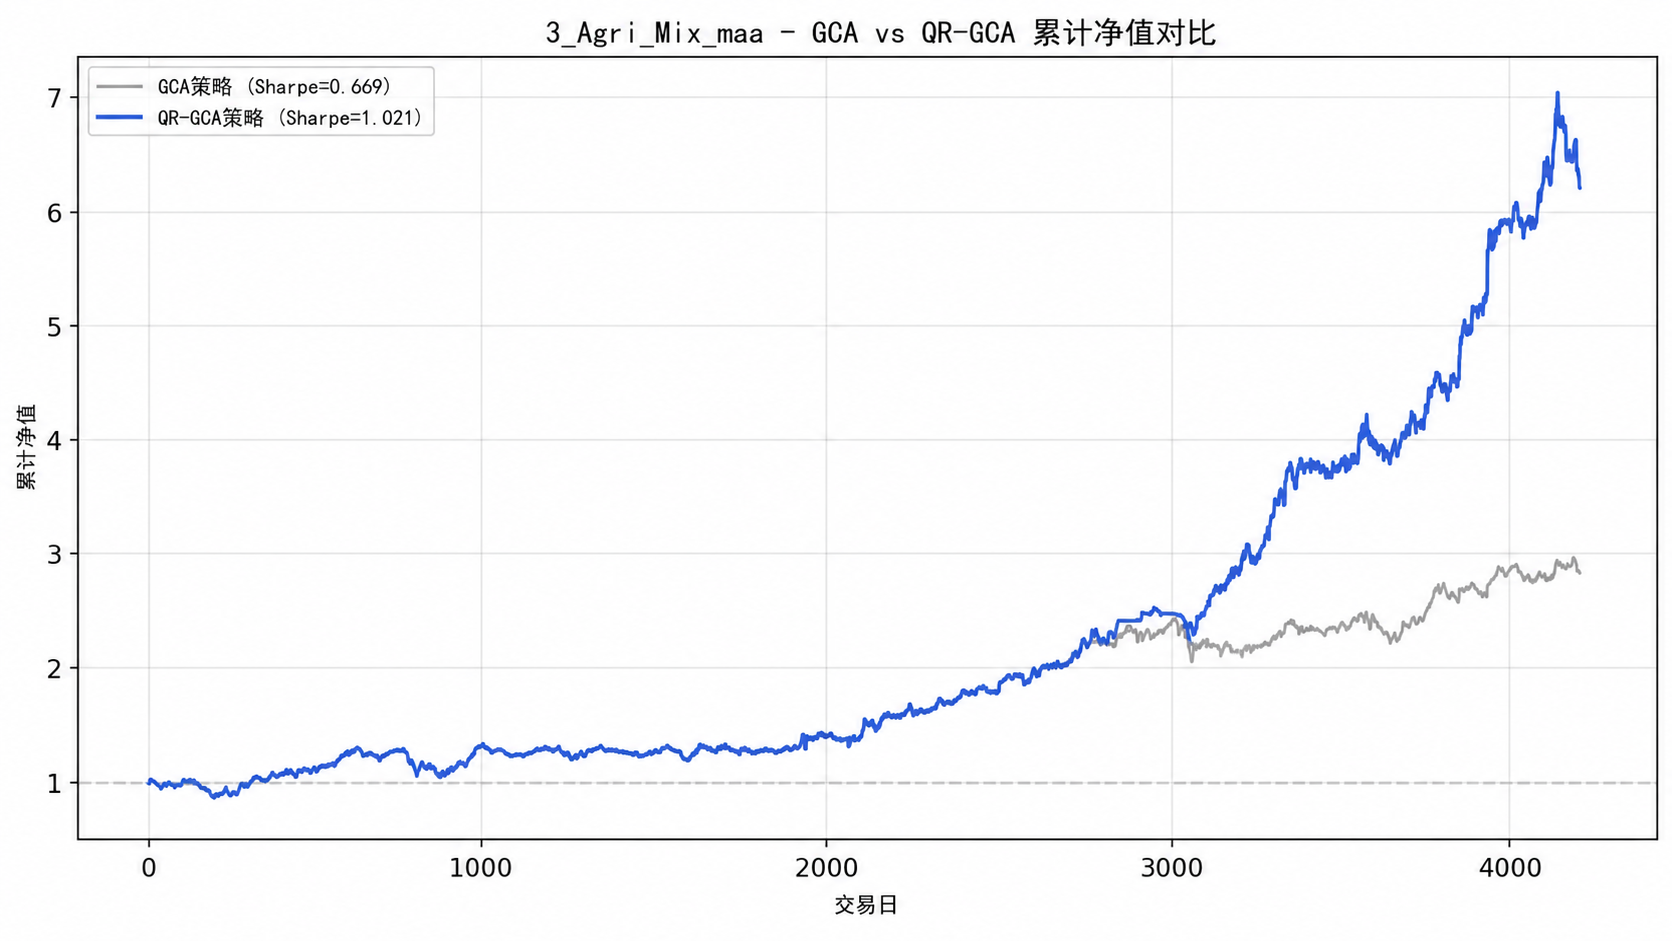
\includegraphics[width=0.48\textwidth]{figures/chap3/qr_gca/P2_comparison.png}
    \\[0.5em]
    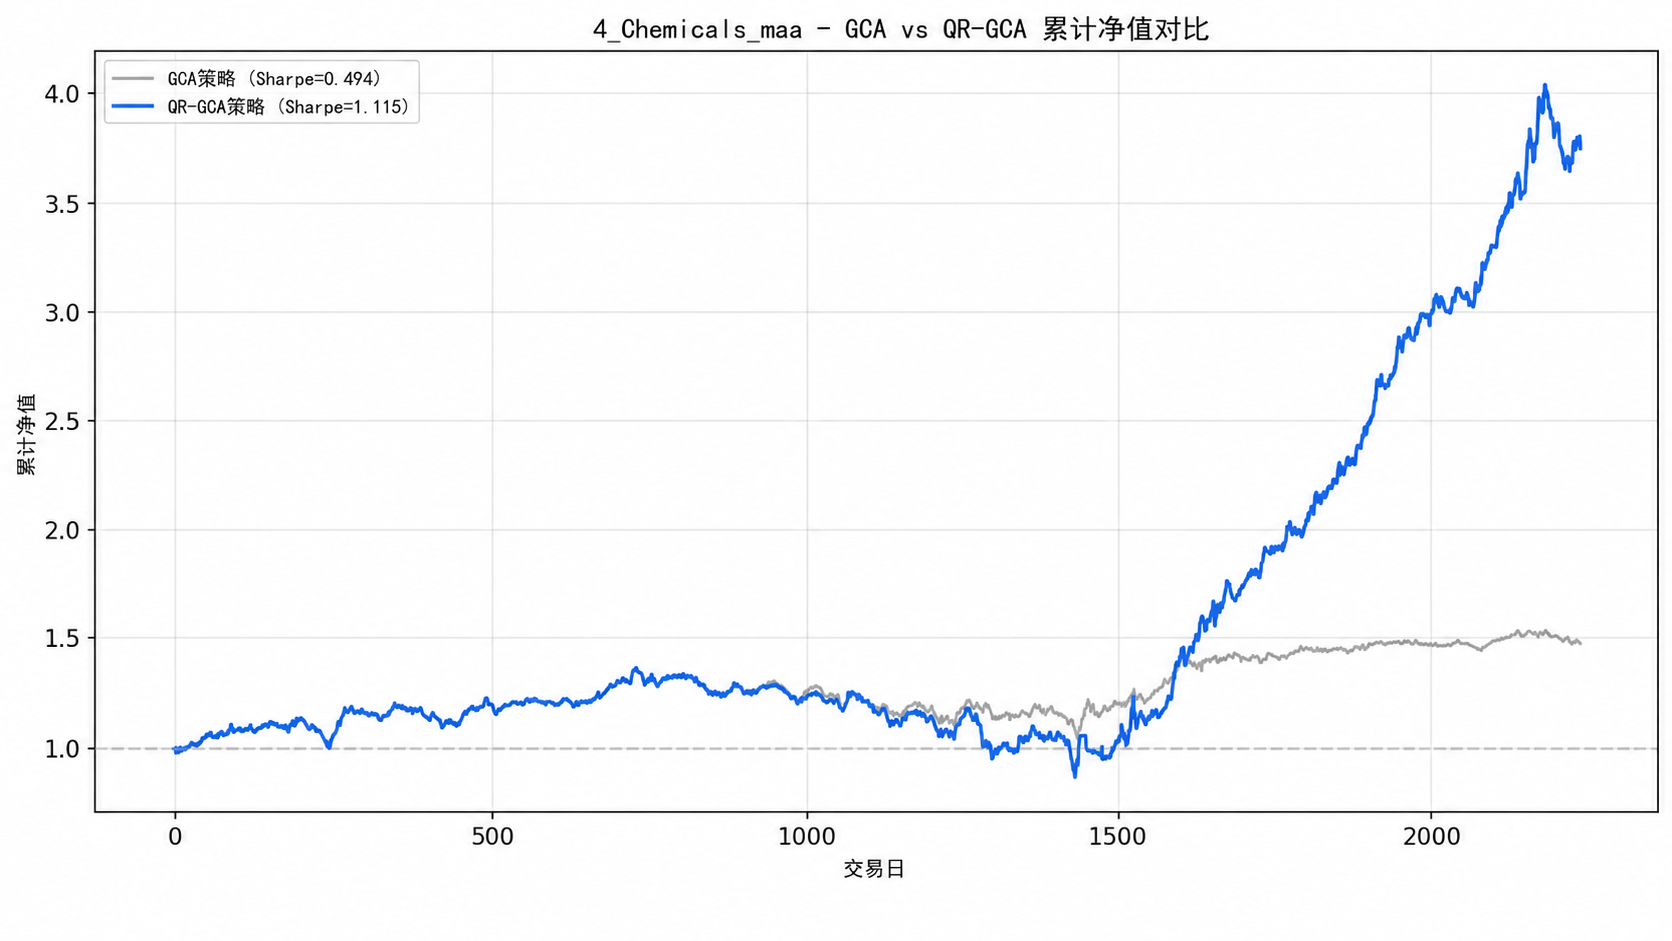
\includegraphics[width=0.48\textwidth]{figures/chap3/qr_gca/P3_comparison.png}
    \hfill
    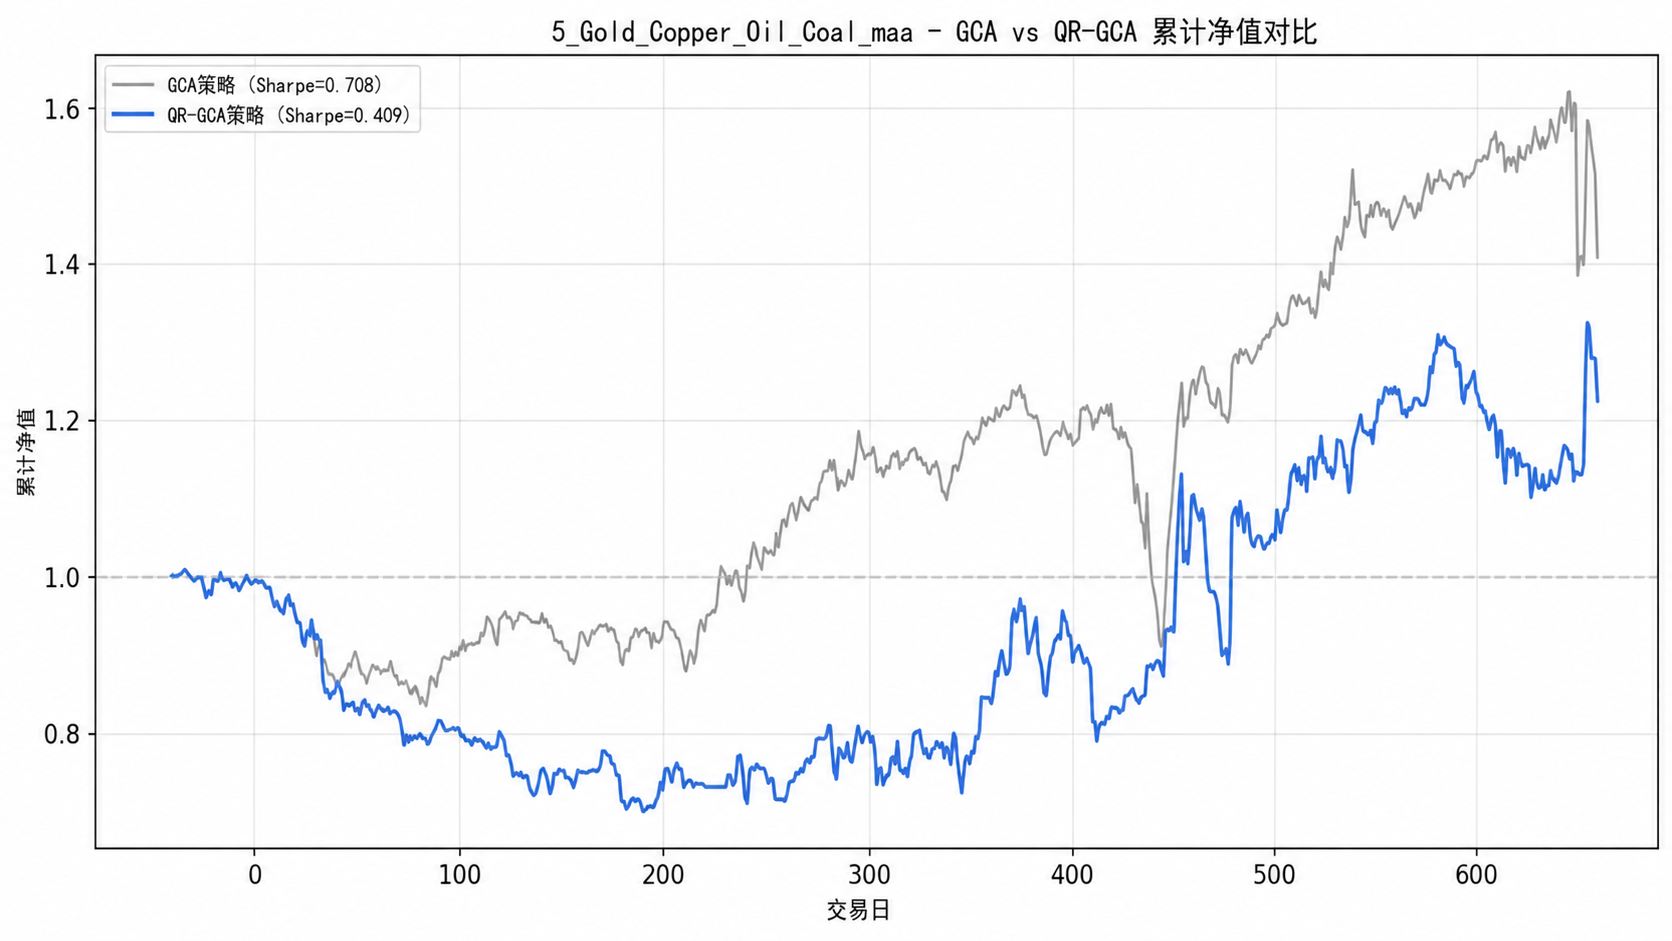
\includegraphics[width=0.48\textwidth]{figures/chap3/qr_gca/P4_comparison.png}
    \\[0.5em]
    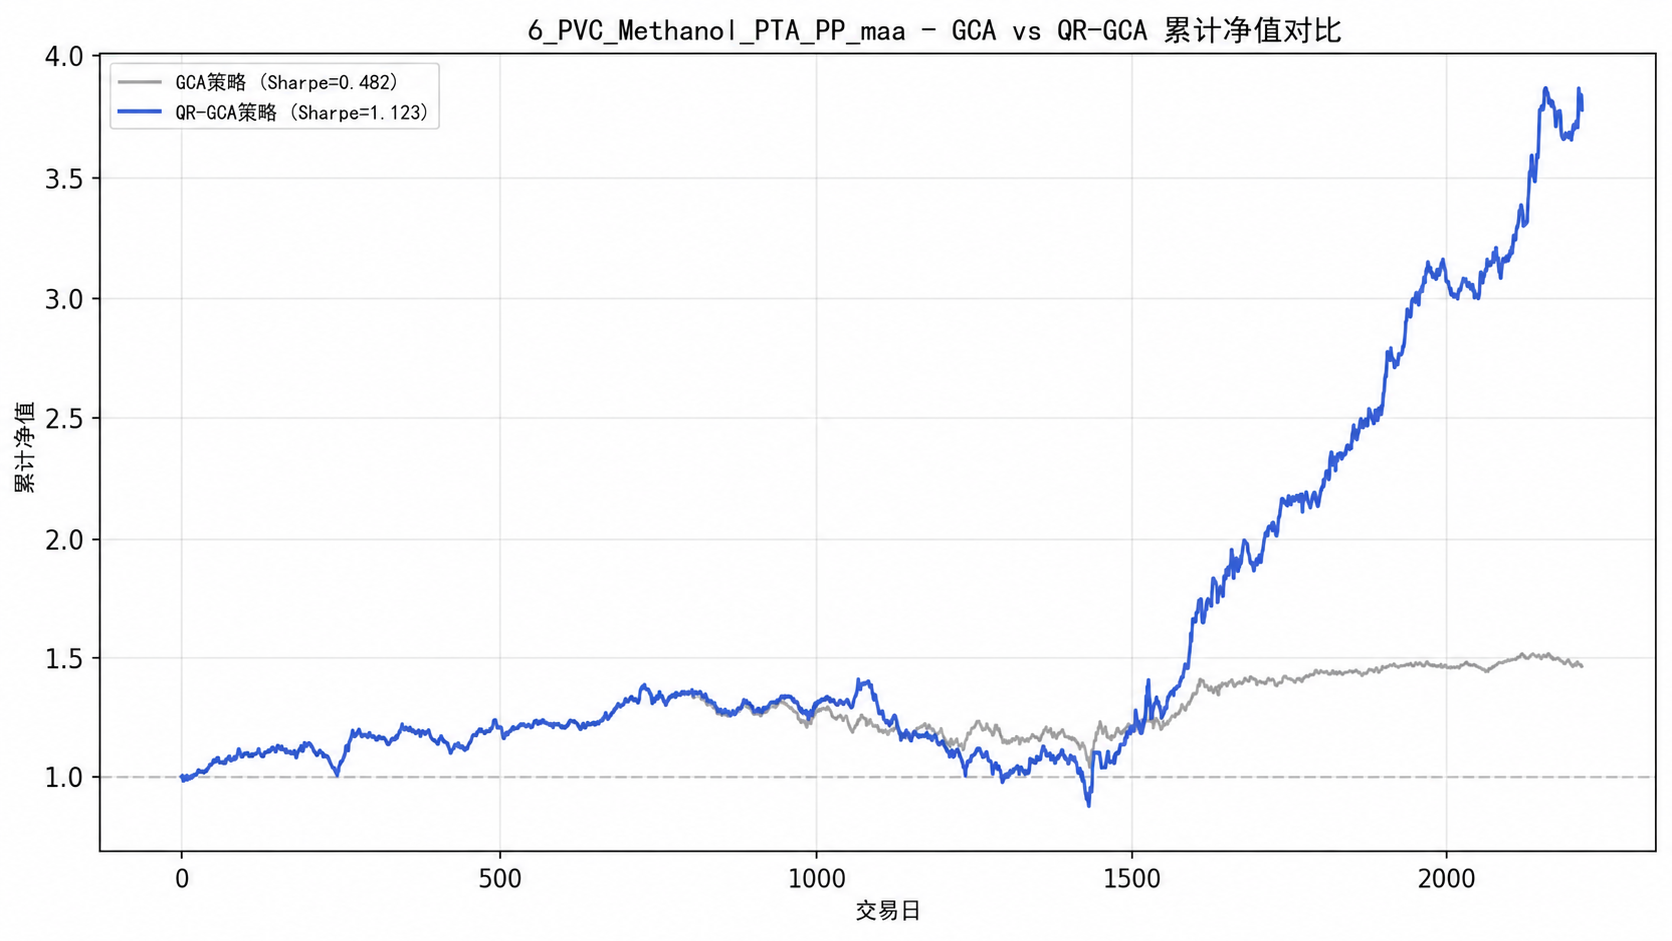
\includegraphics[width=0.48\textwidth]{figures/chap3/qr_gca/P5_comparison.png}
    \hfill
    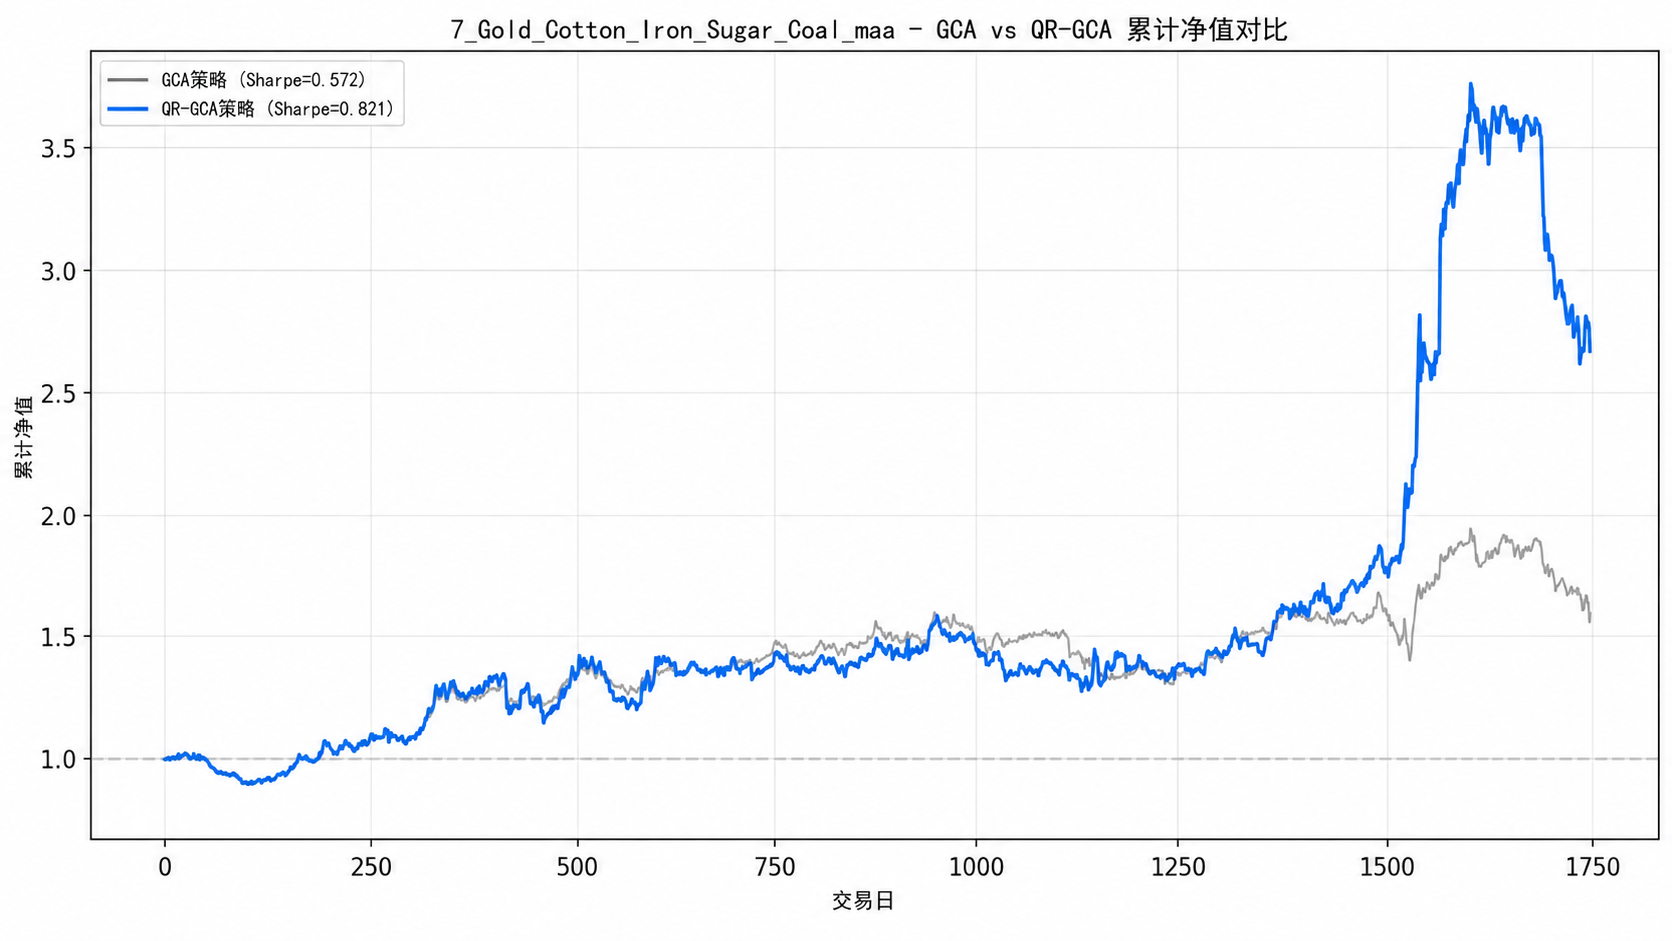
\includegraphics[width=0.48\textwidth]{figures/chap3/qr_gca/P6_comparison.png}
    \caption{GCA 与辅助校验层累计净值对比}
    \label{fig:qr_gca_comparison}
\end{figure}

% \subsubsection{辅助校验的系统性提升分析}

表 \ref{tab:qr_gca_results} 与图 \ref{fig:qr_gca_comparison} 显示，辅助校验层在多数趋势性组合中改善了GCA输出的交易可用性。P1、P2、P3、P5和P6的夏普比率均有提升，说明相对强弱确认在趋势性较强的组合中具有一定过滤价值。P4表现下降则表明，当组合收益主要来自跨资产对冲而非单向趋势时，统一市场状态过滤可能压制有效仓位。因此，该模块应被理解为GCA输出后的校验层，而不是本章的主要方法贡献。

\begin{figure}[htbp]
    \centering
    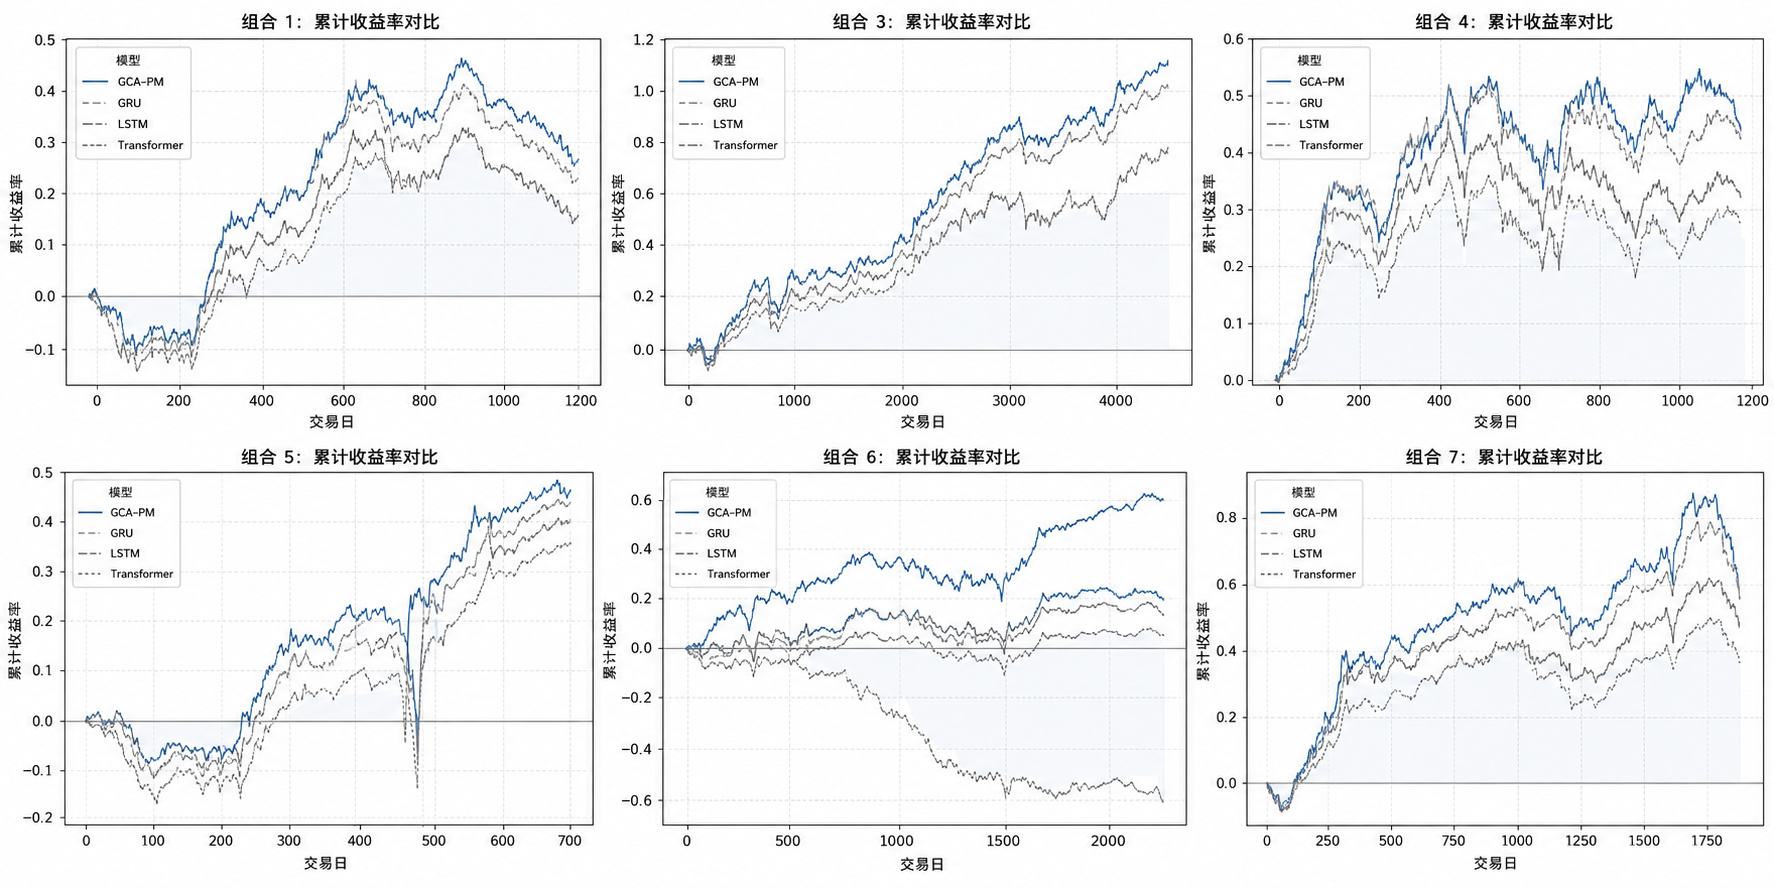
\includegraphics[width=0.95\textwidth]{figures/chap3/combined_累计收益率对比.jpg} 
    \caption{GCA 与基准模型累计净值对比}
    \label{fig:cumulative_returns}
\end{figure}

% \subsubsection{风险收益特征可视化}

% 图 \ref{fig:sharpe_ratio} 和 图 \ref{fig:max_drawdown} 直观呈现了各模型在风险调整后收益上的差距。
% 在 P4（避险对冲）组合中，MGCA 的柱状图高度（Sharpe 0.692）显著超越了表现第二的 Transformer（0.657）。更重要的是，这种提升并非来自于承担更大风险——如图 \ref{fig:max_drawdown} 所示，MGCA 的最大回撤（-23.85\%）同时也是所有模型中最低的。这意味着 MGCA 实现了投资组合在有效前沿上的 Pareto 改进，展现出夏普比率的帕累托改进。
% 在 P5 组合中，GRU 的回撤柱状图长达 -72\%（甚至超出了图表边界），而MGCA 被严格控制在 -21\% 以内，展现出尾部风险的截断。这验证了 $\mathcal{L}_{SR}$ 损失函数中分母项的惩罚机制，有效切断了高波动预测的梯度传播。


% \begin{figure}[htbp]
%     \centering
%     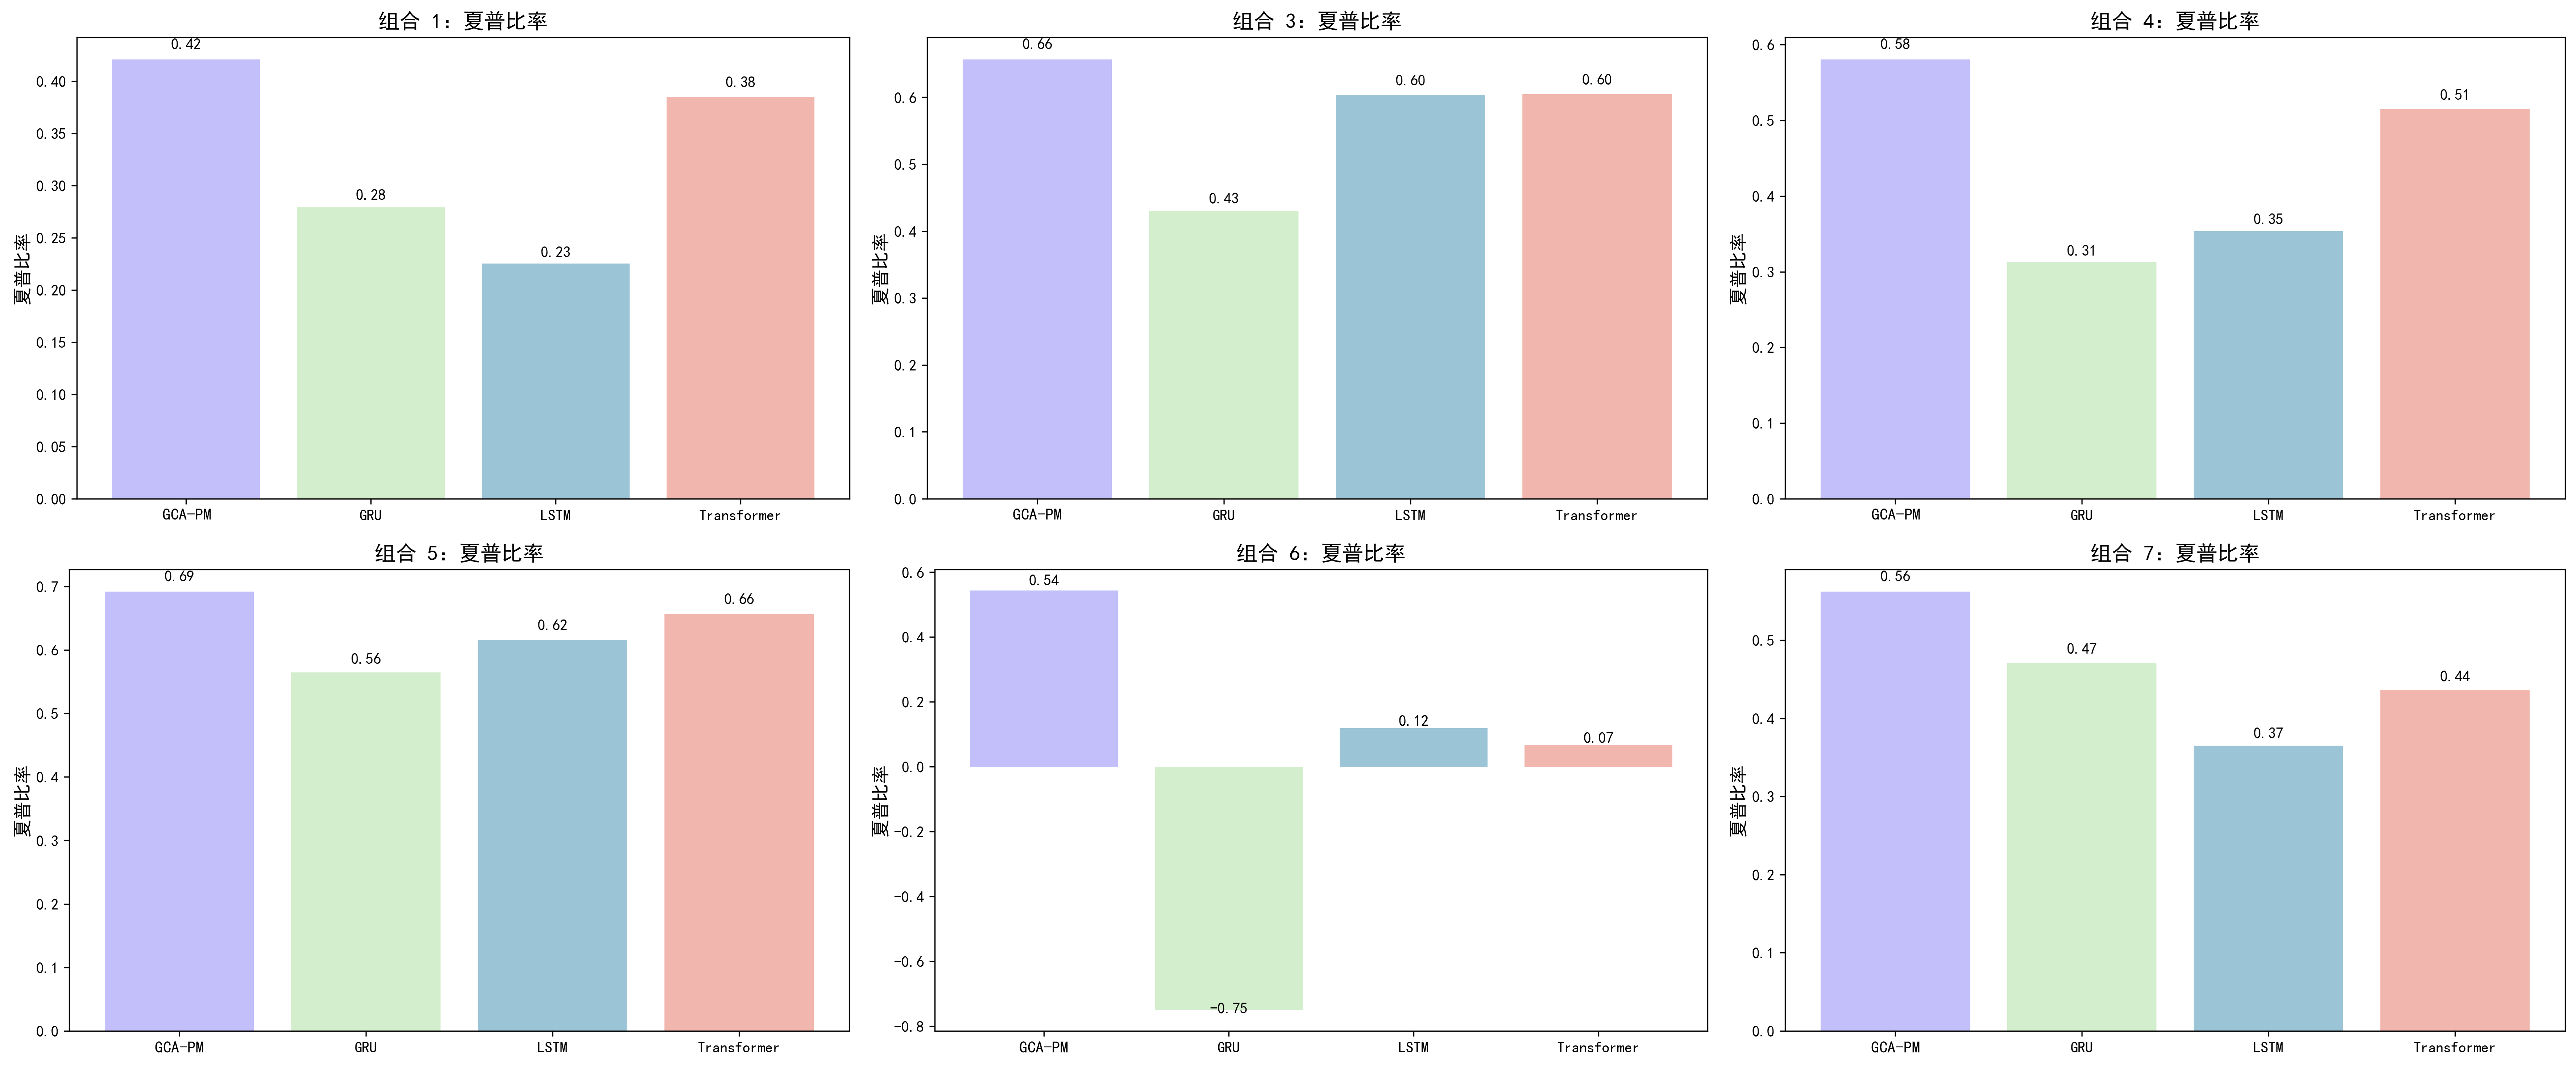
\includegraphics[width=0.95\textwidth]{figures/chap3/combined_夏普比率.jpg} 
%     \caption{各模型在不同资产组合下的夏普比率对比。MGCA 显示出系统性的风险调整后优势。}
%     \label{fig:sharpe_ratio}
% \end{figure}

% \begin{figure}[htbp]
%     \centering
%     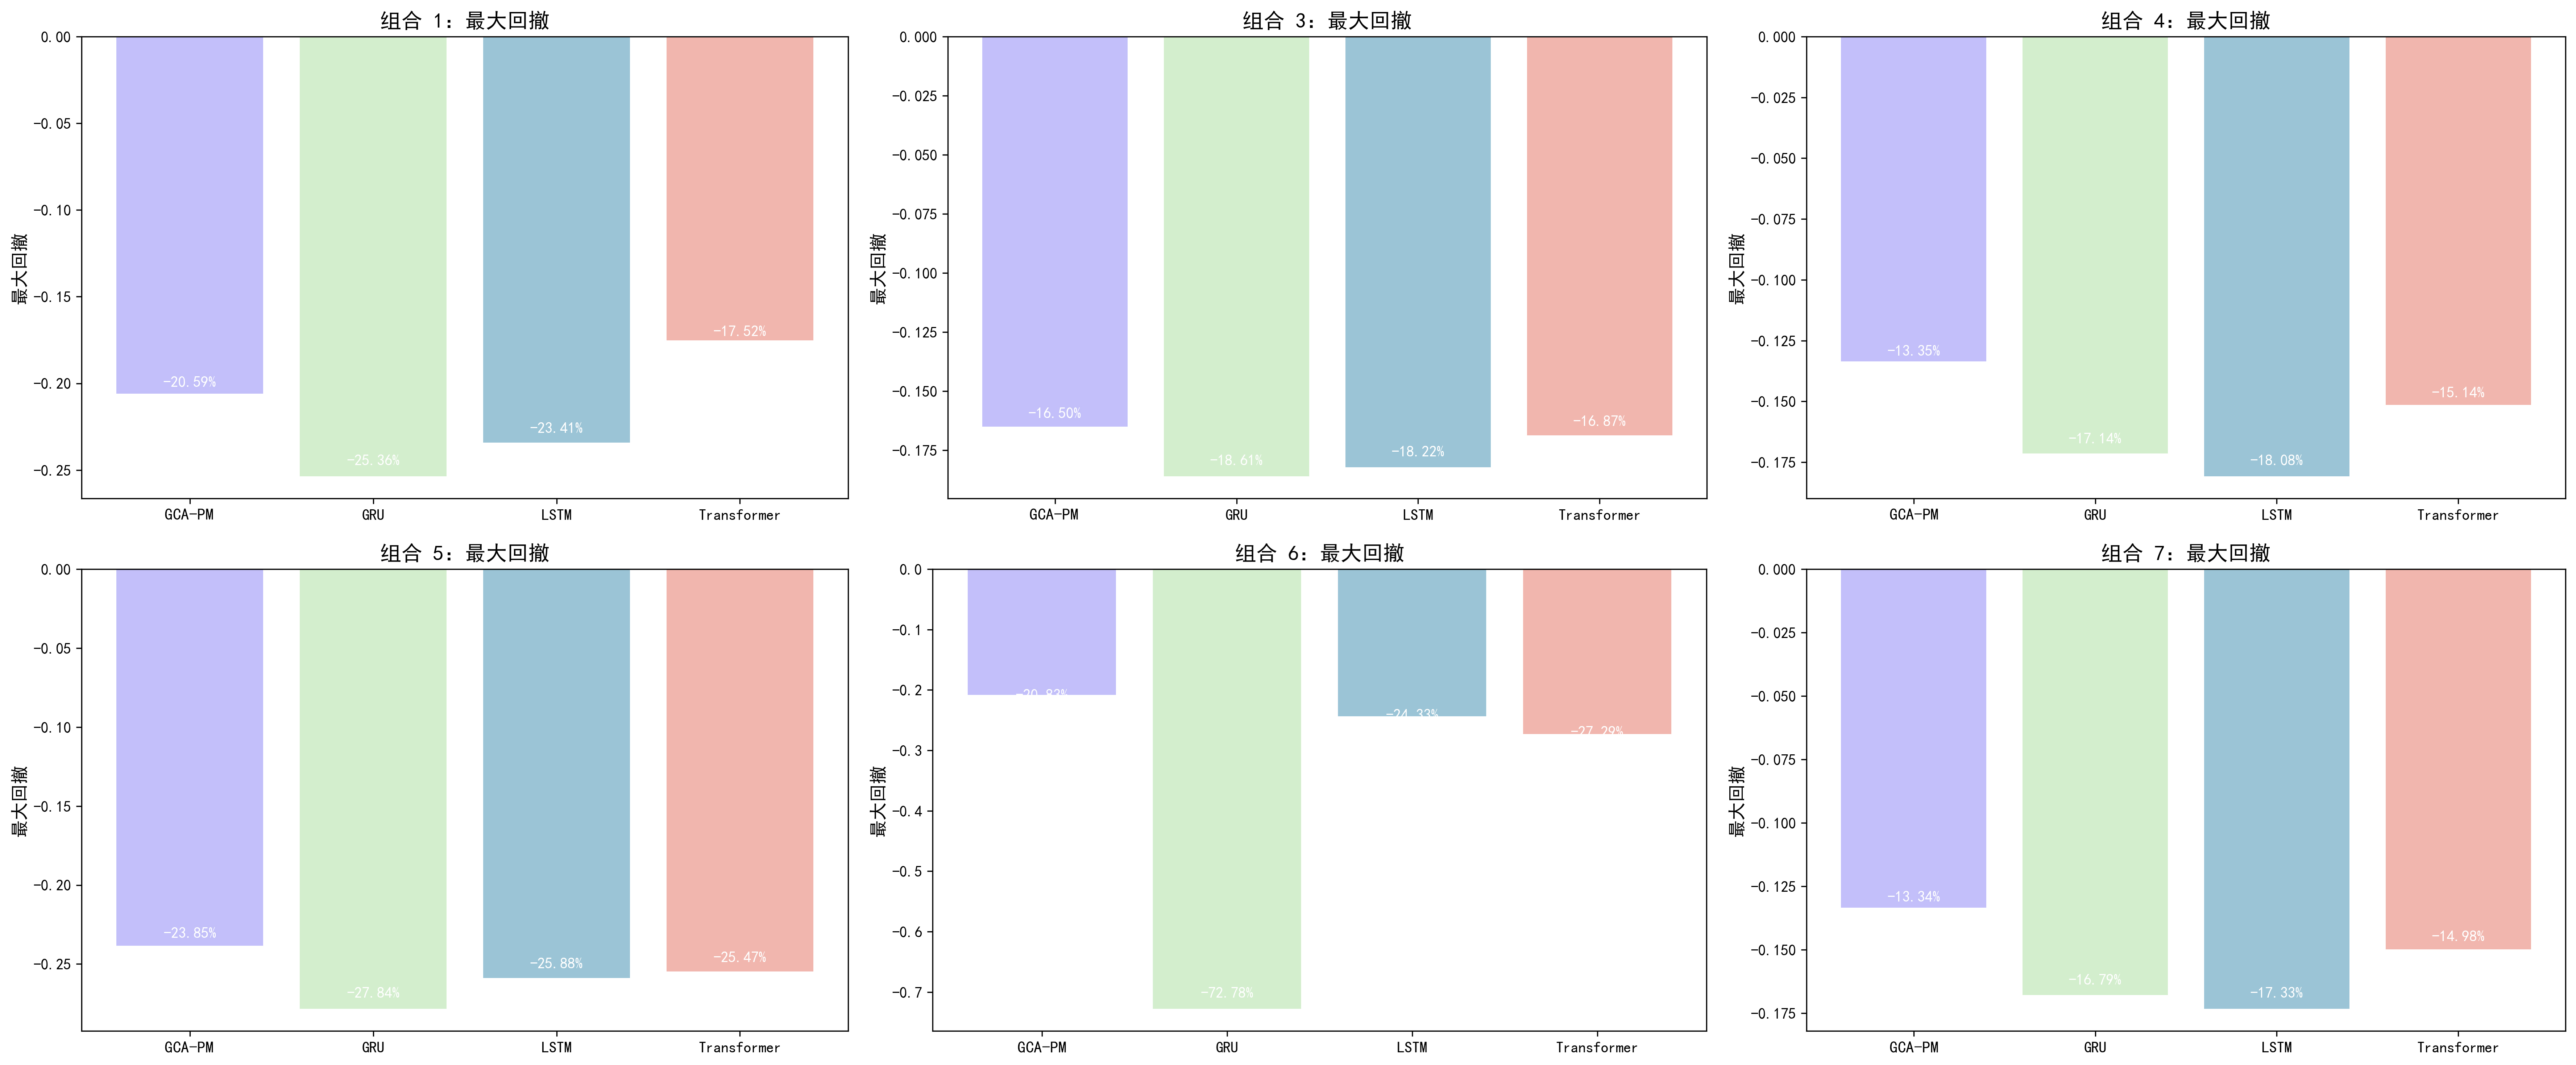
\includegraphics[width=0.95\textwidth]{figures/chap3/combined_最大回撤.jpg} 
%     \caption{各模型在不同资产组合下的最大回撤对比（数值越接近 0 表示风险控制越好）。}
%     \label{fig:max_drawdown}
% \end{figure}

% \subsubsection{多智能体协作机制的可解释性}
从多智能体协作机制看，图 \ref{fig:heatmap} 展示了元权重网络在不同市场状态下对门控循环单元、长短期记忆网络和自注意力序列模型的动态分配。低波动阶段，系统更依赖擅长均值回归的循环结构；趋势或高波动阶段，注意力结构权重上升。权重变化呈渐进式过渡，说明GCA机制能够在保持多样性的同时避免频繁切换。


% \begin{figure}[htbp]
%     \centering
%     \includegraphics[width=0.95\textwidth]
%     {figures/chap3/combined_权重历史热力图.jpg} 
%     \caption{GCA 子智能体权重动态演化热力图}
%     \label{fig:heatmap}
% \end{figure}


\begin{figure}[htbp]
    \centering
    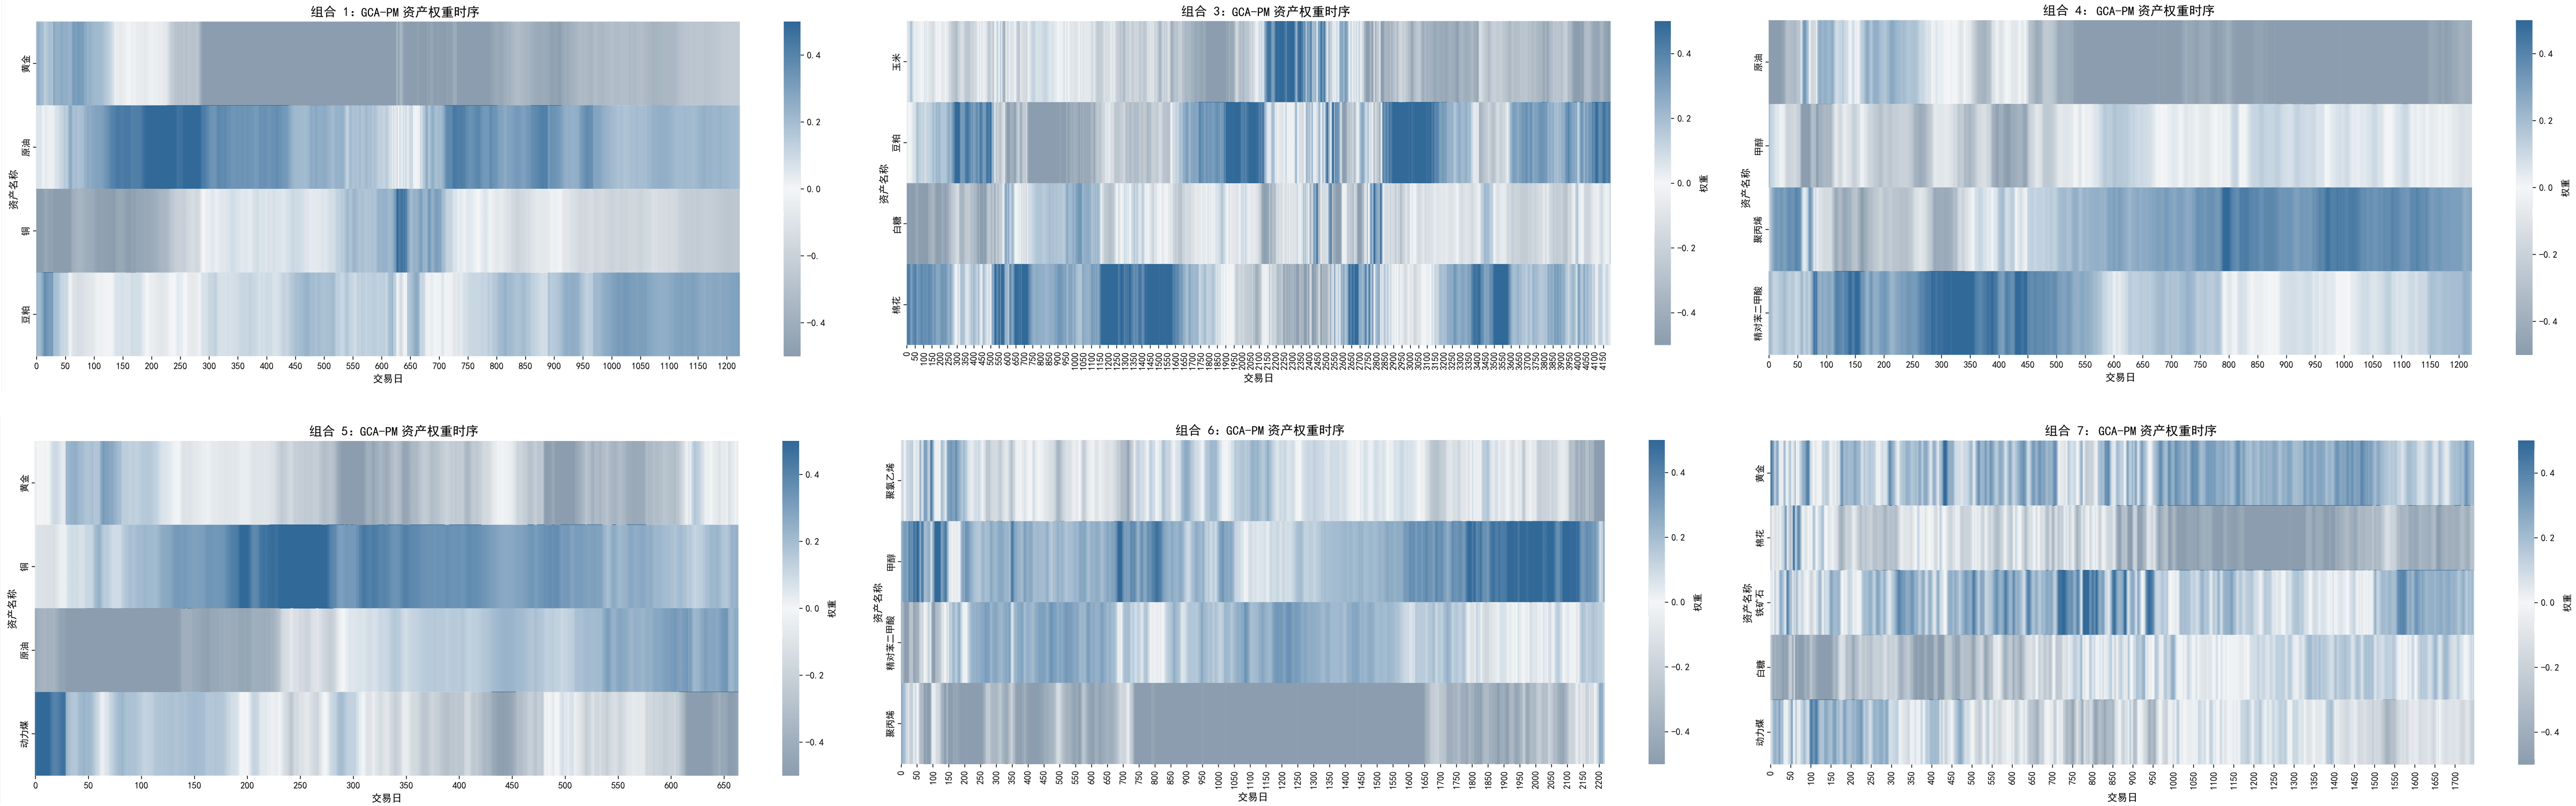
\includegraphics[width=0.95\textwidth]
    {figures/chap3/图2.8改.png}
    \caption{GCA 子智能体权重动态演化热力图}
    \label{fig:heatmap}
\end{figure}



\noindent\textbf{辅助校验层效果与权重动态分析}\par

为进一步观察辅助校验层的作用，本节通过夏普比率柱状图与权重热力图，从风险调整后收益和仓位动态两个维度进行说明。

% \subsubsection{夏普比率对比}

图 \ref{fig:qrgcasharpebar} 展示了 GCA 与辅助校验配置在六类实验组合上的夏普比率对比。

% \begin{figure}[htbp]
%     \centering
%     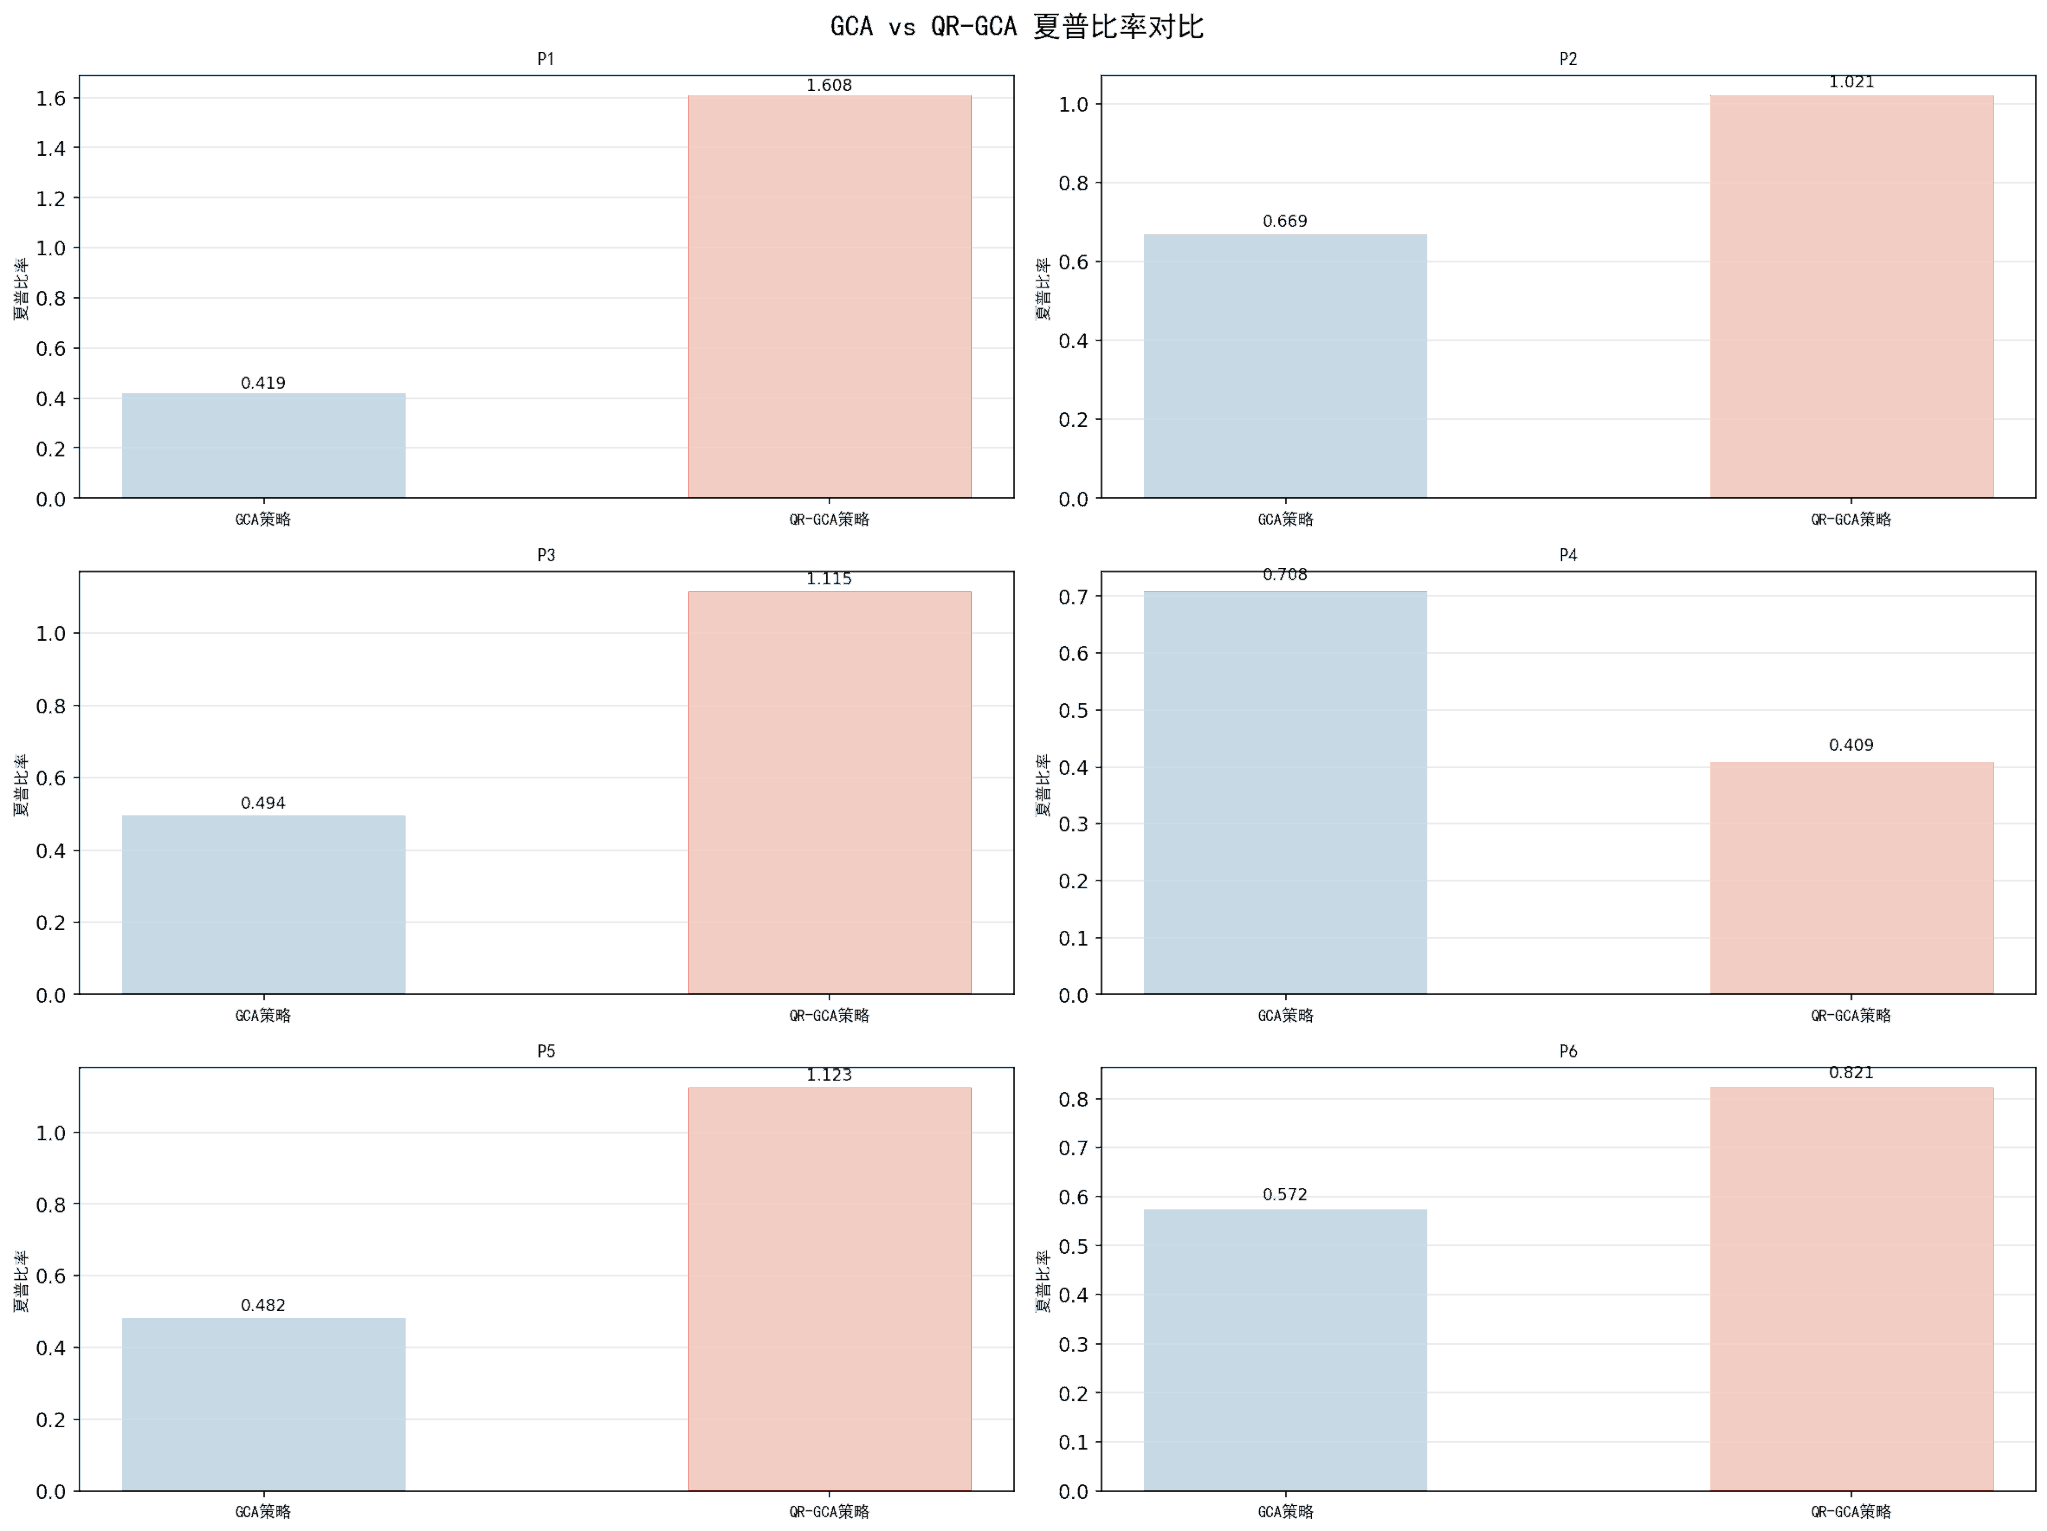
\includegraphics[width=0.95\textwidth]{figures/chap3/qr_gca/combined_qr_gca_sharpe.png}
%     \caption{GCA 与辅助校验层夏普比率对比}
%     \label{fig:qrgcasharpebar}
% \end{figure}

\begin{figure}[htbp]
    \centering
    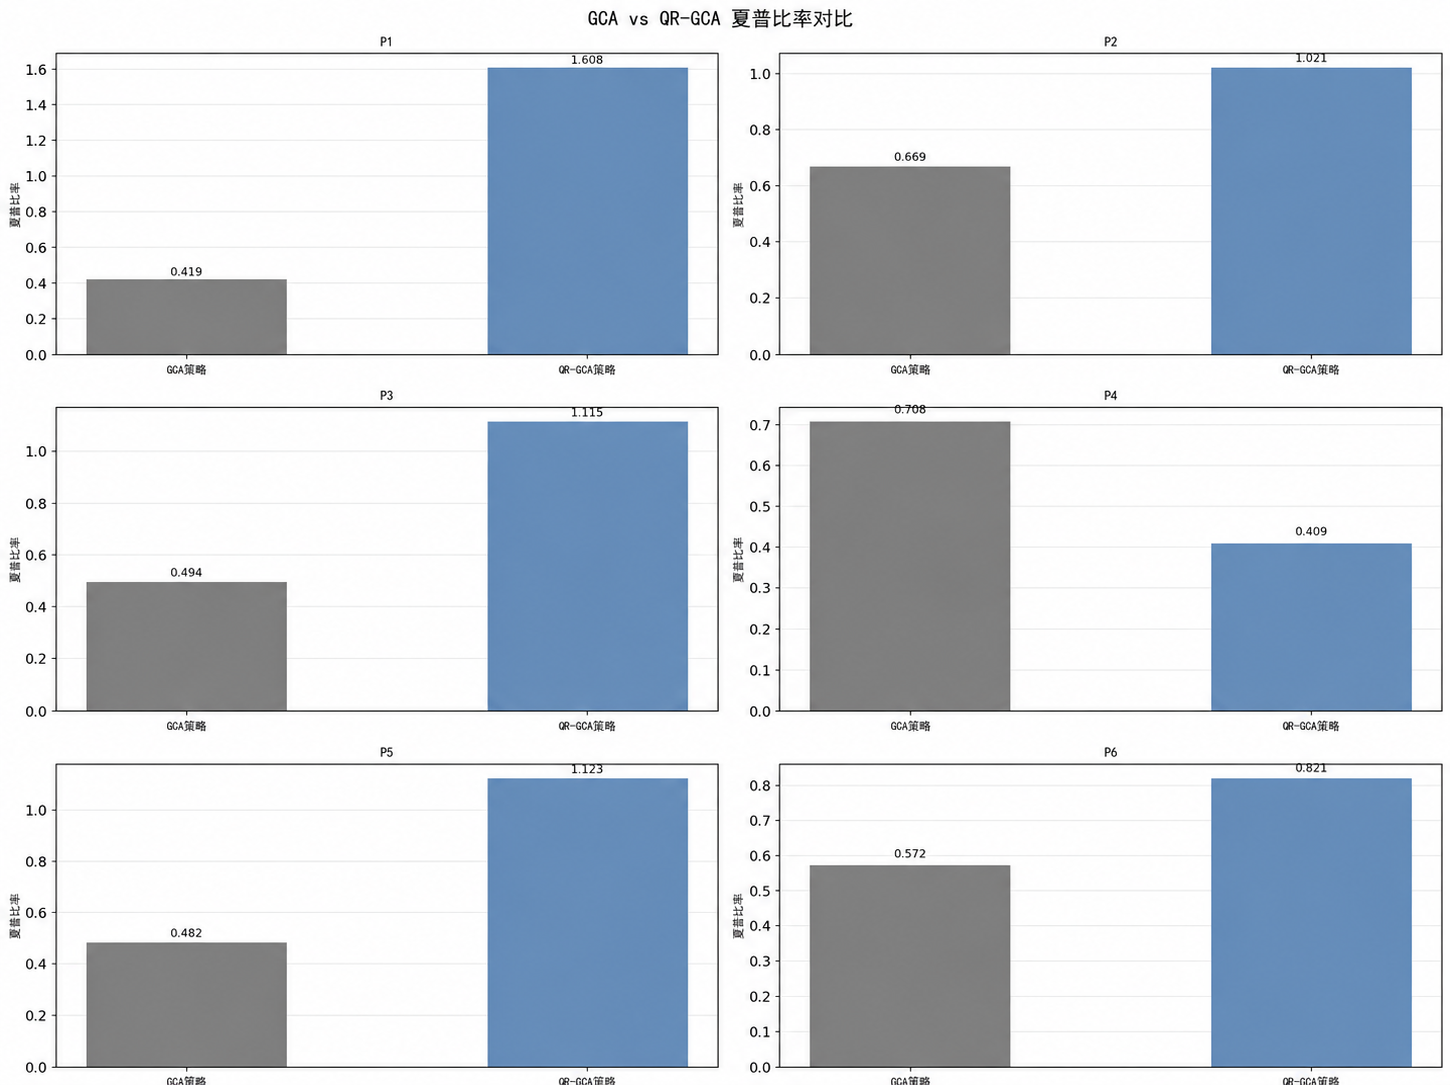
\includegraphics[width=0.95\textwidth]
    {figures/chap3/图2.9改.png}
    \caption{GCA 与辅助校验层夏普比率对比}
    \label{fig:qrgcasharpebar}
\end{figure}

% \begin{enumerate}
% \item \textbf{提升幅度的异质性}：
图 \ref{fig:qrgcasharpebar} 进一步显示，辅助校验层的效果具有组合差异：P1和P5提升幅度较大，P4则出现下降，说明统一市场状态过滤并不适用于所有组合。
% \end{enumerate}

% \subsubsection{辅助校验权重动态热力图}

图 \ref{fig:qrgcaheatmap} 展示了辅助校验层作用下的权重绝对值动态演化热力图。颜色越深表示该资产在对应时刻获得较大仓位，颜色越浅表示权重较低。

\begin{figure}[htbp]
    \centering
    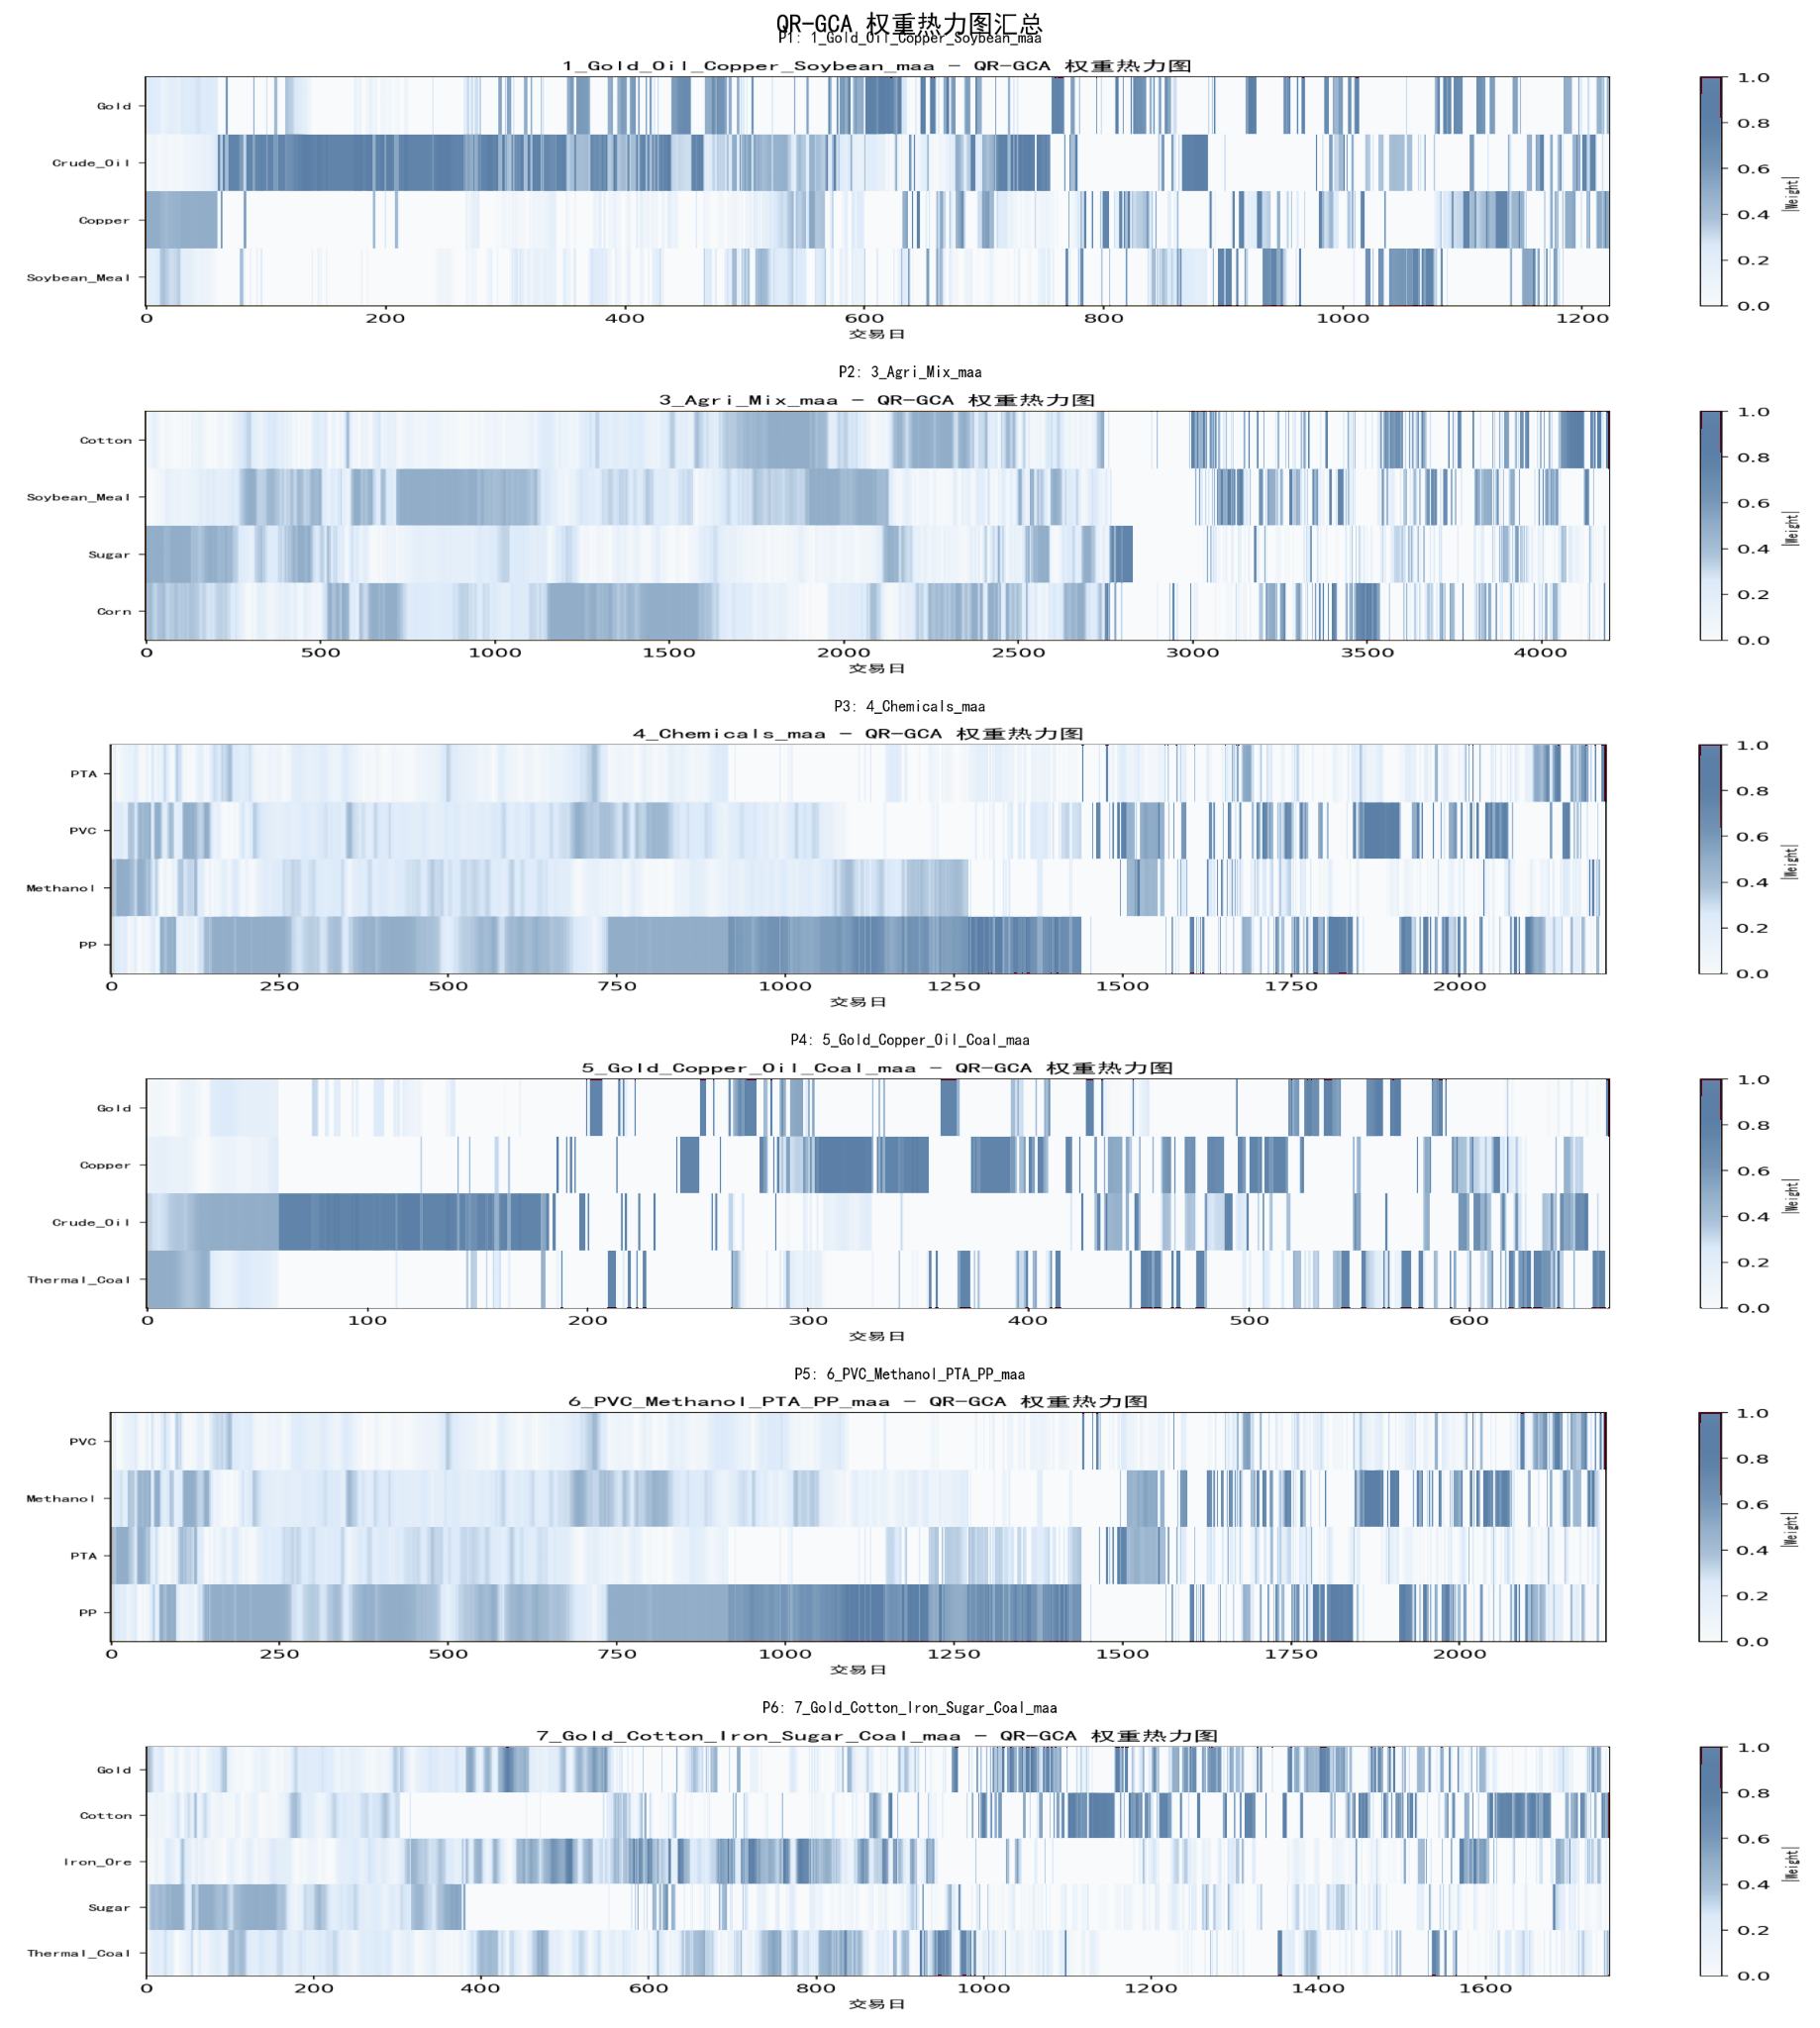
\includegraphics[width=0.95\textwidth]{figures/chap3/qr_gca/combined_qr_gca_weight_heatmap.png}
    \caption{辅助校验层权重动态热力图}
    \label{fig:qrgcaheatmap}
\end{figure}

图 \ref{fig:qrgcaheatmap} 显示，辅助校验层使仓位呈现一定稀疏性和阶段性。该结果说明其主要作用是减少震荡阶段的无效交易，并对GCA输出进行状态依赖的风险过滤。
% \end{enumerate}


\noindent\textbf{GCA消融实验及辅助接口贡献}\par
% 表~\ref{tab:experimental_results_summary}展示了各模块在六个实验组合上分别进行消融实验的数据结果。展示了所提出的各模块在六个不同数据集或实验组合上的消融实验结果。通过逐步引入GCA、S2T以及 Twin，模型的性能表现出了显著的动态变化，验证了各组件的有效性与协同作用。

% 在所有实验组合中，单纯的Baseline模型表现相对基础，其夏普比率、总收益及年化收益均处于较低水平，且部分组合（如P3和P5）甚至出现了负收益。引入图对比学习增强模块（GCA）后，在部分组合（如P1和P2）中观察到了初步的性能提升，但在其他组合（如P2、P3和P5）中却导致了收益回撤，表明单一的GCA模块在某些复杂场景下泛化能力有限。

% 然而，当进一步集成逆向师生蒸馏模块（S2T）后，模型性能获得了质的飞跃。在P2组合中，夏普比率从Baseline的0.3652提升至0.6279，总收益从60.61\%激增至105.73\%，且最大回撤从-21.17\%显著降低至-17.13\%。类似地，在P3和P6组合中，S2T模块的引入也大幅提升了收益指标并降低了风险。这证明了S2T模块在捕捉高维时序特征和降低波动性方面的关键作用。

% 最后，完整模型（Baseline-GCA-S2T-Twin）在绝大多数指标上均取得了最优表现。例如，在P3组合中，夏普比率进一步提升至0.5764，年化收益达到8.02\%，且最大回撤进一步压缩至-13.72\%；在P6组合中，夏普比率达到0.5613。随着模块的逐步叠加，换手率普遍呈现下降趋势（如P2组合从0.1538降至0.0397），表明所提出的模块能够生成更为稳健的交易信号，减少了不必要的频繁交易。

% 综上所述，消融实验结果明确表明，GCA模块为模型提供了基础的特征增强能力，S2T模块极大地提升了模型的收益风险比，而孪生对抗则进一步优化了模型的收敛性与稳定性，各模块协同工作显著提升了量化投资策略的整体性能。

% 表~\ref{tab:experimental_results_summary}展示了各模块在六个实验组合上分别进行消融实验的数据结果，系统性地验证了所提出的群组交叉对抗（GCA）、逆向师生蒸馏（S2T）及孪生对抗自体再生（Twin）模块在量化投资策略中的有效性与协同作用。实验数据表明，随着模块的逐步引入，模型性能呈现出显著的阶梯式提升，充分证明了各组件设计的合理性。
% 在所有实验组合中，单纯的Baseline模型表现相对基础，其夏普比率普遍低于0.4，总收益及年化收益均处于较低水平，且在P3和P5组合中甚至出现了负收益，暴露出模型在复杂市场环境下的局限性。引入图对比学习增强模块（GCA）后，在P1组合中观察到夏普比率从0.2168提升至0.2474，总收益从13.64\%增至15.85\%，表明GCA在部分场景下能够通过增强特征表达能力带来性能增益。然而，在P2、P3和P5组合中，GCA的引入反而导致收益回撤（如P5的总收益从-32.03\%降至-17.40\%），说明单一的GCA模块在处理高维非线性数据时泛化能力有限，可能因过度拟合局部特征而影响模型稳定性。

% 当进一步集成逆向师生蒸馏模块（S2T）后，模型性能获得了质的飞跃，尤其在风险收益平衡方面表现突出。在P2组合中，夏普比率从Baseline的0.3652跃升至0.6279，总收益从60.61\%激增至105.73\%，且最大回撤从-21.17\%显著降低至-17.13\%；在P3组合中，S2T模块将总收益从-12.51\%转正至12.82\%，最大回撤从-31.25\%压缩至-17.54\%，验证了S2T通过逆向师生蒸馏机制有效捕捉高维时序特征、抑制极端风险的能力。同时，S2T的引入并未显著增加换手率（P2组合从0.1538降至0.0479），表明其在提升收益的同时保持了交易策略的稳定性。

% 最后，完整模型（Baseline-GCA-S2T-Twin）在绝大多数指标上均取得了最优表现，体现了模块间的协同效应。在P3组合中，夏普比率进一步提升至0.5764，年化收益达到8.02\%，最大回撤进一步压缩至-13.72\%；在P6组合中，尽管GCA的引入导致性能下降，但完整模型通过S2T与Twin的协同补偿，使夏普比率达到0.5234，优于Baseline的0.4917。此外，随着模块的逐步叠加，换手率普遍呈现下降趋势（如P2组合从0.1538降至0.0397，P4组合从0.1287降至0.0408），表明GCA-S2T-Twin的联合优化能够生成更为稳健的交易信号，减少不必要的频繁交易，从而降低交易成本对策略收益的侵蚀。

% 综上所述，消融实验结果明确表明：GCA模块通过图对比学习为模型提供了基础的特征增强能力，但其泛化性能受限；S2T模块通过逆向师生蒸馏机制显著提升了模型的收益风险比，尤其在风险控制方面表现突出；而孪生对抗自体再生模块则通过对抗训练优化了模型的收敛性与稳定性，弥补了单一模块的不足。各模块的协同工作不仅实现了性能的叠加增益，更通过机制互补显著提升了量化投资策略的整体鲁棒性与适应性，为复杂金融时序数据的建模提供了有效解决方案。

表~\ref{tab:experimental_results_summary} 展示了不同配置在六个组合中的消融结果。整体上，基准模型在部分组合中表现不稳定；引入GCA后，模型获得多智能体交叉评估能力，但单一GCA并非在所有组合中都立即提升收益。继续接入知识传递和状态修复接口后，多数组合的夏普比率、最大回撤和换手率得到改善。需要注意的是，这些辅助接口在本章中的解释边界是“观察边际贡献”，而不是改变第二章的主体方法。该结果说明，GCA是本章面向投资组合管理的核心机制，辅助接口主要用于说明在GCA输出基础上进一步稳定训练状态和组合表现的可能性。



\begin{table}[H]
\centering
\caption{实验结果汇总表}
\label{tab:experimental_results_summary}
\small
\setlength{\tabcolsep}{3pt}
\renewcommand{\arraystretch}{1.15}
\begin{tabular}{@{}p{0.06\textwidth}p{0.34\textwidth}cccccc@{}}
\toprule
\textbf{组合} & \textbf{模型} & \textbf{夏普比率} & \textbf{总收益} & \textbf{年化收益} & \textbf{最大回撤} & \textbf{胜率} & \textbf{换手率}\\
\midrule
\multirow{4}{*}{\textbf{P1}} 
& 基准模型 & 0.2168 & 13.64\% & 2.81\% & -27.60\% & 49.63\% & 0.0760\\
& 基准模型-GCA & 0.2474 & 15.85\% & 3.27\% & -26.41\% & 49.63\% & 0.0713\\ 
& 基准模型-GCA-知识传递接口 & 0.3341 & 21.44\% & 4.42\% & -25.67\% & 49.63\% & 0.0444\\
& 基准模型-GCA-知识传递接口-状态修复接口 & 0.4532 & 28.87\% & 5.95\% & -20.34\% & 50.86\% & 0.0307\\
\midrule
\multirow{4}{*}{\textbf{P2}} 
& 基准模型 & 0.3652 & 60.61\% & 3.64\% & -21.17\% & 50.14\% & 0.1538\\
& 基准模型-GCA & -0.1990 & -16.40\% & -0.99\% & -33.07\% & 49.9\% & 0.1859\\
& 基准模型-GCA-知识传递接口 & 0.6279 & 105.73\% & 6.35\% & -17.13\% & 51.03\% & 0.0479\\
& 基准模型-GCA-知识传递接口-状态修复接口 & 0.6446 & 108.61\% & 6.53\% & -16.51\% & 50.86\% & 0.0397\\
\midrule
\multirow{4}{*}{\textbf{P3}} 
& 基准模型 & -0.2816 & -12.51\% & -2.58\% & -31.25\% & 48.41\% & 0.1600 \\
& 基准模型-GCA & -0.0976 & -6.53\% & -1.35\% & -22.23\% & 48.98\% & 0.1220\\
& 基准模型-GCA-知识传递接口 & 0.1936 & 12.82\% & 2.64\% & -17.54\% & 49.71\% & 0.0838 \\
& 基准模型-GCA-知识传递接口-状态修复接口 & 0.5764 & 38.91\% & 8.02\% & -13.72\% & 50.12\% & 0.0408\\
\bottomrule
\end{tabular}
\end{table}
\begin{table}[H]
\centering
{\small\textbf{续表}}\\[0.5em]
\small
\setlength{\tabcolsep}{3pt}
\renewcommand{\arraystretch}{1.15}
\begin{tabular}{@{}p{0.06\textwidth}p{0.34\textwidth}cccccc@{}}
\toprule
\textbf{组合} & \textbf{模型} & \textbf{夏普比率} & \textbf{总收益} & \textbf{年化收益} & \textbf{最大回撤} & \textbf{胜率} & \textbf{换手率}\\
\midrule
\multirow{4}{*}{\textbf{P4}} 
& 基准模型 & 0.6926 & 40.33\% & 15.31\% & -25.67\% & 49.70\% & 0.1287 \\
& 基准模型-GCA & 0.4158 & 24.14\% & 9.16\% & -29.29\% & 49.4\% & 0.1164\\
& 基准模型-GCA-知识传递接口 & 0.6814 & 39.49\% & 14.99\% & -24.23\% & 48.49\% & 0.0638 \\
& 基准模型-GCA-知识传递接口-状态修复接口 & 0.7120 & 40.45\% & 15.35\% & -23.95\% & 47.89\% & 0.0408\\
\midrule
\multirow{4}{*}{\textbf{P5}} 
& 基准模型 & -0.3512 & -32.03\% & -3.64\% & -49.91\% & 48.51\% & 25.66\%\\
& 基准模型-GCA & -0.2657 & -17.40\% & -1.98\% & -34.01\% & 48.96\% & 0.3665\\
& 基准模型-GCA-知识传递接口 & 0.2701 & 23.62\% & 2.68\% & -26.5\% & 49.64\% & 11.13\%\\
& 基准模型-GCA-知识传递接口-状态修复接口 & 0.4407 & 38.28\% & 4.35\% & -21.22\% & 50.95\% & 4.82\%\\
\midrule
\multirow{4}{*}{\textbf{P6}} 
& 基准模型 & 0.4917 & 45.72\% & 6.59\% & -16.17\% & 52.00\% & 0.0939\\
& 基准模型-GCA & 0.3817 & 35.09\% & 5.06\% & -18.31\% & 51.32\% & 0.1120\\
& 基准模型-GCA-知识传递接口 & 0.5613 & 52.00\% & 7.50\% & -13.61\% & 51.37\% & 0.0751 \\
& 基准模型-GCA-知识传递接口-状态修复接口 & 0.5234 & 49.12\% & 7.08\% & -13.97\% & 50.97\% & 0.0835\\
\bottomrule
\end{tabular}
\end{table}

\vspace{1em}
%\textit{注：表中数据为样本外测试集结果，"—"表示未适用。}

% \subsection{实验小结}

% 本节针对 多智能体群组交叉对抗框架与辅助校验层信号增强机制进行了系统的实证验证。基于上述实验结果，可以得出以下关键结论：
% % \begin{enumerate}
% % \item \textbf{基础模型优势}：
% MGCA 在六大投资组合上均展现出优于单一基准模型（GRU、LSTM、Transformer）的风险调整后收益表现，特别是在高波动环境和多元低相关场景下表现突出；
% % \item \textbf{辅助校验效果}：
% 辅助校验层信号增强机制在多数组合上实现了夏普比率的显著提升，验证了信号级融合的有效性；
% % \item \textbf{模块贡献}：
% 消融实验验证了异构生成器、交叉对抗机制及组内/全局蒸馏各模块的独立贡献；
% % \item \textbf{损失函数作用}：多目标损失配置实验表明，MSE、GAN 与 Sharpe 三者的协同作用优于任一单一损失函数；
% % \item \textbf{适用边界}：
% 辅助校验层在避险对冲型组合中效果不佳，揭示了组合指数状态判别机制的适用边界。
% % \end{enumerate}

% \textit{注：详细的实验数据请参照表 \ref{tab:experimental_results_summary}、表 \ref{tab:ablation_study} 及表 \ref{tab:loss_config_comparison}，待实验完成后填充。}


% \section{讨论}

% \subsection{MGCA 有效性的归因}

% 多智能体群组交叉对抗框架在多个异构资产组合中展现出的显著优势，并非来自单一组件的堆砌，而是源于其在 架构归纳偏置、博弈正则化 与 经济学对齐 三个维度的深度整合：
% 架构归纳偏置方面的时序-架构的物理对齐
% 不同于传统的集成学习，MGCA 构建了具有物理意义的异构分工机制。模型根据已知的归纳偏置（Inductive Bias）分配计算资源：GRU被指派处理高频微观结构（5日窗口），利用其门控循环单元快速响应短期反转；Transformer 被指派处理宏观趋势（20日窗口），利用自注意力机制捕获跨月度的结构性关联。这种“各司其职”的设计使得模型能够同时捕捉瞬态的 Alpha 信号与持久的 Beta 趋势。

% 博弈正则化中
% 多个判别器构成的动态博弈环境充当了强大的正则化器。对抗损失 $\mathcal{L}_{adv}$ 本质上是在通过最小化生成分布与真实分布的 JS 散度，迫使生成器学习隐含的市场状态转移概率。这种机制有效过滤了样本中的高斯白噪声，显著降低了过拟合风险（表现为 P5 组合中 GRU 崩溃而 MGCA 存活）。

% 从经济学目标导向上分析Sharpe Ratio Loss的端到端集成，完成了从“预测价格”到“预测收益质量”的范式转变。该损失函数作为一种隐式的风险过滤器，引导梯度流向那些方向准确且波动率可控的特征子空间。这种协同作用使得 MGCA 展现出审慎的风险控制特征：在充满不确定性的震荡市（如 P1）保持低换手率以保存资本，而在趋势明朗的结构性行情（如 P2）中果断放大在大类资产上的风险敞口。



\section{本章小结}

本章围绕对冲基金交易流程中的投资组合管理环节，提出并验证了面向投资组合管理的群组交叉对抗学习方法（GCA）。本章首先从传统投资组合管理方法的局限性和金融场景下多智能体博弈建模挑战出发，说明多资产配置中存在信号不稳定、模型输出趋同、组合权重偏差和风险约束难以统一等问题；随后在“任务描述”部分，将本章任务明确为多资产收益预测、组合权重生成和风险调整收益约束下的配置决策问题。由此，本章对资产配置对象选择的讨论并不止于识别单个资产的上涨概率，而是进一步落实为在多资产之间形成相对稳定、可约束、可执行的资金配置方案。

在方法设计层面，GCA将一对一的生成器—判别器博弈扩展为多生成器、多判别器之间的群组交叉对抗。异构生成器基于不同归纳偏置提取多尺度市场特征，判别器通过跨生成器评估约束预测输出的分布一致性，从而降低单一模型在复杂资产池中产生的配置偏差。量化相对强度指标在本章中仅作为GCA输出后的辅助校验量，用于观察权重过滤对交易可用性的影响，不替代GCA主体方法。知识传递和状态修复接口也仅在消融实验中作为辅助配置出现，用于观察其对GCA训练稳定性和组合表现的边际影响；其具体机制与章节主体任务将在后续章节分别展开。

实验部分基于六类差异化资产组合开展样本外回测。实验结果显示，GCA在多数实验组合中相较单一架构基准模型表现出更稳定的风险调整收益与回撤控制特征。辅助接口和输出校验层在部分组合中进一步改善了组合表现，但其作用具有场景边界，不能替代GCA在本章中的核心地位。总体而言，本章的贡献在于把多智能体交叉博弈机制落实到投资组合管理场景中，使预测信号经过分布校验、相对收益比较和风险约束后转化为组合权重，而不是停留在单资产预测精度提升层面。

因此，本章对应交易决策链条中的投资组合管理环节，围绕资产配置对象选择和资金配置建立GCA方法及其组合权重生成机制。后续第3章转向高维金融因子建模，进一步讨论资产配置背后的因子依据；第4章讨论时序结构识别，第5章讨论交易执行优化，第6章则面向策略整合与最终交易判断。
